\chapter{Frozen Showers}\label{chap:FS}
\minitoc


As it was mentioned in Chap.~\ref{chap:MC}, fast simulation techniques are an essential part of the Monte-Carlo production in the \atlas experiment. The typical time needed for simulating a $t\bar{t}$ event is around 1 minute, and most it is spent on the simulation of particle interaction in the calorimeters. This motivates the development of fast calorimetry techniques, allowing to describe calorimeter response.

In this chapter a Frozen Showers method for the forward calorimeter simulation is described. The first section gives a small introduction to the method. In the next section properties of the electron shower in the FCAL are showed. In the Sec.~\ref{sec:FSProdUse} the use of method is explained. The Sec.~\ref{sec:MLBinning} introduces a new method of finding the bin size for a libraries. Finally, in the last section, the validation of Frozen Showers is showed.

\section{Introduction}
Frozen showers is currently the main fast calorimeter simulation approach used at \atlas experiment\cite{FS}.  This method uses pre-simulated "frozen" showers. This allows to reduce the time spent on a simulation of a large amount of low energy sub showers. This method gives a 25\% speedup in simulation. It is required to have in advance generated libraries for each detector and particle used in this method. 

For each shower in the library its lateral and transverse size and a list of the all energy deposition inside the sensitive material (hits) with information about their energy, position and time are stored. During simulation, if the energy of a secondary electron falls below the cut-off energy it is replaced by a shower from a library, as shown in Fig.~\ref{fig:MC_FS_method}. Main parameters used in \atlas simulation are summarized in a Tab.~\ref{tab:MC_FS_params}, where FCAL1 and FCAL2 are the first two froward calorimeters (see Sec. \ref{sec:forwardCalo}) and $E_{\gamma}<10$, $E_{e}<1000$, $T_n<100$ are the maximum energies of photons, electrons and neutrons used in the method. 

Since currently the Frozen Showers method is used only for FCAL, this chapter will fully concentrate on optimisation of Frozen Showers in forward calorimeter.

\begin{figure}[!tbp]
\center{
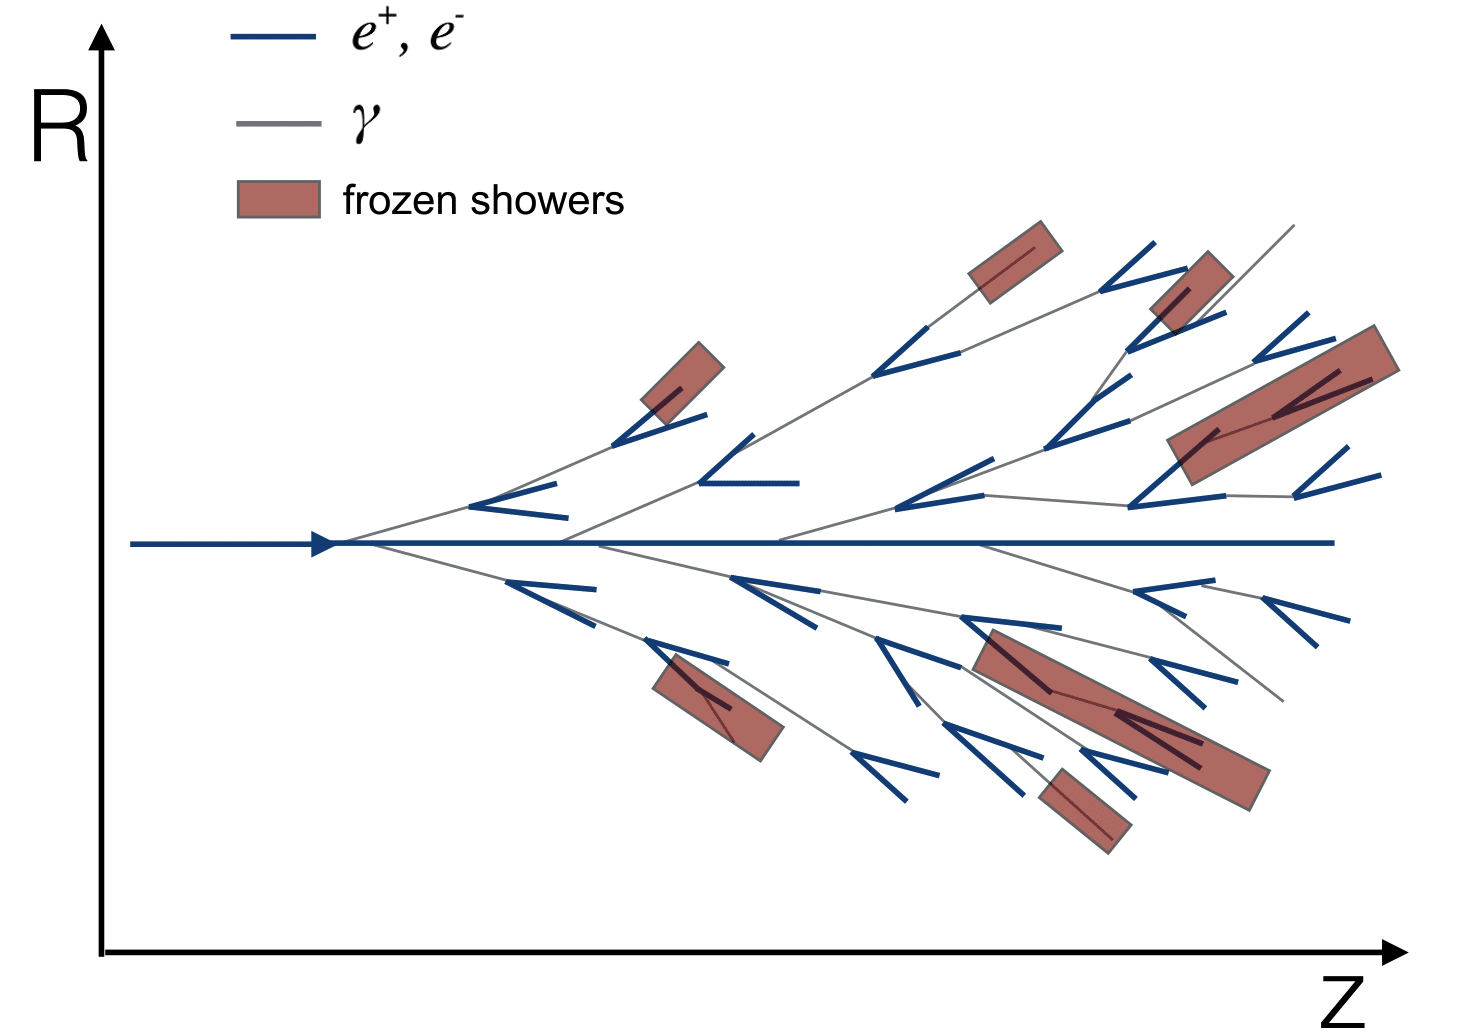
\includegraphics[width=0.9\textwidth]{MC/FSMethod2.png}
\caption{Diagram showing the shower substitution of the low-energy electron, during the high-energy particle simulation. Some of the showers from a particles, substituted by frozen showers method marked by a red squares}
\label{fig:MC_FS_method}
}
\end{figure}

\begin{table}[!tbp]
\caption{Main parameters used for the frozen shower libraries}
\label{tab:MC_FS_params}
\centering
\begin{tabular}{l|r}
\hline
\hline
\multicolumn{2}{c}{The general frozen showers parameters} \\
\hline
Detectors used            & FCAL1, FCAL2\\
Type of the particle      & photons, electrons, neutrons \\
Energy cut-off            &  $E_{\gamma}<10$~MeV,  $E_{e}<1000$~MeV,  $E_n<100$~MeV \\
\hline
\end{tabular}
\end{table}

\section{Properties of electron showers in FCAL}\label{sec:FSproblem}




%\begin{figure}[!b]
%\center{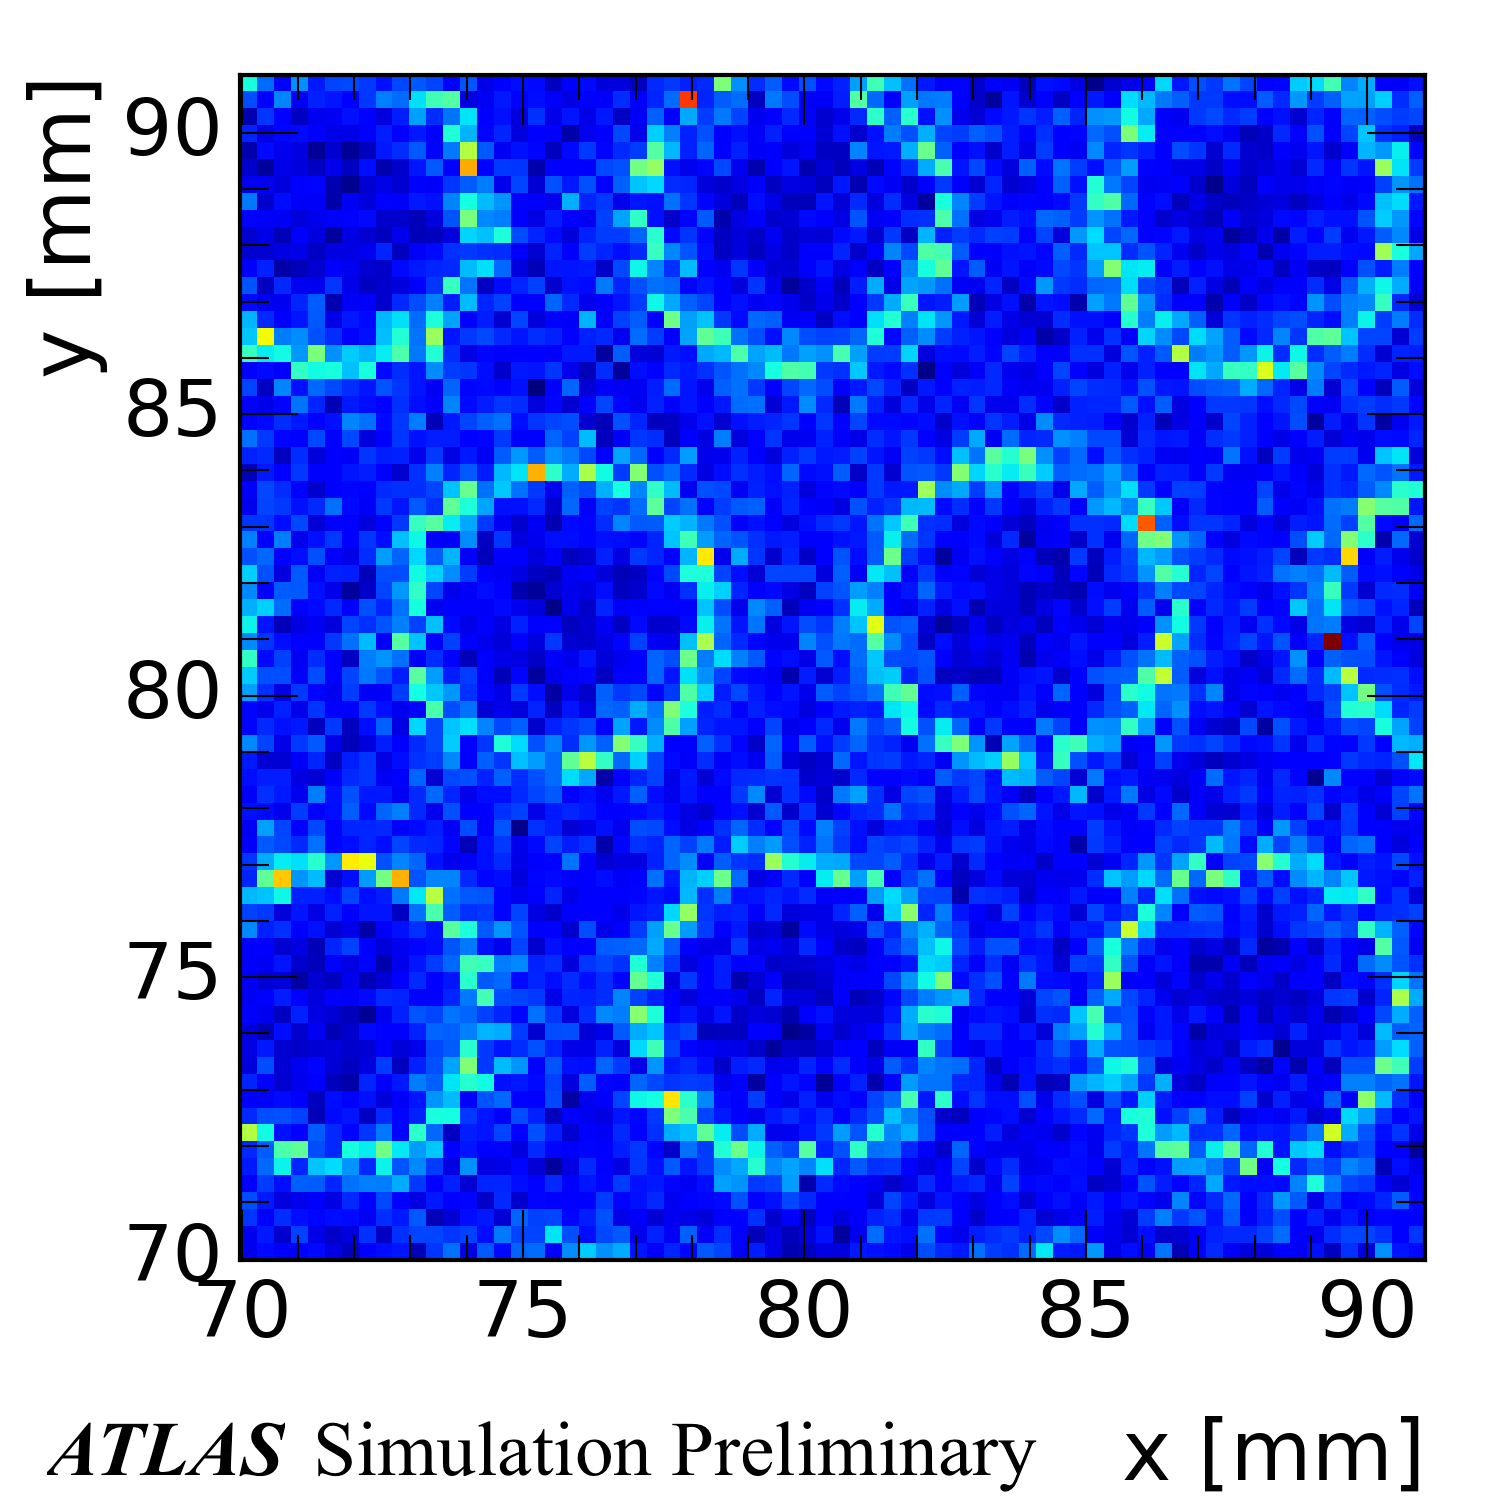
\includegraphics[width=0.5\linewidth]{MC/xySumE.png} }
%\caption{Shower energy response histogram in the x vs y plane for electrons, generated with uniformly distributed x and y and energy less than 1 GeV. Light circles are corresponding to a showers, started inside a LAr gaps with on average higher energy response, while the dark parts are corresponding to dead material respectively with smaller sum of the "hits" energy. }
%\label{fig:FSFluctuations}
%\end{figure}

\begin{figure}[!tbp]
\begin{minipage}[h]{0.49\linewidth}
\center{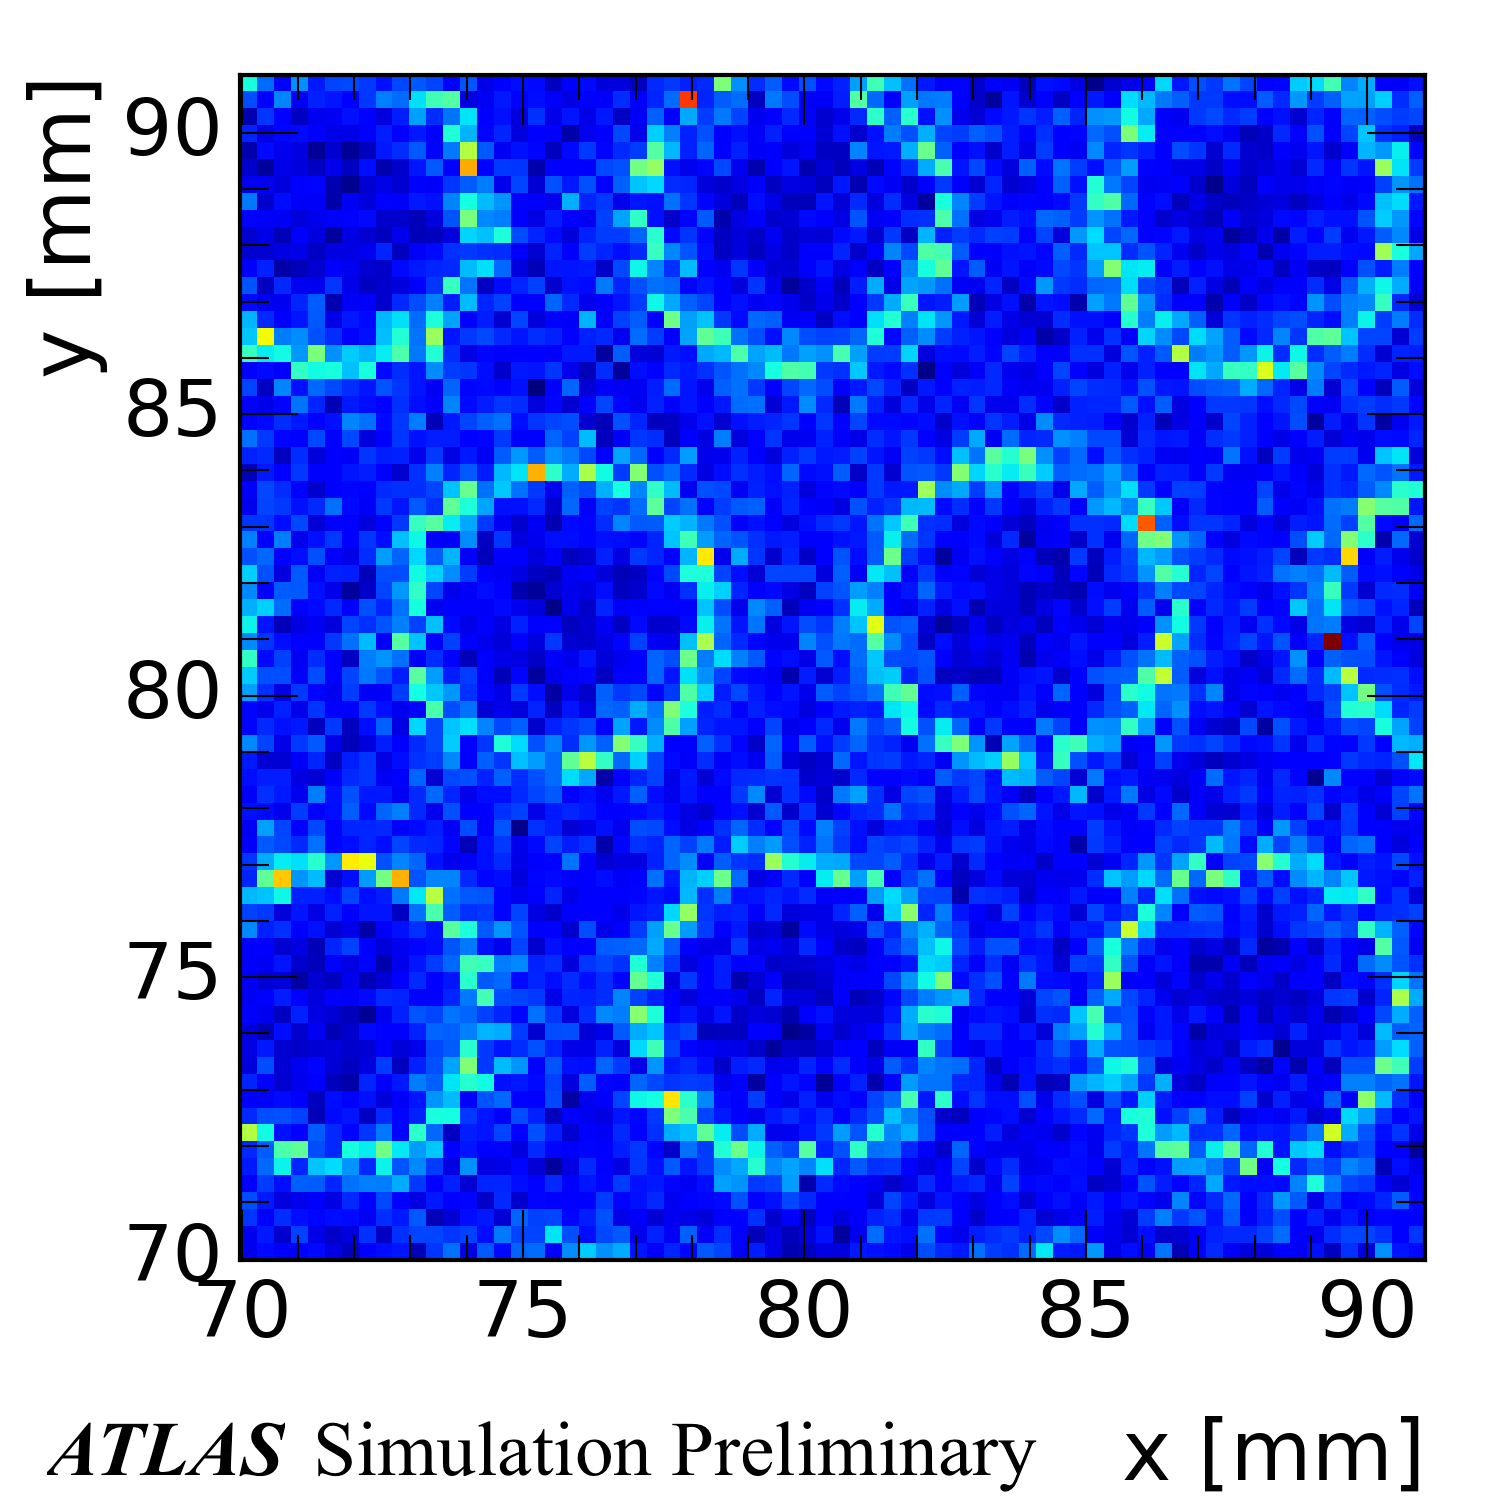
\includegraphics[width=0.9\linewidth]{MC/xySumE.png} \\ a)}
\end{minipage}
\hfill
\begin{minipage}[h]{0.49\linewidth}
\center{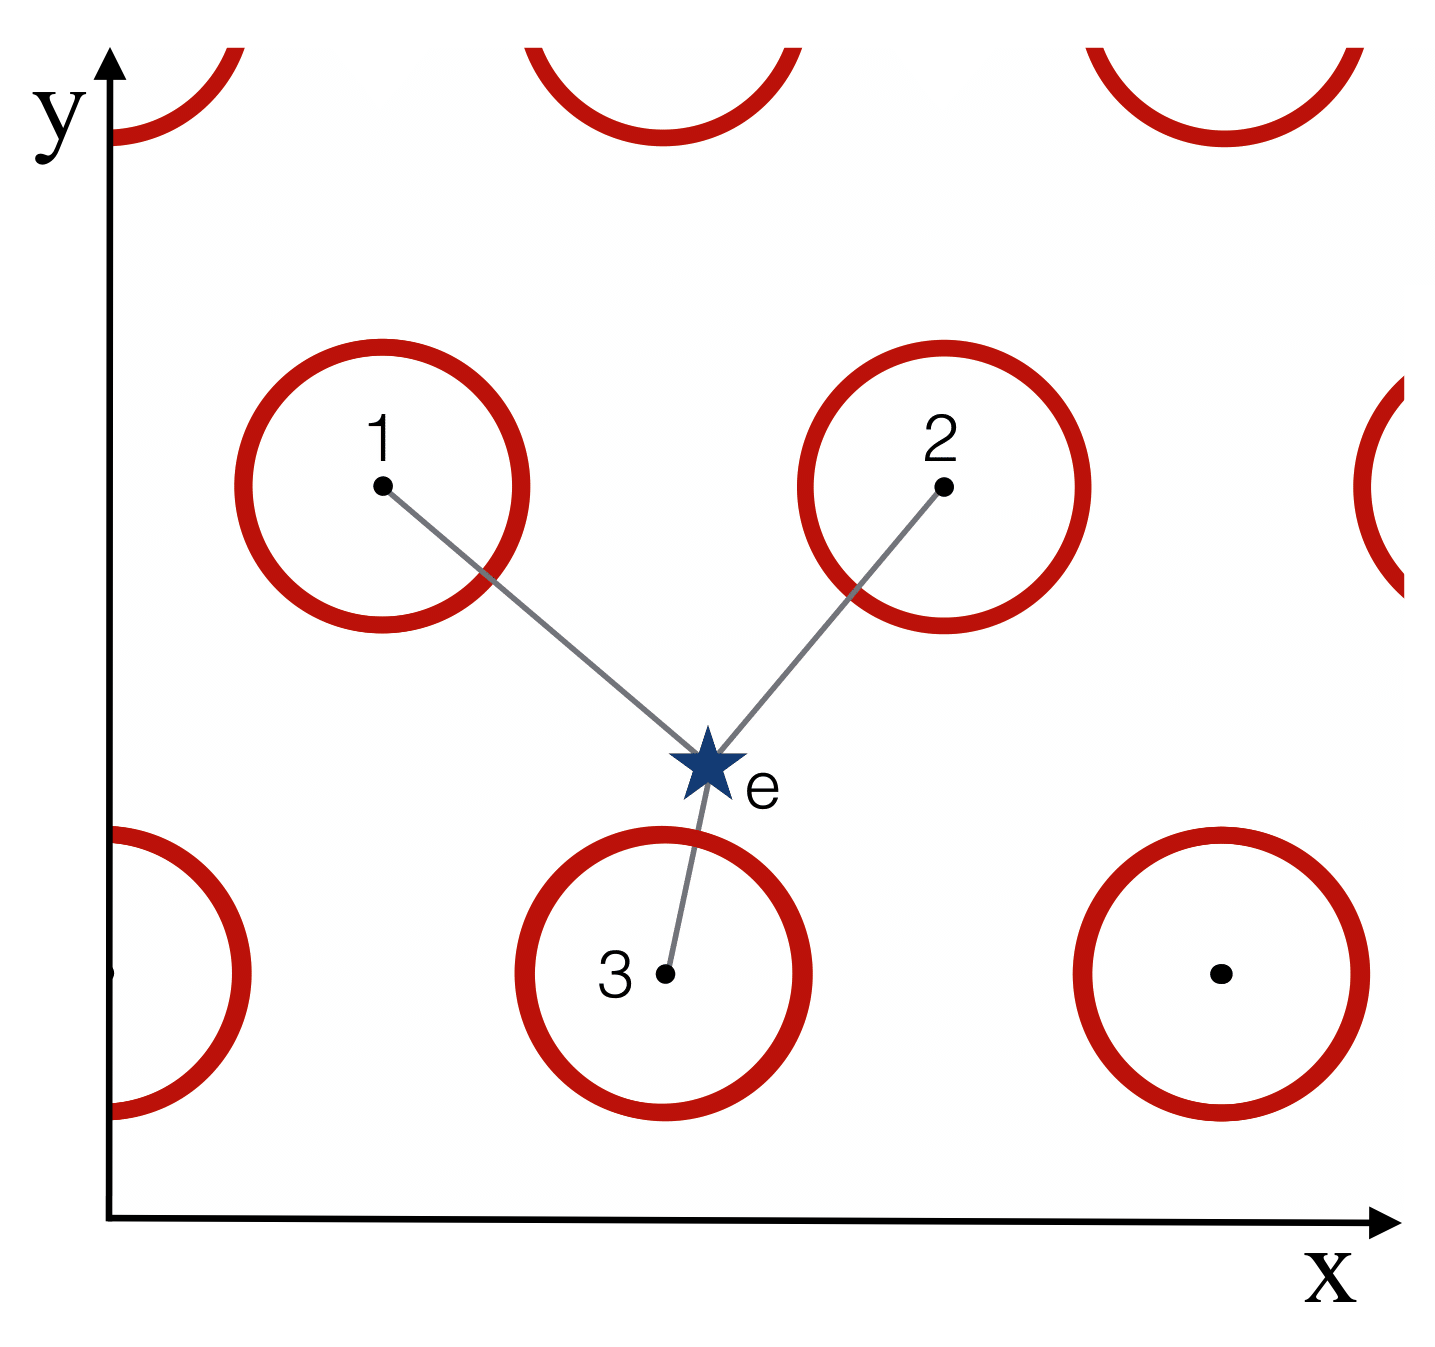
\includegraphics[width=0.9\linewidth]{MC/DistanceCalculation.png} \\b)}
\end{minipage}
\caption{ a) Shower energy response histogram in the transverse (x vs y) plane for electrons, generated with uniformly distributed x and y and total energy less than 1 GeV. Light circles correspond to showers, starting inside the LAr gaps with on average higher energy response, while the dark parts correspond to dead material with smaller sum of the "hits" energy respectively.
b) Distance to the closest rod center scheme $d_{rod} = min( d(1,e), d(2, e), d(3, e))$, where 1,2,3 are the positions of the rod centers and e is the position of initial electron. The rod centers and liquid argon gaps are shown by black dots and red circles respectively.}
%\caption{Distribution a) electron energies and b) mean number of hits in a shower vs energy of electron for electrons with energy less than 1 GeV coming from initial electron with energy 1 TeV. }
\label{fig:FSFluctuations}
\end{figure}


\begin{figure}[!tbp]
\begin{minipage}[h]{0.49\linewidth}
\center{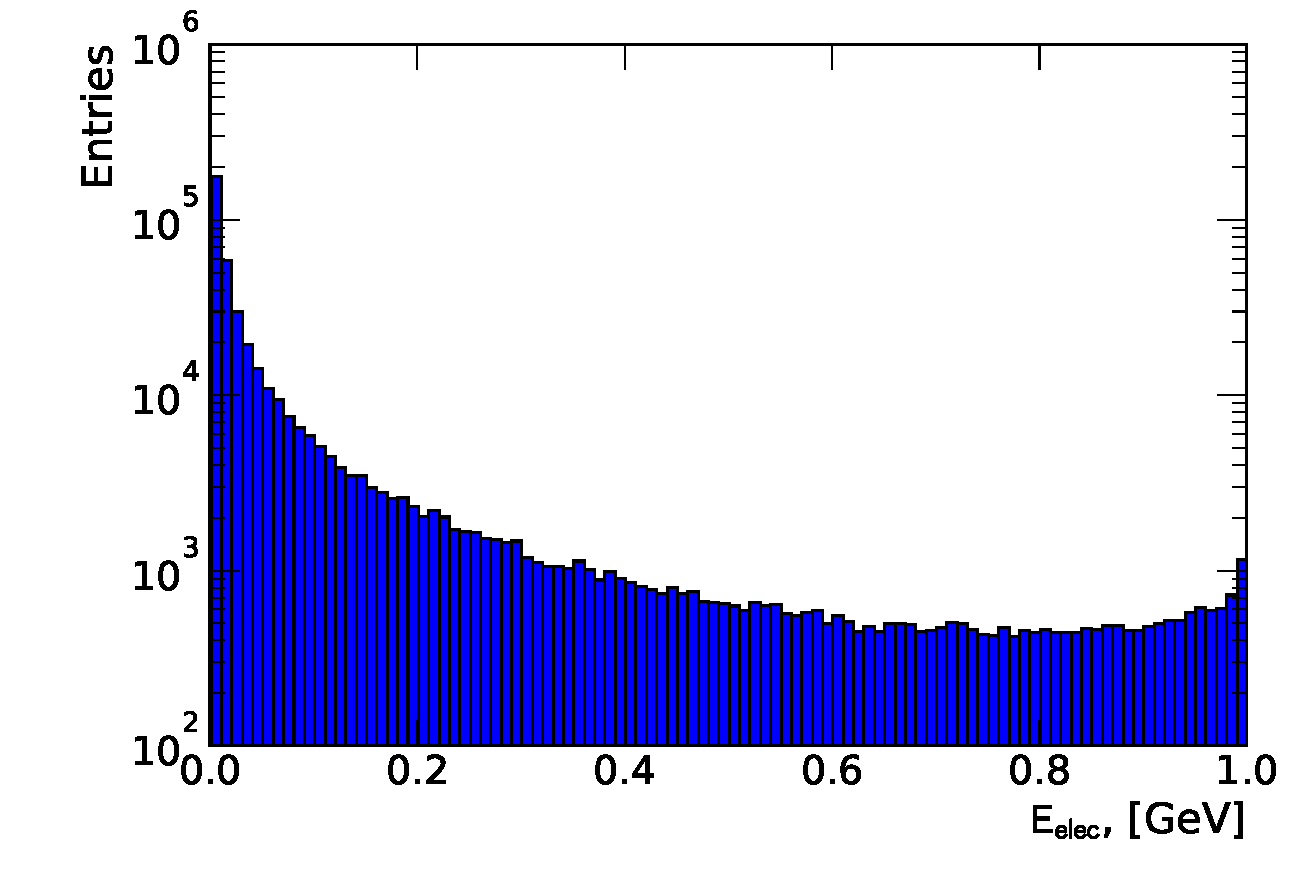
\includegraphics[width=1.0\linewidth]{MC/FSEnergy.pdf}  \\ a)}
\end{minipage}
\hfill
\begin{minipage}[h]{0.49\linewidth}
\center{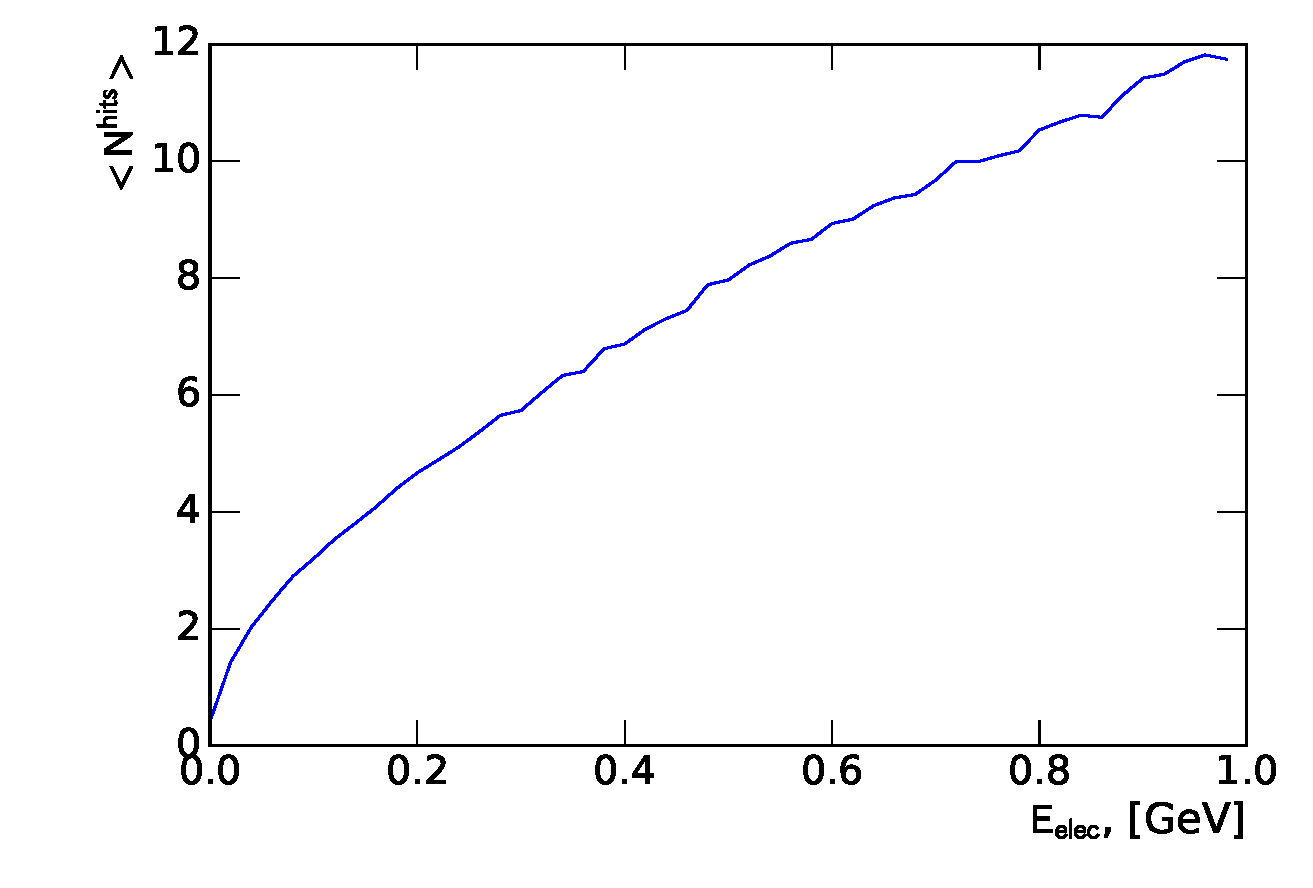
\includegraphics[width=1.0\linewidth]{MC/nHitsMean.pdf} \\ b)}
\end{minipage}
\caption{Distribution  of the a) electron energies and b) mean number of hits in the shower vs energy of electron for electrons with energy less than 1 GeV originating from 1 TeV initial electron.}
\label{fig:TrackEnergy}
\end{figure}

The fast simulation of  the forward calorimeters is a complicated task due to their complex structure. As it was mentioned in Sec.~\ref{sec:forwardCalo} FCAL consists of hexagonal absorber cells with an anode tube and cathod rod in the cell center and the liquid argon in the gap between rod and tube. In order to simulate the resolution of high-energy electrons, an efficient fast simulation technique should take into account this large amount of non-uniformly distributed sensitive material.

The electron energy resolution for this calorimeter can be written as:
\begin{equation}\label{eq:EMResoultion}
\frac{\sigma}{E} \approx \frac{1}{\sqrt{E}}	\oplus \frac{1}{E} 	\oplus const,
\end{equation}
where $\oplus$ indicates the quadratic sum. The first term is the 'stocastic term', which includes intrinsic shower fluctuations, the second  one takes into account readout noise effects and pile-up fluctuations. The constant term is connected to non-uniformities in the detector, causing large fluctuations of the energy loss. The energy resolution of high-energy electrons is mostly dominated by the constant term. 

Fluctuations due to the detector design are visible in the simulation of low energy electrons, generated inside different points in the forward calorimeter. The shower energy $E^{shower}$ distribution in the transverse x vs y plane is shown on Fig.~\ref{fig:FSFluctuations} a). The shower energy is defined as:
\begin{equation}
E^{shower}=\sum E_i^{hits},
\end{equation}
where $E_i^{hits}$ is the energy of the i-th hit in shower shower inside the sensitive material. The periodic structure resembles the calorimeter design, where the light circles correspond to gaps with liquid argon, which are acting as sensitive material. Introduction of distance to the closest rod center, calculated as shown in Fig.~\ref{fig:FSFluctuations} b) allows to catch this periodic structure.

A typical electron substituted by frozen shower coming from simulation of high-energy electrons has a relatively small energy (Fig.~\ref{fig:TrackEnergy} a). The mean number of deposits in the sensitive material in a "frozen" shower is around 5 and this value rises with the electron energy (Fig.~\ref{fig:TrackEnergy} b).  Fig.~\ref{fig:FSProduction} presents the distribution of the distance to a closest rod center vs shower energy for showers from electrons with energy below 1 GeV originating from initial electrons with an energy of 1 TeV. The liquid argon gap is marked by red lines. There is visible peak in showers energies for the region around liquid argon gap. The similar structure is also visible in a number of hits  (Fig. ~\ref{fig:ShowerProp} a) and the standard deviation of energy of the hits in the shower (Fig. ~\ref{fig:ShowerProp} b) distributions. The magnitude of the peak depend on the electron energy and is higher for the low energies (Fig. ~\ref{fig:FSProduction2} a) and less significant for higher energies (Fig. ~\ref{fig:FSProduction2} b).  This fact combined with energy distribution states the importance of a proper simulation of non-uniformities for showers coming from a low energy electrons.





\begin{figure}[!tbp]
\center{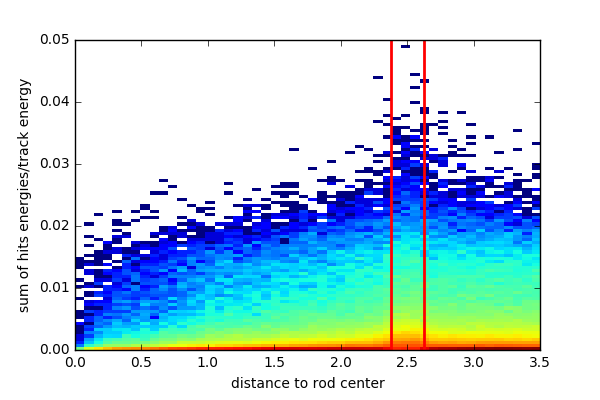
\includegraphics[width=1.\linewidth]{MC/fullBinningScatter.png} }
\caption{Distribution of distance to the closest rod center vs shower energy for electron showers created by electrons with energy less than 1 GeV originating from the initial electrons with energy 1 TeV in distance to the closest rod center vs shower energy plane. Position of the liquid argon gap is noted by a red lines. }
\label{fig:FSProduction}
\end{figure}

\begin{figure}[!tbp]
\begin{minipage}[h]{0.49\linewidth}
\center{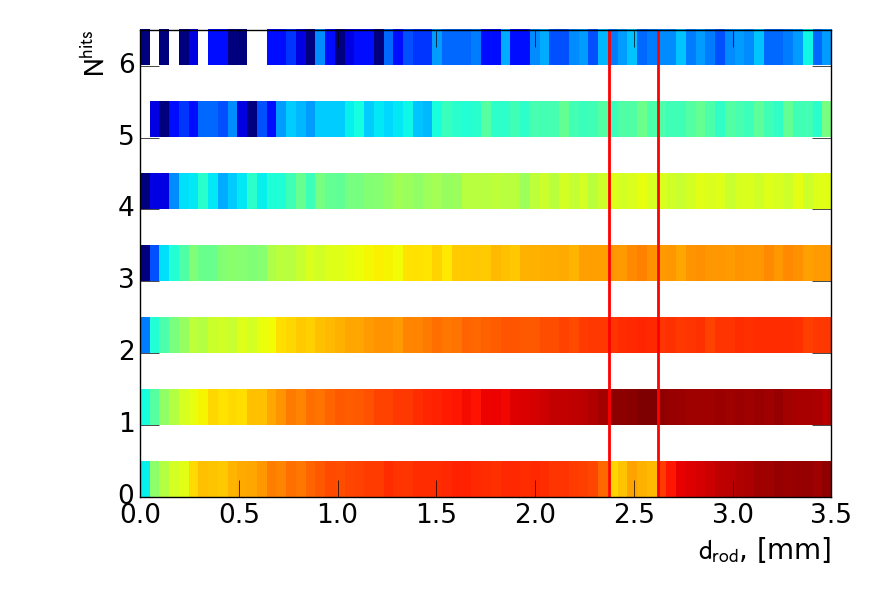
\includegraphics[width=1.0\linewidth]{MC/nHits.png}  \\ a)}
\end{minipage}
\hfill
\begin{minipage}[h]{0.49\linewidth}
\center{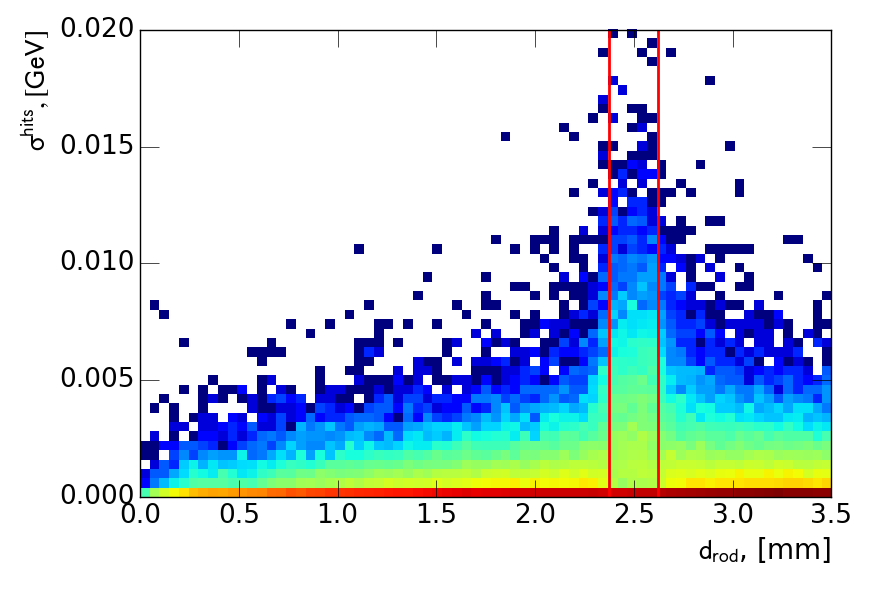
\includegraphics[width=1.0\linewidth]{MC/rms.png} \\ b)}
\end{minipage}
\caption{Distribution of distance to a closest rod center vs a) number of hits in a shower plane and b) standard deviation of hits in a shower energy of electron showers created by electrons with energy less than 1 GeV coming from initial electron with energy 1 TeV. Position of a liquid argon gap is noted by a red lines.}
\label{fig:ShowerProp}
\end{figure}

\begin{figure}[!tbp]
\begin{minipage}[h]{0.49\linewidth}
\center{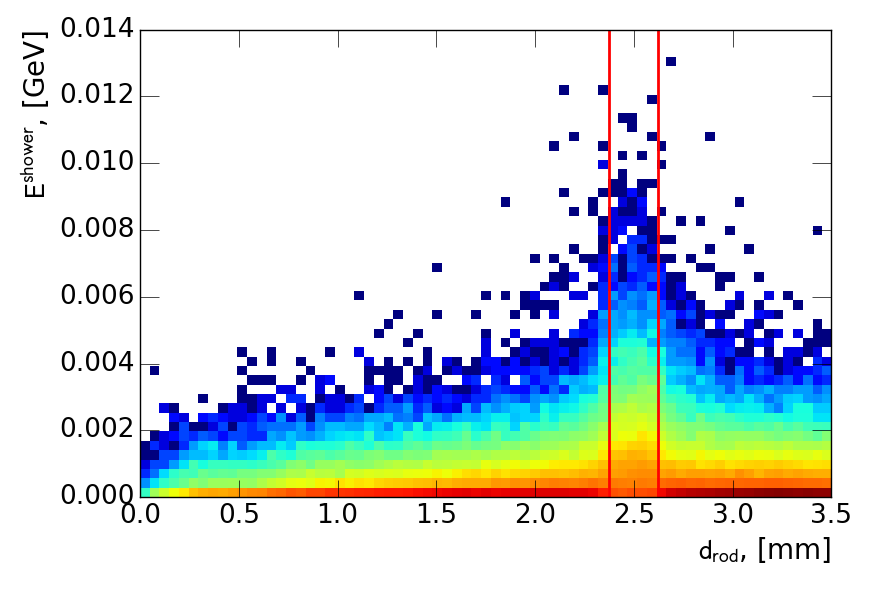
\includegraphics[width=1.\linewidth]{MC/fullBinningScatterSmall.png} \\ a)}
\end{minipage}
\hfill
\begin{minipage}[h]{0.49\linewidth}
\center{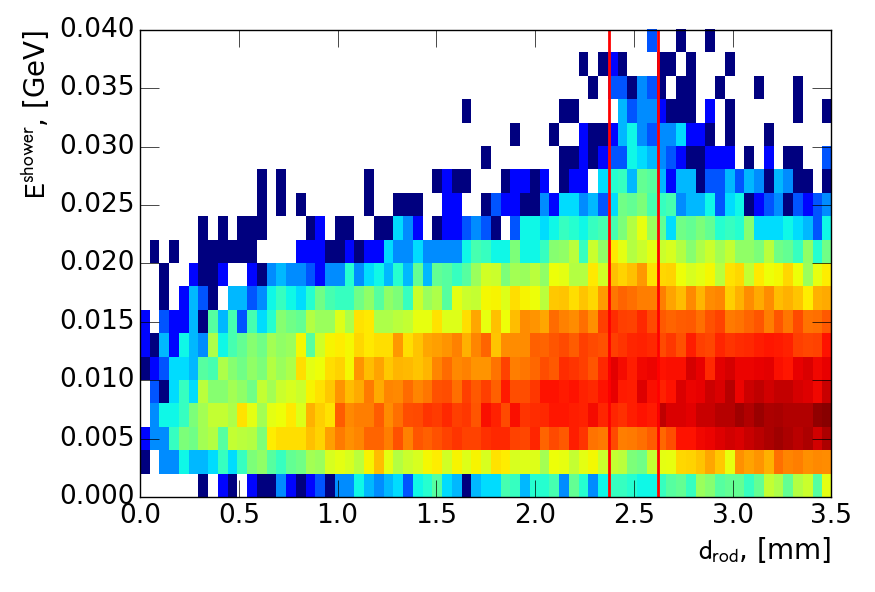
\includegraphics[width=1.\linewidth]{MC/fullBinningScatterBig.png} \\ b)}
\end{minipage}
\caption{Distribution of distance to a closest rod center vs shower energy for electron showers created by electrons with energy a) less than 100 MeV  and b) higher than 300 GeV coming from initial electron with energy 1 TeV in  plane. Position of a liquid argon gap is noted by red lines. }
\label{fig:FSProduction2}
\end{figure}

On the another hand, the use of the frozen showers in too low energy region can be suboptimal because of the small number of energy depositions in a shower. For electrons with energies below 30 MeV 90\% of the showers have no depositions and only 0.5\% of showers have more than 1 hit (Fig.~\ref{fig:fracHits}). It was figured out, that below this energy, the substitution of the electron by the single hit with electron energy have showed a faster speed of simulation.

\begin{figure}[!tbp]
\begin{minipage}[h]{0.49\linewidth}
\center{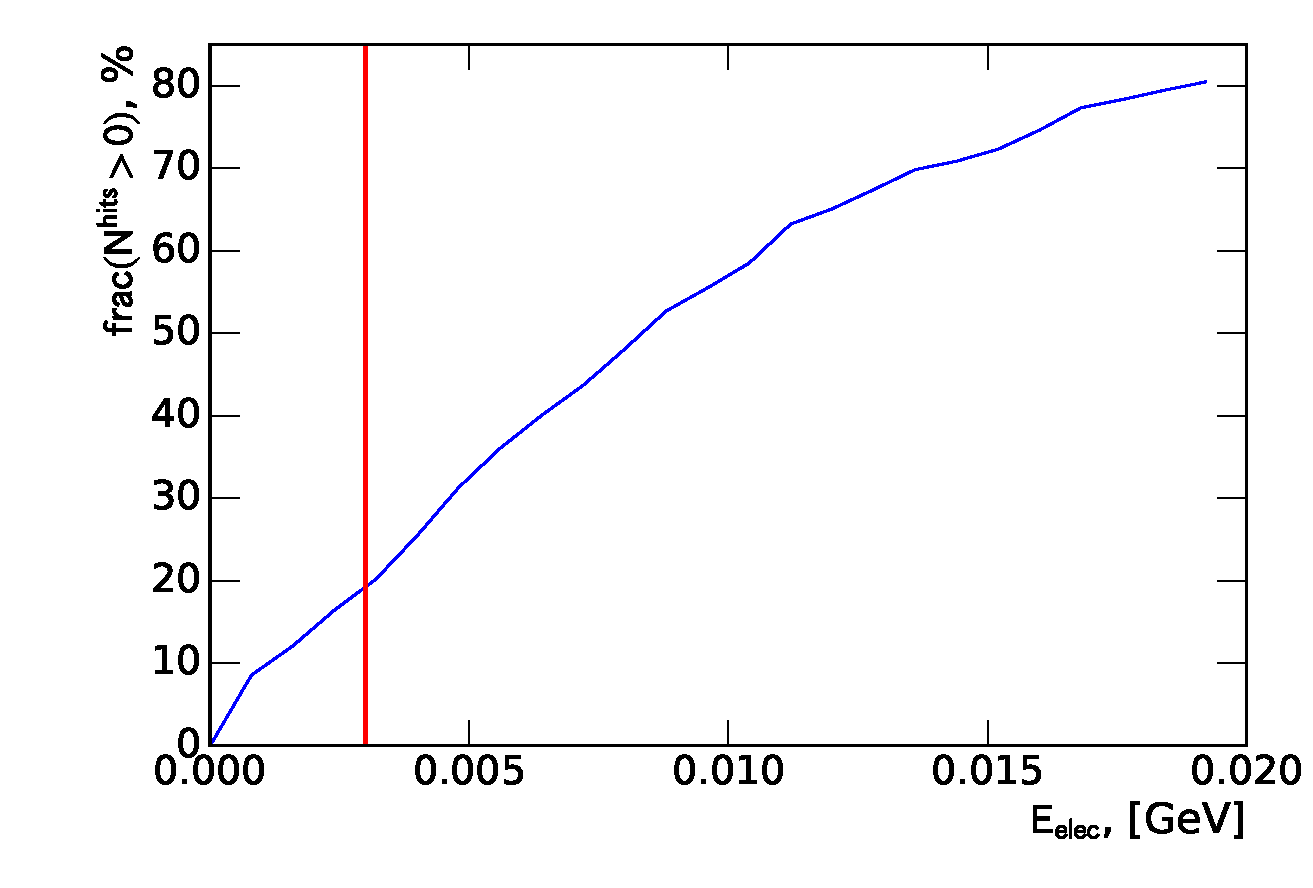
\includegraphics[width=1.\linewidth]{MC/fracHits2.pdf} \\ a)}
\end{minipage}
\hfill
\begin{minipage}[h]{0.49\linewidth}
\center{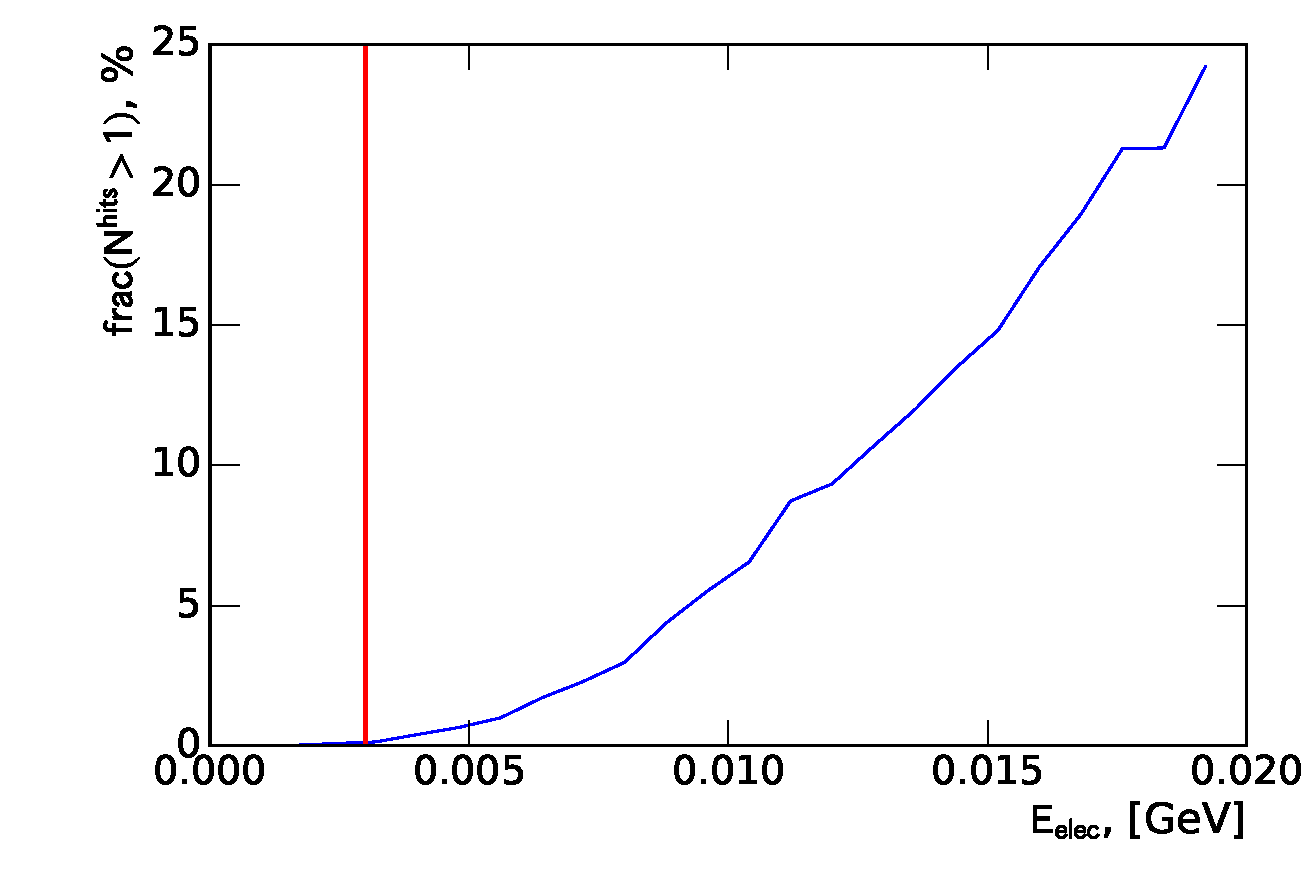
\includegraphics[width=1.\linewidth]{MC/fracHits.pdf} \\ b)}
\end{minipage}
\caption{Fraction of showers with a) at least 1 b) at least 2 depositions inside the sensitive material depending on the initial electron energy. The red line denotes the 30 MeV limit for the frozen showers method.}
\label{fig:fracHits}
\end{figure}


\section{Generation and use in simulation}\label{sec:FSProdUse}

As it was mentioned in the introduction, the frozen showers method consist of two stages: generation of libraries and the use in simulation. The generation needs to be repeated for each significant change in the physics processes description of Geant4 or in the description of the detector. Showers are stored in a library in bins of pseudorapidity and distance to the closest rod center, while the energy remains unbinned. There is special \textit{liquid argon bin} for distance with position and width, that corresponds to the parameters of liquid argon gap, that was introduced in order to catch non-uniformities form Sec.~\ref{sec:FSproblem}.

In order to obtain a proper energy distribution for the generation of the library, particles originating from SM process ($t\bar{t}$ or high energy electrons) are usually used. For each particle eligible for frozen showers use parameters are saved for a later use. On a second stage, these particles are propagated through the calorimeter using full \atlas simulation infrastructure. Each hit is saved as a shower inside the library in a corresponding pseudorapidity and distance bin. 

Additionally, in order to save disk space as well as a memory consumption, the hit information is compressed. This compression is performed in two steps: 
\begin{description}
\item [Hit merging] If the distance between any two hits is smaller, than a given parameter $R_{min}$, then these hits are merged into one deposit at the energy weighted center of them. This process is done iterativelly.
\item [Truncation] Hits which energies are below a fixed fraction $f$ of the total energy sum of all hits, are truncated. The energy of the remaining hits is rescaled in order to preserve the total deposited energy.
\end{description}

During simulation, if the energy of a particle falls below a cut-off energy, the FS algorithm examines the resulting shower. It checks whether the particle is far from the edges of the calorimeter, such that the  shower is by 90\% contained inside the calorimeter. This depends also on the energy of the particle, since the  shower sizes are increasingly growing with energy. The algorithm searches for a shower with the closest energy in the corresponding pseudorapidity and distance bins. The shower is rotated in the direction of the particle. In order to correct for the differences in the energy, each hit in the shower is scaled as:
\begin{equation}
E_{hit}^{new}=E_{hit}\cdot \frac{E_{part}}{E_{part,lib}},
\end{equation}
where $E_{hit}$ is the original energy of the hit, $E_{part}$ is the energy of the particle and $E_{part,lib}$ is the energy of the particle from the library. Afterwards particle is substituted by the resulting shower. Later, the reconstruction algorithm uses these hits from the frozen shower as usual energy deposits in the sensitive material. 

\begin{figure}[!tbp]
\center{
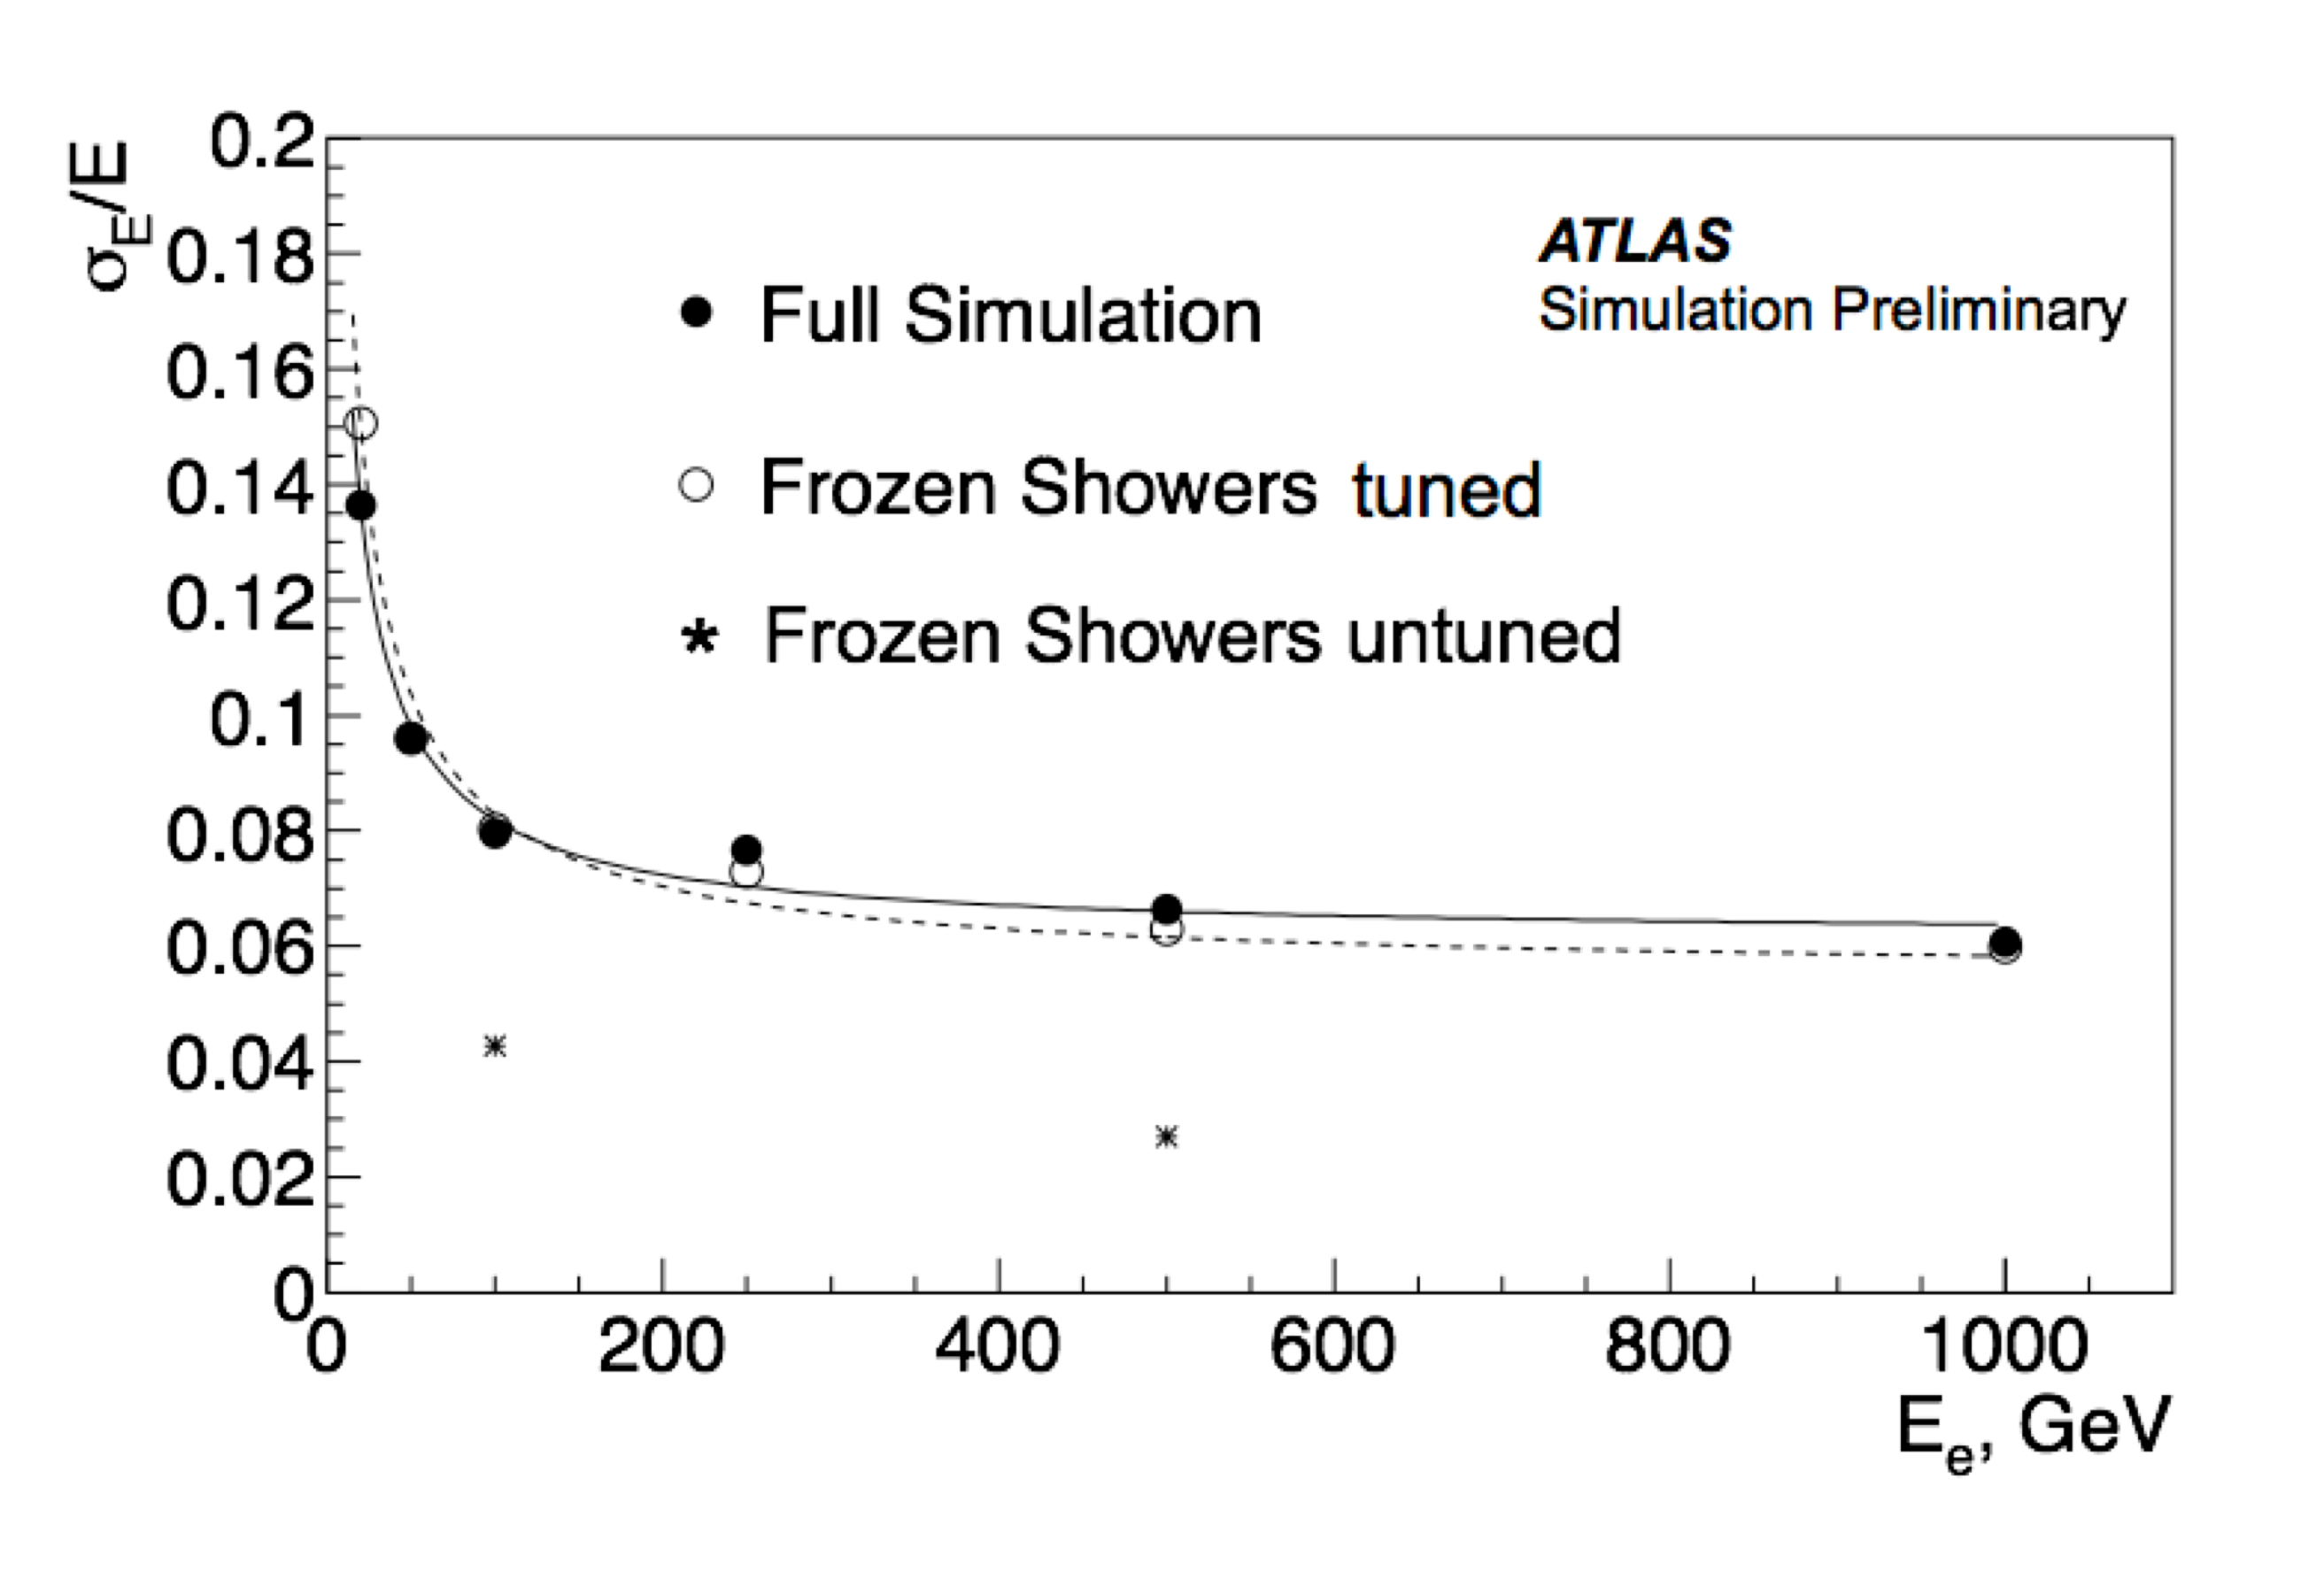
\includegraphics[width=0.8\textwidth]{MC/fs.png}
\caption{Electron resolutions for full simulation(black dots), tuned(white circles) and untuned(star points) frozen showers. Electrons simulated with frozen showers libraries before tuning have twice smaller resolution, than electrons from full simulation. Tuning allows to gain better agreement with full simulation.}
\label{fig:FS_resolution}}
\end{figure}

\begin{figure}[!tbp]
\center{
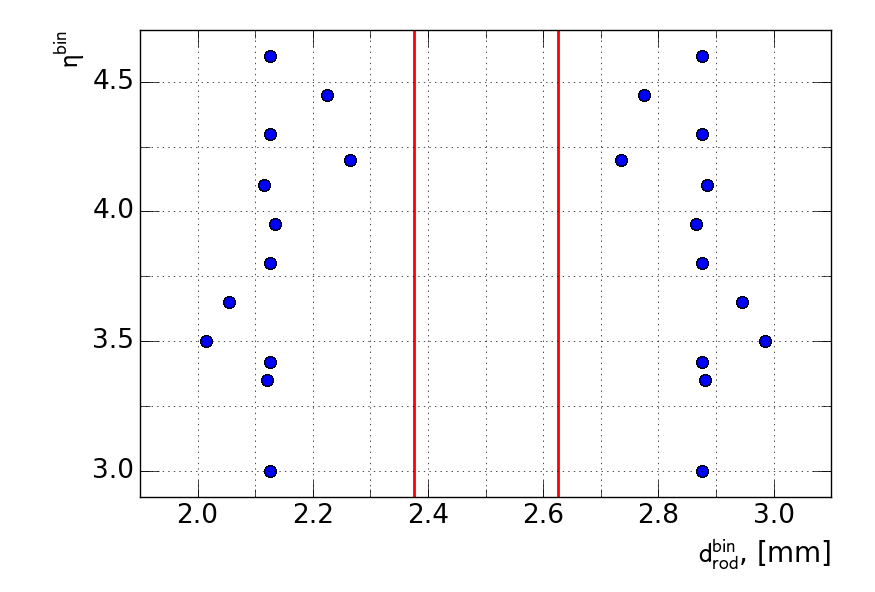
\includegraphics[width=0.8\textwidth]{MC/oldTuning.png}
\caption{Position of gap bins for different $\eta$ bins in the previous libraries after tuning. The dots correspond to the limits of each bin. The red lines are denoting the original position of the bins, which correspond to the position of the liquid argon gap in the calorimeter.}
\label{fig:FSOldTuning}}
\end{figure}

\subsection{Tuning of libraries-}\label{sec:LibTuning}

The good simulation method is required to be consistent with full simulation on all possible reconstucted objects. In case of Frozen Showers in forward calorimeter, the electron energy resolution is the most problematic value, since the resolution of the reconstructed electrons is around 2 times smaller(Fig.~\ref{fig:FS_resolution}), than in the full simulation. Using the Eq.~\ref{eq:EMResoultion}, this behavior can be interpreted as a smaller size of fluctuations for fast simulation and therefore lack of the high-energy showers originating in sensitive matrial. This problem can be solved by tuning the parameters of library in order to match the full simulation.

The tuning consists of a 2-step manual procedure:
\begin{description}
\item [Changing bin width] At this stage position of the liquid argon bin is moved, so what a bid width is enlarged. This causes a higher number of showers with higher response in simulation and therefore higher fluctuations. This procedure causes a higher resolution and a mean energy of reconstructed electrons.
\item [Shower energy scaling] In order to correct for the introduced shift in the energy scale, the shower energy is reduced by rescaling all the hits in the shower to the shift in the mean reconstructed energy.
\end{description}
 It is repeated iterativelly in each pseudorapidity bin separately untill the desired agreement is obtained. The resulting bin positions are shown on a Fig.~\ref{fig:FSOldTuning}. This method yields a relatively good agreement with full simulation (black dots on Fig.~\ref{fig:FS_resolution}). However, it is necessary to repeat this procedure for each new library generation and this requires a significant tuning effort, which makes it not optimal. 

\section{Machine learning based bin finding procedure}\label{sec:MLBinning}

Since frozen showers were planned to be used in the Run-2 Monte Carlo production, there was a need for a more automatic procedure of library generation with proper electron resolution. One of the possible ways is to choose the different positions of liquid argon bins during library generation using machine learning tools. In this section a newly developed automatic bin finding procedure will be discussed.

\subsection{Machine learning introduction} 

Machine learning is a set of algorithms, which allows algorithms to learn and improve from experience without being explicitly programmed. This is a modern field of computer science, that is used in different fields like computer vision, natural language processing, data science etc. There are two main types of machine learning algorithms: \textit{supervised}, where a example of the desired output is provided by the "supervisor" and the goal is to learn a general rule, that maps inputs to outputs, and \textit{unsupervised} learning, where no labels are given to the algorithm, which discovers the hidden patterns in the data\cite{0070428077}. The initial data parameters of interest, which are used in the algorithm to "learn" are called \textit{features}. 

Machine learning algorithms can be used for solving a classification problem, where each event should be identified to one of the specified classes. Since the first introduction of machine learning classifying algorithms called perceptron by Rosenblatt\cite{VanDerMalsburg1986}, many different algorithms have been invented. In this analysis, decision trees and support vector machines implemented in Scikit-Learn python package\cite{scikit-learn} are used. 

\subsubsection{Binary decision trees}

\textit{Binary decision trees}\cite{cart84-2}, called also single decision trees, are one of the most commonly used machine learning algorithms for a classification problems in particle physics. It can be represented as a set of sequential cuts on input variables. 
Scheme of this algorithm is shown in Fig.~\ref{fig:MLAlgo} a). Red circles show the nodes of the tree. Each node corresponds to the one of the internal input variables and connects to two branches, that are split in the respect to the value. The first node is called a root node. The depth of the tree is the number of branches from the node to the tree's root node. The tree ends with squares, called leaf nodes, where all events are classified to a certain class. Leaf node represents classification or decision. The tree, where each node has at most 2 children called binary decision tree.

The tree is build using the variable called Shannon entropy\cite{ShannonEntropy}, what is similar to the entropy in physics:
\begin{equation}
S=- \sum_{i=1}^{N} p_i log_2 p_i,
\end{equation}
where $p_i$ is the probability to find event of class i. Each split in a variable should decrease the entropy of the system. The information gain is defined as the difference in entropy after the split:
\begin{equation}
IG(Q) = S_0 - \sum_{i=1}^{2}S_i,
\end{equation}
where $S_0$ is the initial entropy, without new node, $S_i$ is the entropy of the one of the 2 node children. The node with the highest information gain is taken. One of the main advantages of the decision trees its simplicity of visualization and interpretation. 

\subsubsection{Support vector machines}

\begin{figure}[!tbp]
\begin{minipage}[h]{0.49\linewidth}
\center{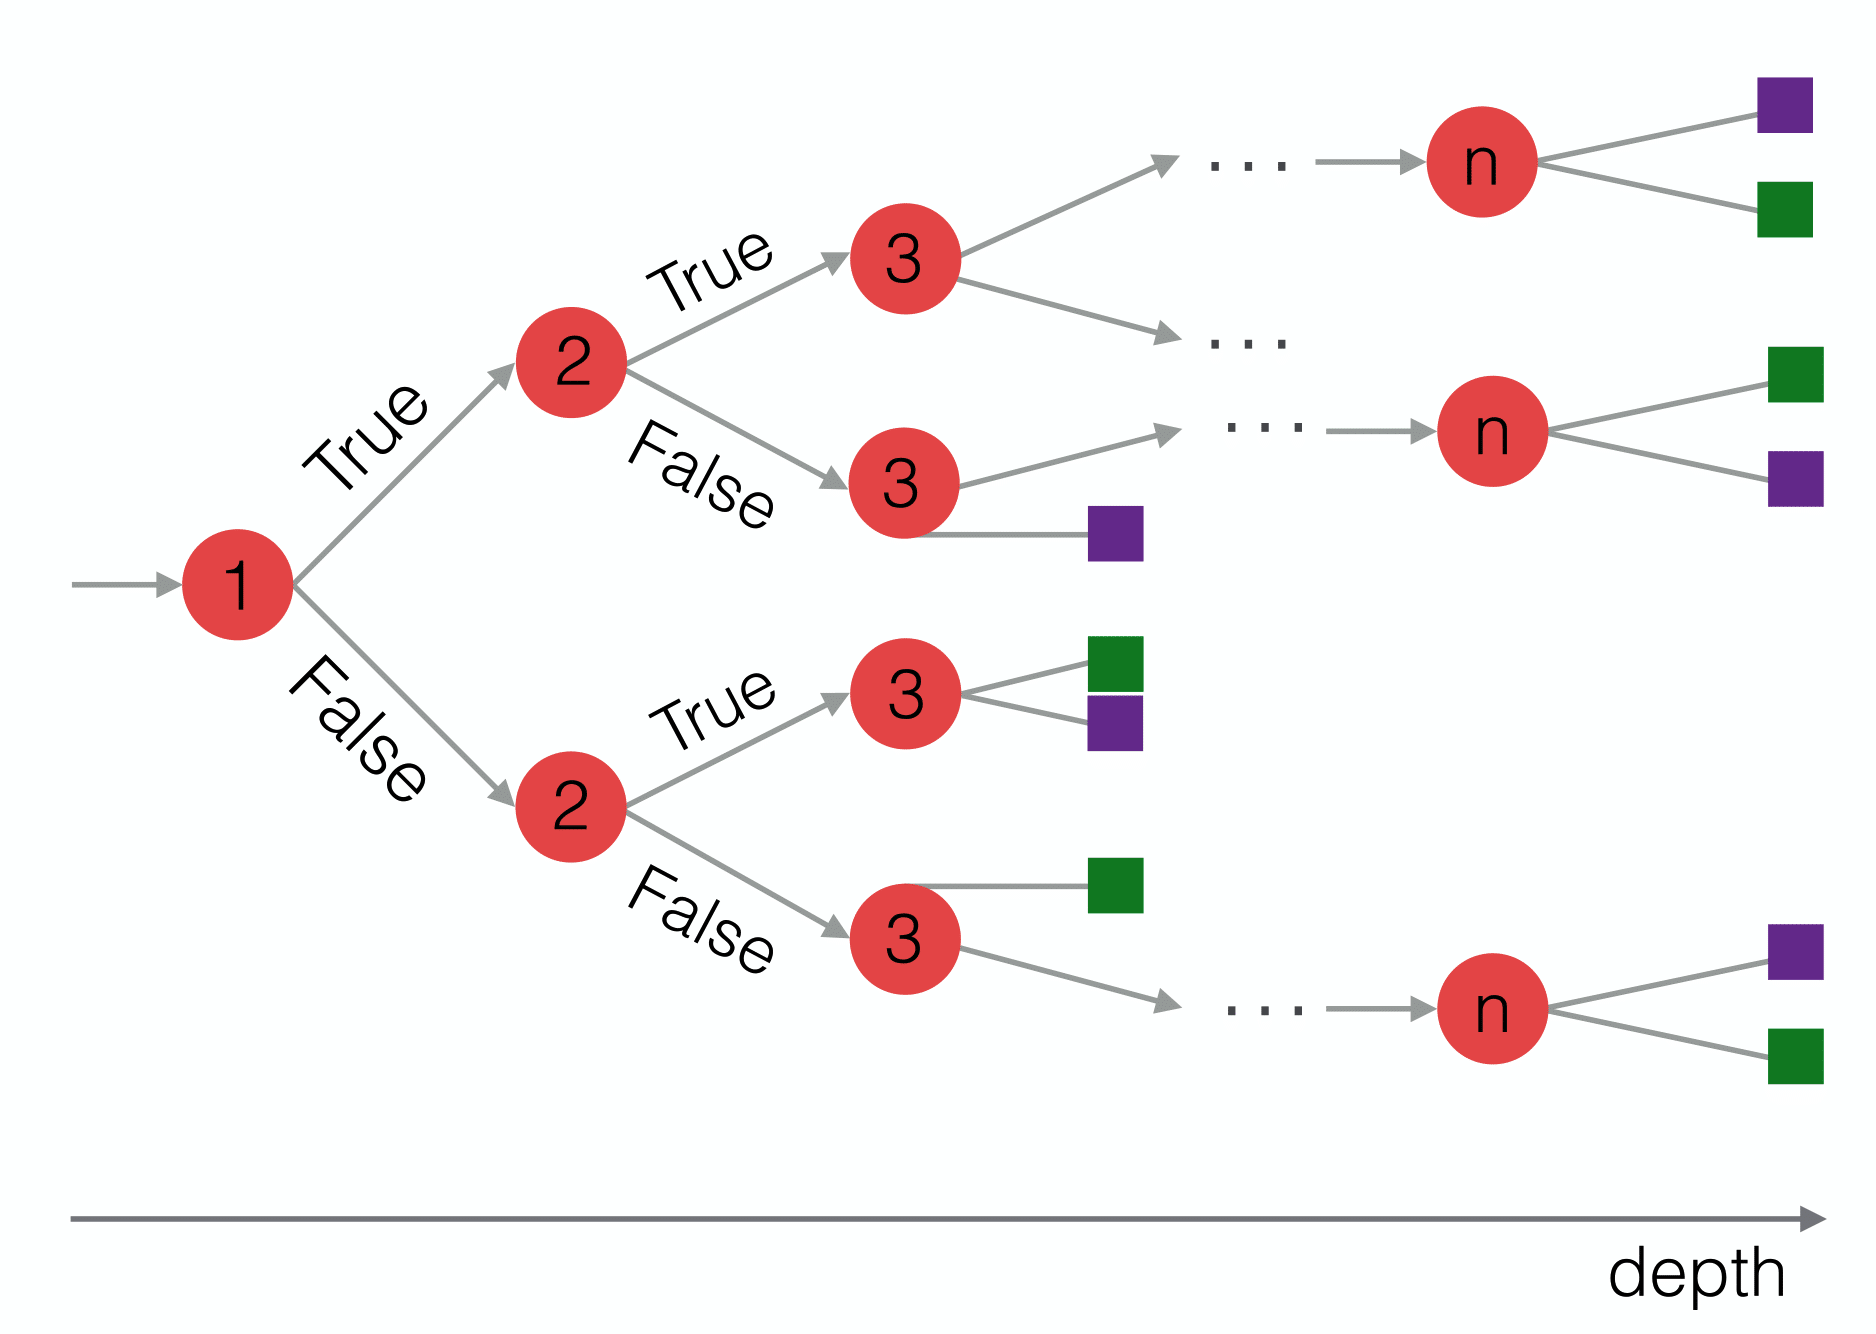
\includegraphics[width=1.\linewidth]{MC/DecisionTree.png} \\ a)}
\end{minipage}
\hfill
\begin{minipage}[h]{0.49\linewidth}
\center{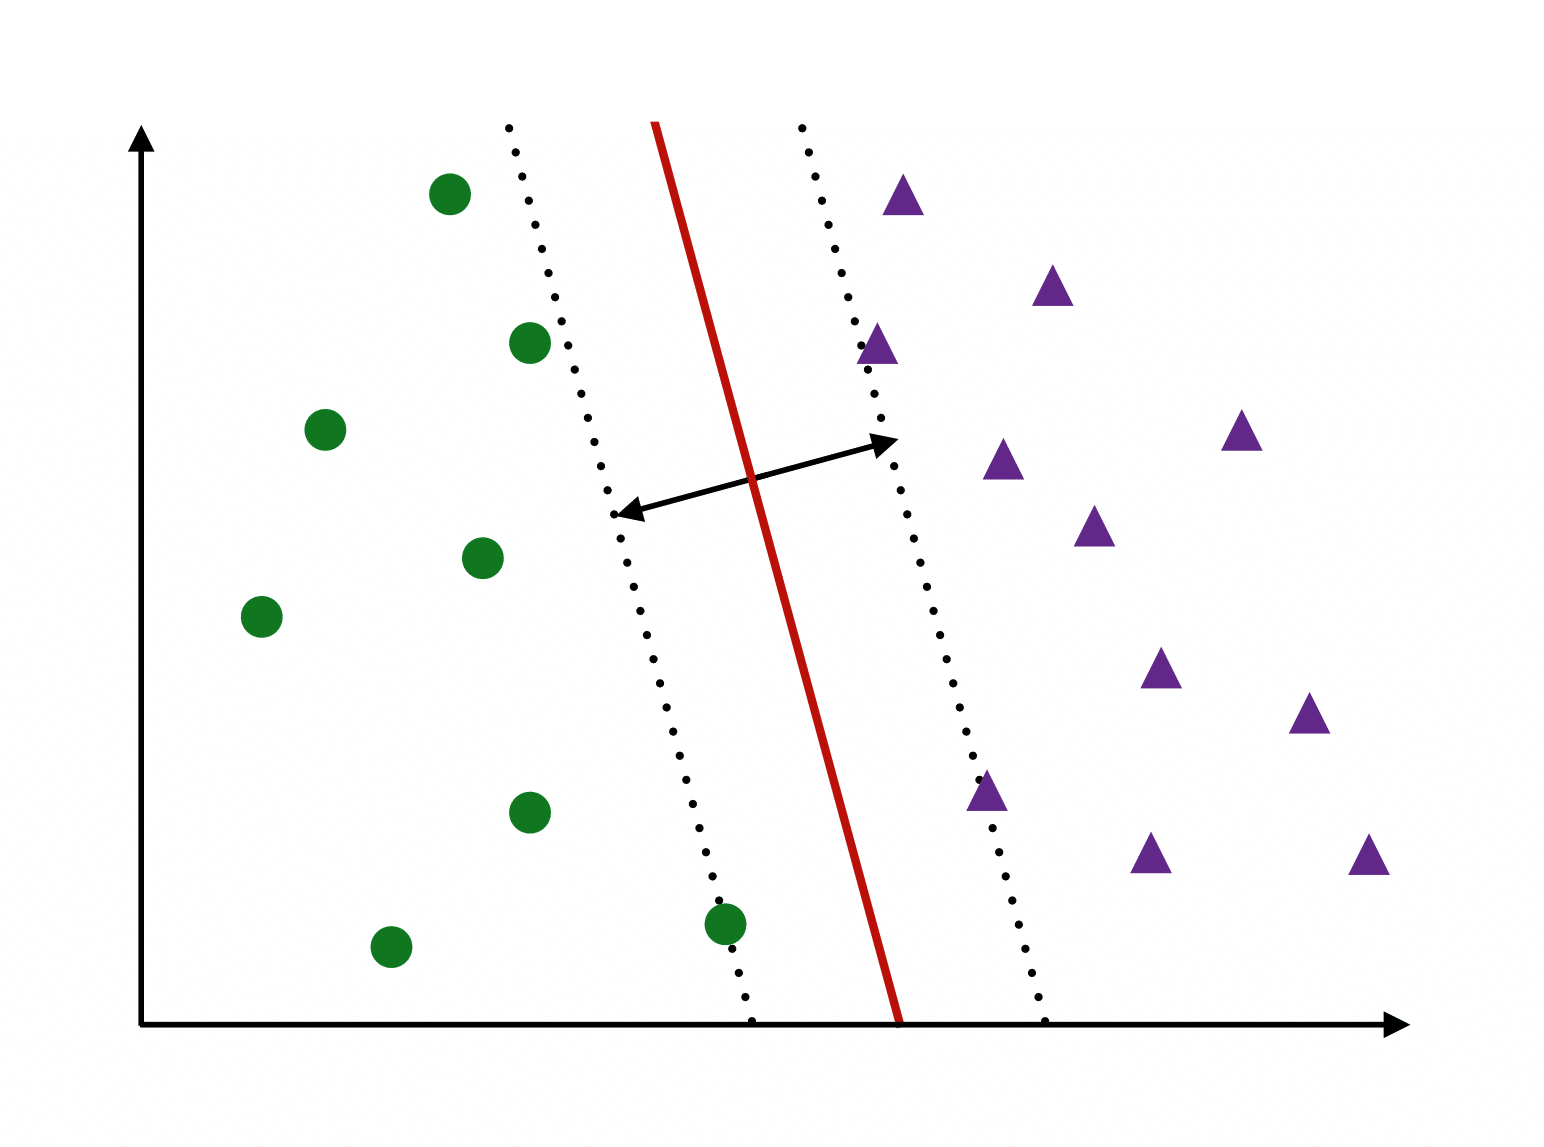
\includegraphics[width=1.\linewidth]{MC/SVM.png} \\ b)}
\end{minipage}
\caption{Schematic representation of machine learning algorithms, used in this analysis for the classification of showers. Green figures represent the first class of events, whereas violet ones belong to a second class.  
a) Representation of a binary decision tree structure: red circles correspond to nodes, which are split with the respect to the selected feature. Squares represent leafs, where events classified to a certain class. The depth of the tree is calculated as a maximum number of edges from the node or leaf to the root node. 
b) Representation of the SVM algorithm. The dividing hyperplane is shown by the solid line. The dashed lines represent the maximum margin boundaries.}
\label{fig:MLAlgo}
\end{figure}

\textit{Support vector machines} (SVM) is a supervised machine learning algorithm which can be used for classification problems\cite{VapLer63}. In this algorithm each event is represented in a p-dimensional parameter space. The classification is performed by finding hyper-plane that differentiates given two classes with the largest possible separation (Fig. ~\ref{fig:MLAlgo} b). The hyperplane can be described with the set of points $\vec {x}$ in the parameter space satisfying:
\begin{equation}
\vec{w}\cdot \vec{x} - b = 0,
\end{equation}
where $\vec{w}$ is the normal vector to the hyperplane and the parameter $\frac {b}{\|{\vec {w}}\|}$ determines the offset of the hyperplane from the origin along the normal vector $\vec {w}$. 

The maximum margin boundaries are described by equations:
\begin{eqnarray}
\vec{w}\cdot \vec{x} - b = 1, \\
\vec{w}\cdot \vec{x} - b = -1,
\end{eqnarray}
where $\frac{2}{\|\vec{w}\|}$ is the distance between these 2 hyperplanes, such that the planes with the maximum margin between them should have  minimum $\|\vec{w}\|$. 

In order to prevent each point from falling into the margin, the following constrain should be satisfied: 
\begin{eqnarray}
\vec{w}\cdot \vec{x} - b \geqslant 1 \textrm{ where } y_i = 1,\\
\vec{w}\cdot \vec{x} - b \leqslant -1 \textrm{ where } y_i = -1,
\end{eqnarray}
where $y_i$ represents the class of the i-th event, that can be either 1 or -1. These equations can be rewritten as:
\begin{equation}
y_i(\vec{w}\cdot \vec{x} - b ) \geqslant 1
\end{equation}

It is also possible to construct a non-linear classifier by replacing the dot-product with a different kernel function. In this thesis, a radial basis function (RBF) kernel is used:
\begin{equation}\label{eq:RBF}
K_{rbf}(\vec{x}_i, \vec{x}_j) = e^{-\gamma | \vec{x}_i - \vec{x}_j|^2} \, \gamma >0,
\end{equation}
where the parameter $\gamma$ adjusts the width of the kernel.




\subsection{Electron shower categorization}

\begin{figure}[!tbp]
\center{
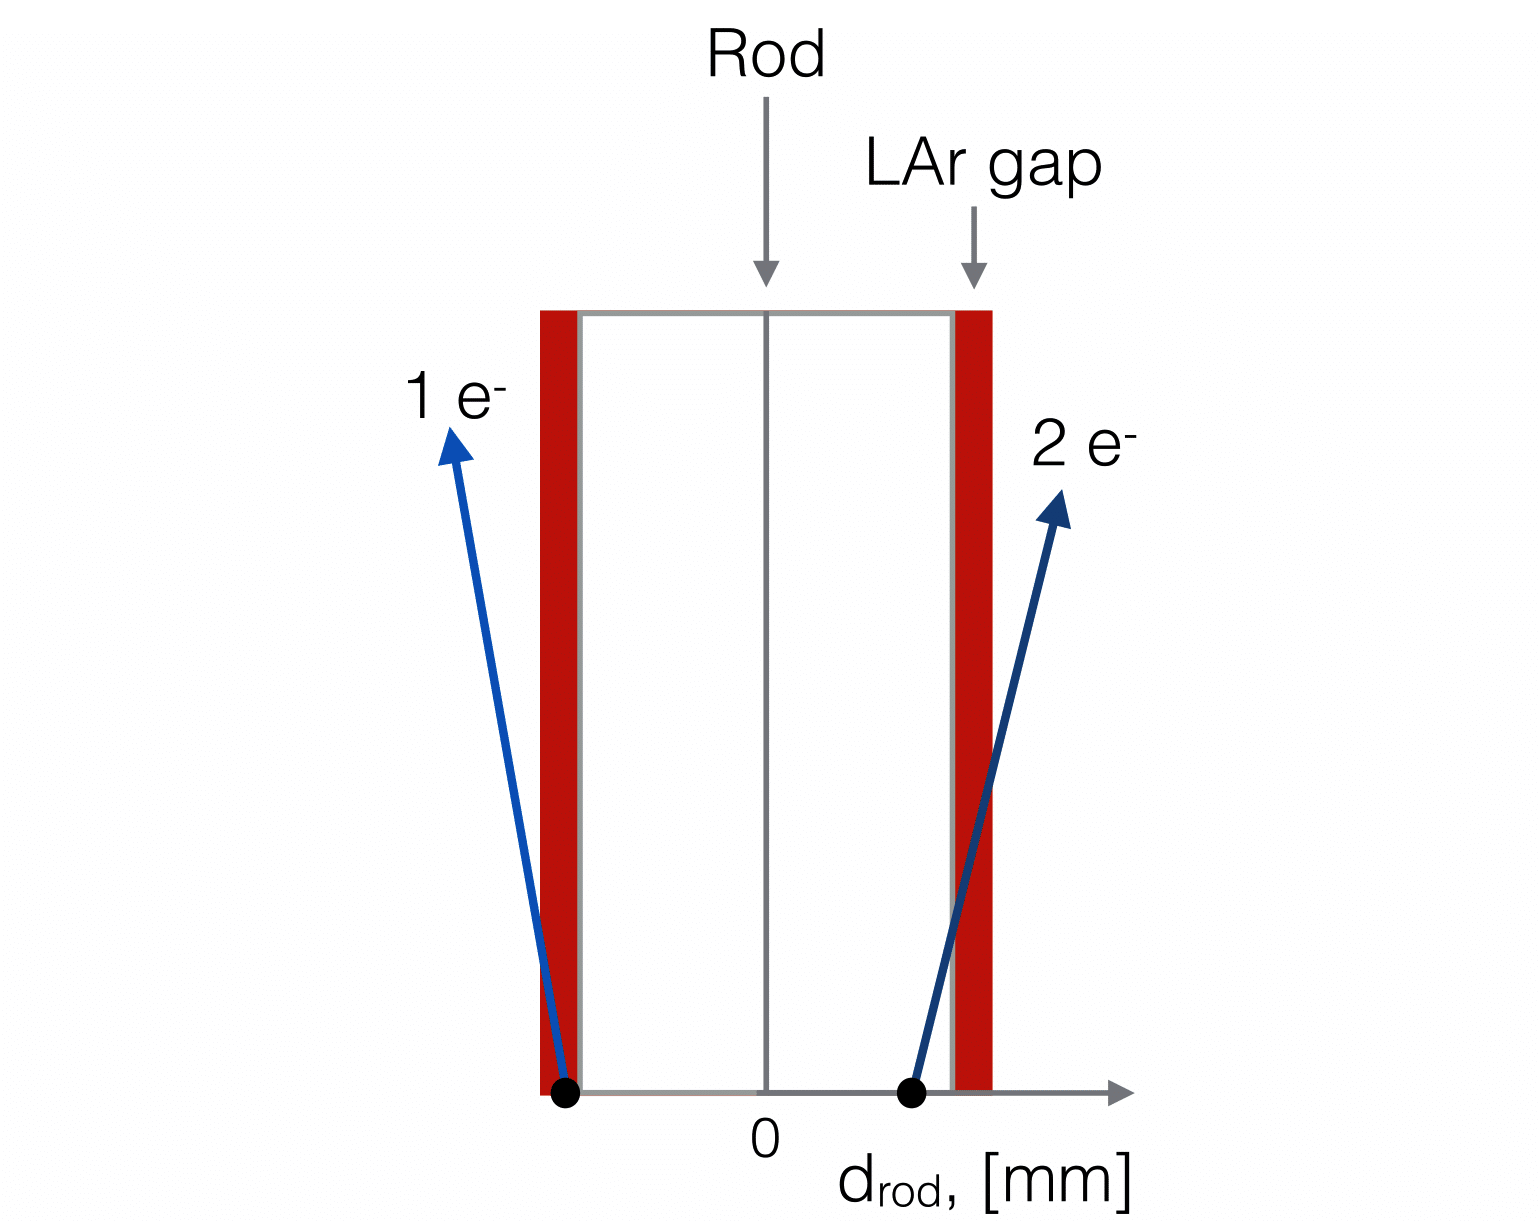
\includegraphics[width=0.5\textwidth]{MC/Model2.png}
\caption{Schematic representation of the model of shower creation in the FCAL. Electron 1 is created in a liquid argon gap. Electron 2 is created near a liquid argon gap and crosses it. This causes a smearing of sensitive material showers distribution. Electrons created in the sensitive material tend to create more energetic showers, than electrons from the dead material. However, electrons shown on this scheme may give similar showers and therefore may not be distinguishable.}
\label{fig:Model}}
\end{figure}

As it was mentioned in the previous sections, the FCAL modules consist of different types of material such that showers starting inside the dead material are usually having lower energies, than those started in sensitive material. However, the validation (Fig.~\ref{fig:FS_resolution}) can be interpreted as an implication that there are high-energy showers outside the liquid argon gap. It could be explained by the fact, that electrons, created in a dead material, can cross a liquid argon gap and give a hit there as shown in Fig.~\ref{fig:Model} (electron 2). These electrons would be indistinguishable from electrons created directly in the sensitive material (electron 1 in Fig. \ref{fig:Model}). 

Due to this similarity, electrons created outside the sensitive material can be treated together, labelling such showers \textit{sensitive matrial showers}. Showers that did not cross a liquid argon gap, are called dead material showers. This means, that in this model a real liquid argon gap can be substituted by the "effective" one, with larger width.

The width of the effective liquid argon gap, from the definition, depends on the following parameters:
\begin{description}

\item [Electron energy] The gap should get wider with higher energy of the initial electron, because of the growth of the mean free path with energy.
\item [Direction of the electron] Electrons aligned collinearly with the liquid argon gap will have smaller probability to cross it. This probability will grow with the angle reaching its maximum at  $90^{\circ}$

\end{description}

The bin finding is performed as a 2-step procedure:  on the first stage the first classifier distinguish the showers based on their simulated parameters and on the second step the second classifier aims to produce a hyperplane in $d_{rod}$, $E$ of initial electron phase-space. This classifiers and the training sample used will be discussed in details in the following subsections.

\subsubsection{Training sample}

Real distributions of parameters of electrons, used in simulation, have a complicated structure and depend on the physics processes simulated. Machine learning could identify these dependencies instead of the needed ones. This is why a simplified data is needed as a training sample for machine learning. The training sample was produced by simulation of electrons directly in the forward calorimeters. In order to treat equally high and low energy electron initial showers, a uniform energy distribution is used.

Fig.~\ref{fig:EtaMomVsEnergy} shows the distribution of the shower direction ($\eta^{direction}$) vs electron energy for electrons coming from simulation of 1 TeV electron. Most of the showers have direction in $\eta$ range between 3.0 and 5.0, which corresponds to position of the FCAL. It was figured out, that the direction of the shower is highly correlated with the postion of the electron. Therefore, electrons were generated uniformly in $\eta$ between 3.0 and 5.0.


\begin{figure}[!tbp]
\center{
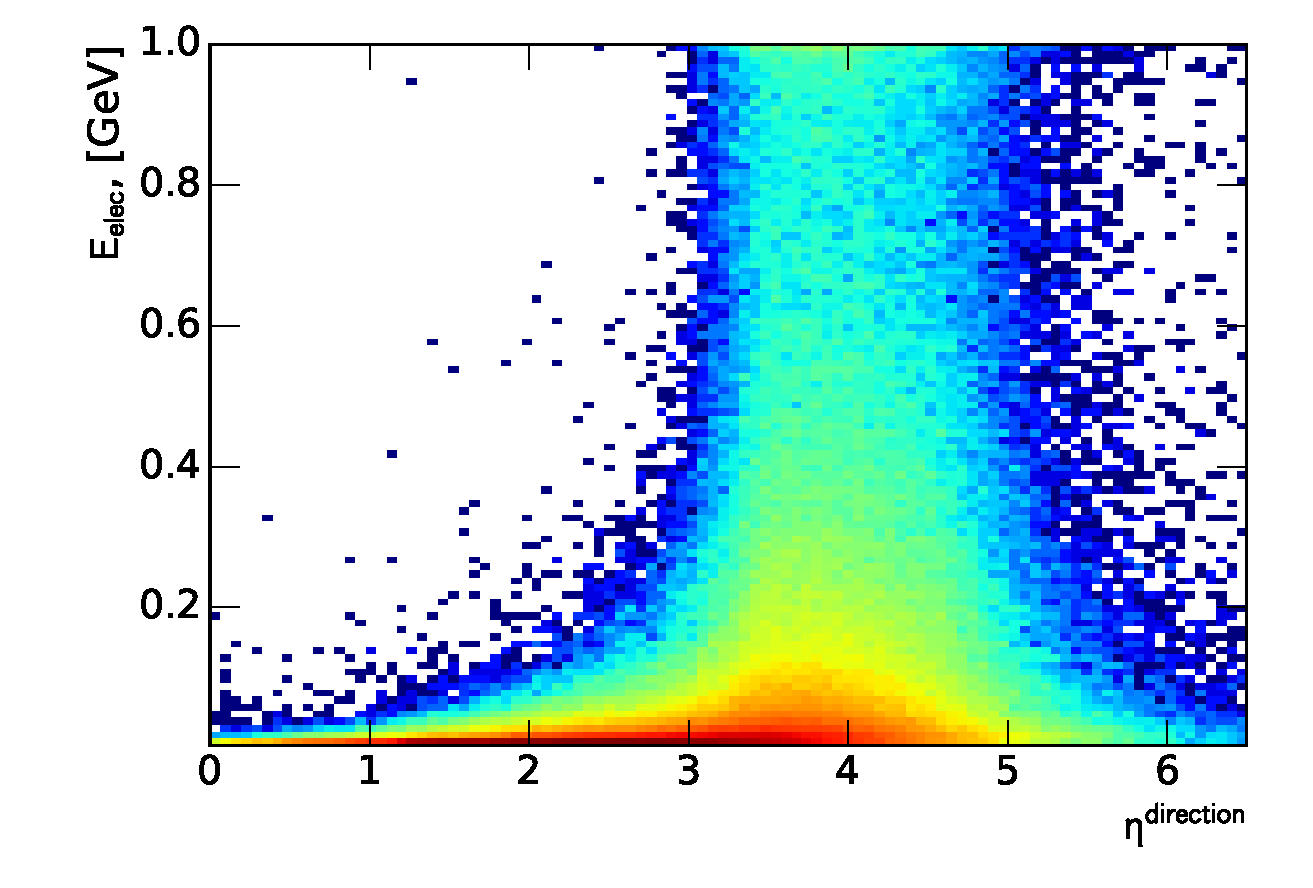
\includegraphics[width=0.8\textwidth]{MC/FSEtaMomVsEnergy.pdf}
\caption{Distribution of sub-showers energy vs direction of shower $\eta_{momentum}$ for showers from the production of 1000 GeV electrons.}
\label{fig:EtaMomVsEnergy}}
\end{figure}

\subsubsection{First classifier}

The first classifier aims to categorize all showers by means their parameters. An supervised learning algorithm is used on artificially reduced training sample, where the labels can be put automatically. The obtained classifier is later expand the classification to the full training sample. 

Pre-labeling is done using the definitions of sensitive and dead material showers based on the distance to a closest rod center (Fig.~\ref{fig:SchemePresel}). Showers starting in a liquid argon gap are defined as sensitive material showers, while showers coming from electrons born near the rod center and on the edges of the cells can be labeled as dead material showers, since there is a small probability for the electron, which caused the shower, to reach the liquid argon gap.

For this classifier a simple decision trees have been chosen, since it has showed a good classification efficiency on the reduced training sample. Different input parameters have been tested using their variance, and it was figured out, that the best set of the differentiating parameters is:

\begin{itemize}
\item Shower energy, defined as the sum of all sensitive material hits energies in the shower;
\item Maximum hit fraction. This quantity is calculated as the energy of the most energetic hit divided by the shower energy;
\item RMS of the hits, calculated as the standard deviation of the hits energies in the shower.
\end{itemize}

The classification efficiency of the obtained binary search tree on the reduced sample with the depth = 2 is 97\%. The expanded to the full phase-space results are shown in Fig.~\ref{fig:Class} a). 

\begin{figure}[!tbp]
\center{
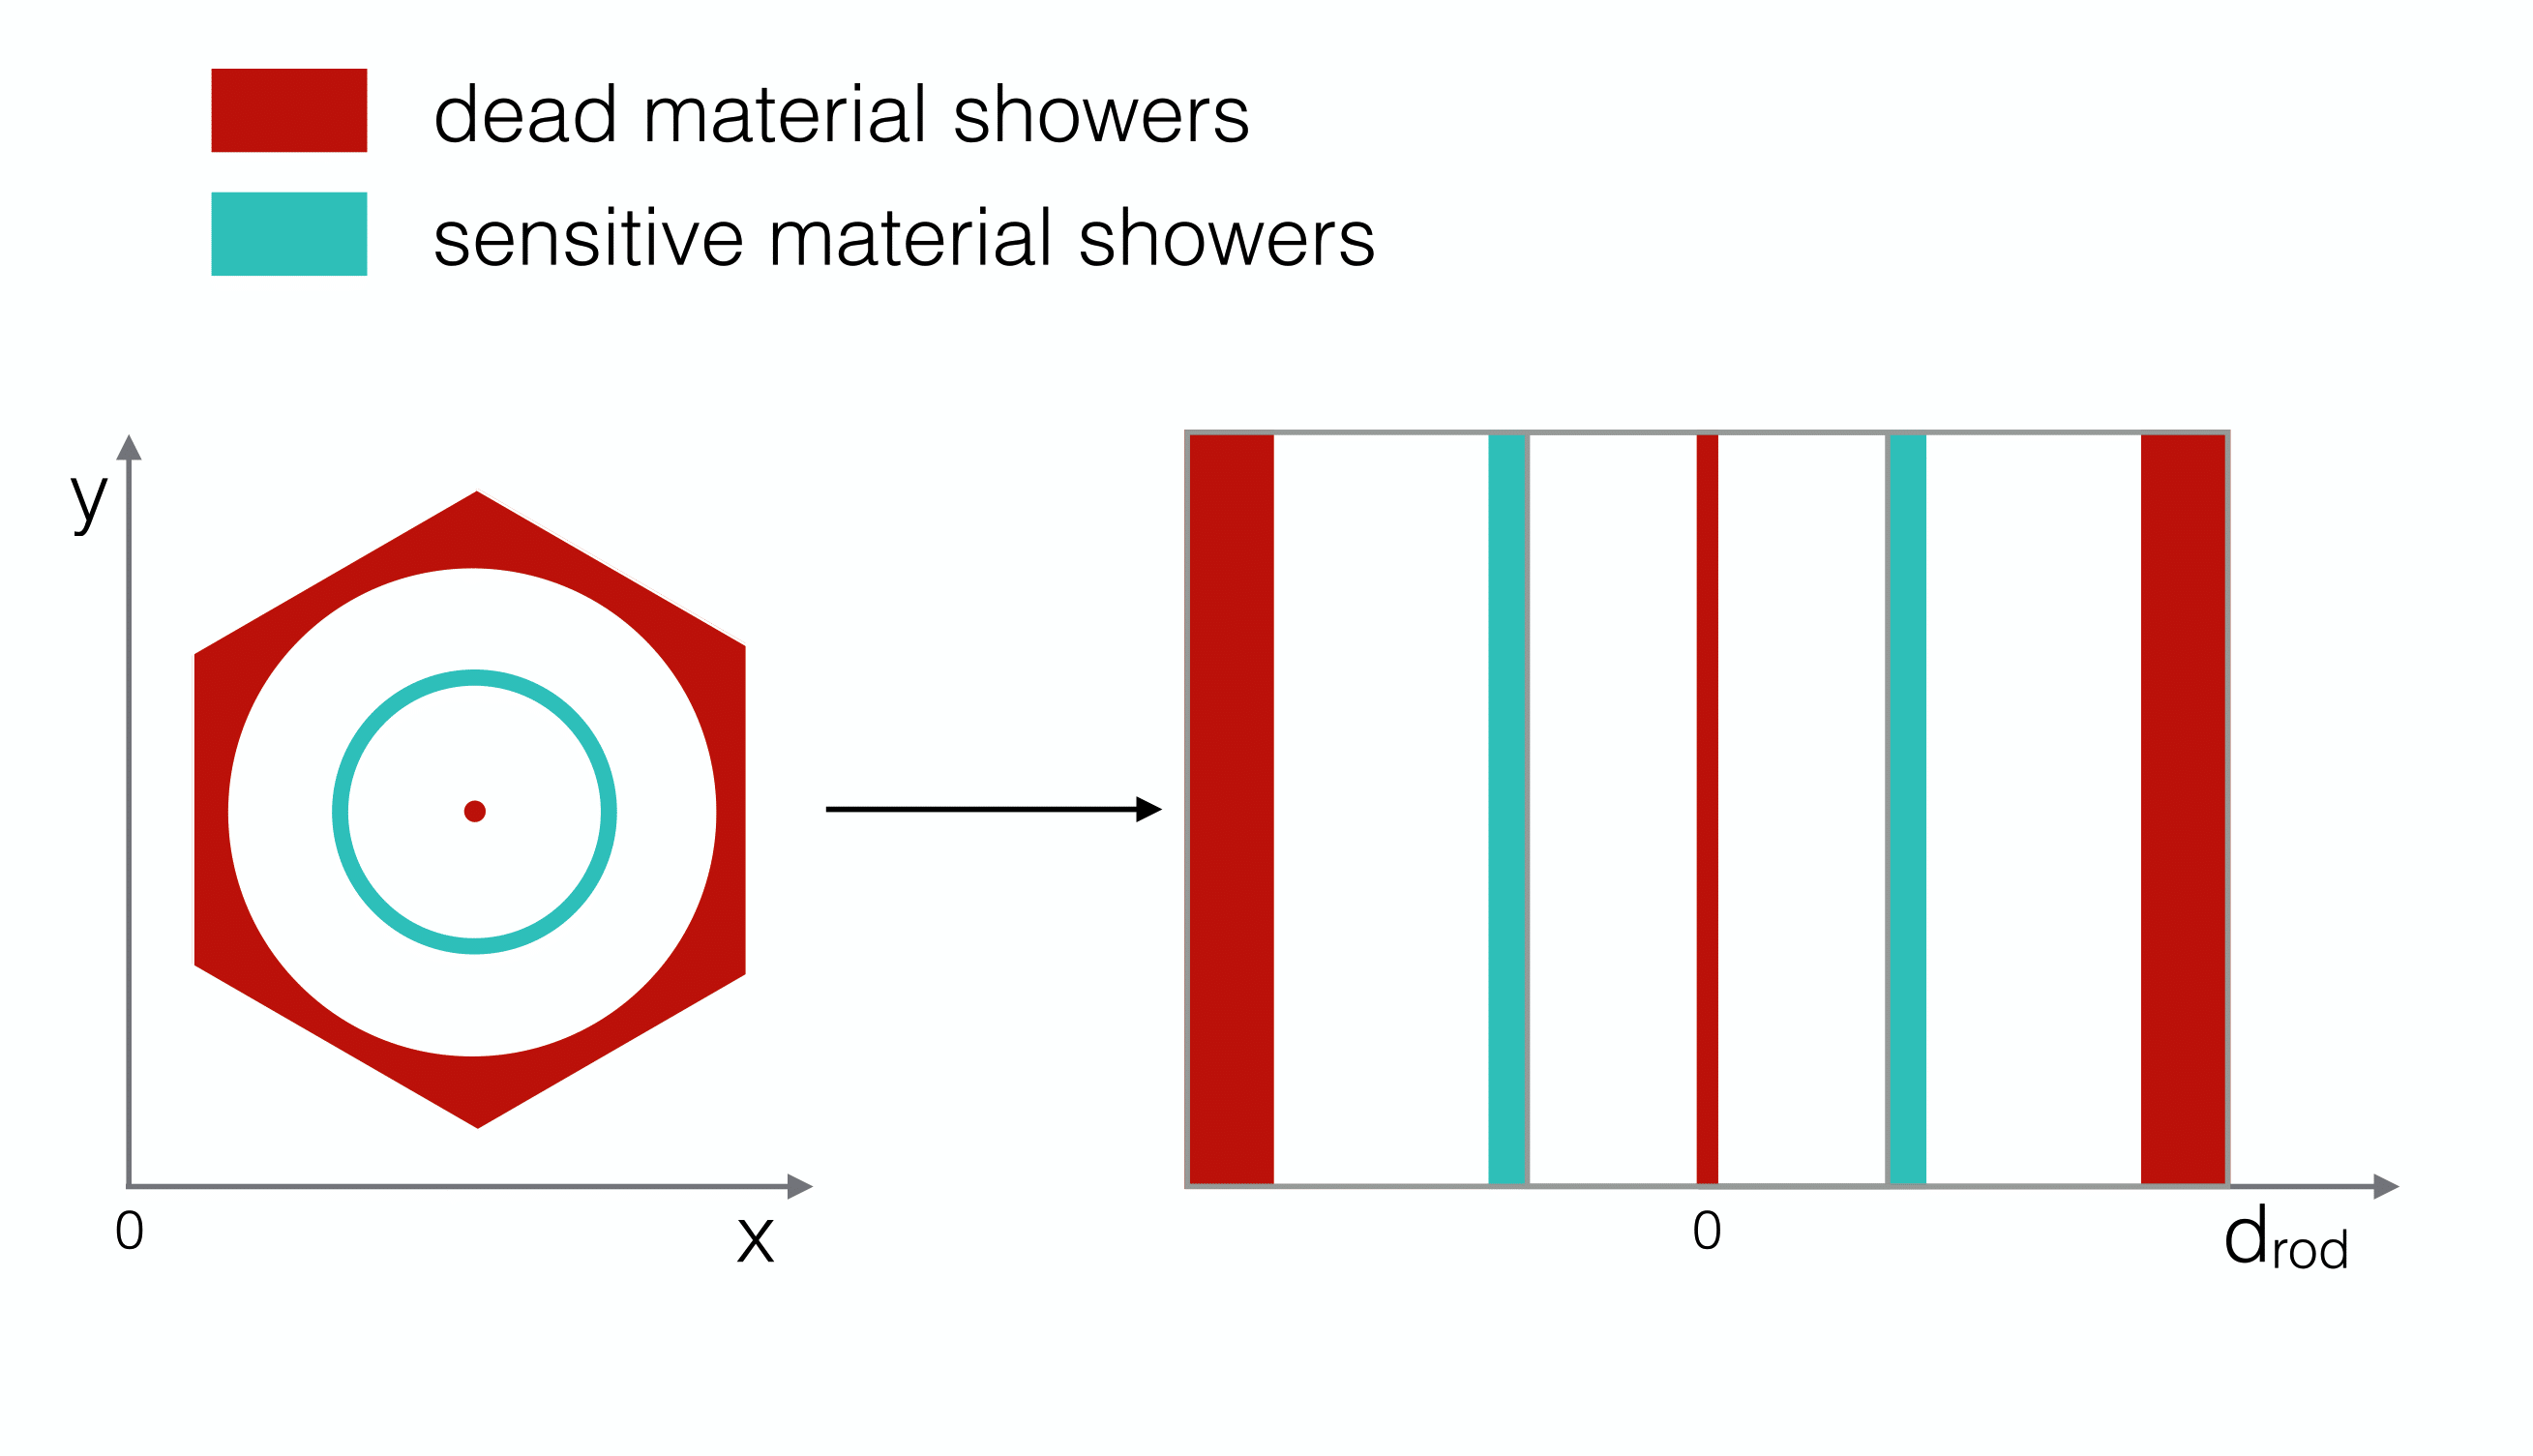
\includegraphics[width=1.0\textwidth]{MC/FirstClassifierData.png}
\caption{Schematic representation of the preselected data for the first classifier in the x-y (left) and distance(right) plane. Electrons, created near the rod center and on the borders of the module have low probability to cross the sensitive material, while those created inside the liquid argon gap are considered as sensitive material showers.}
\label{fig:SchemePresel}}
\end{figure}

\subsubsection{Second classifier}

\begin{figure}[!tbp]
\begin{minipage}[h]{0.49\linewidth}
\center{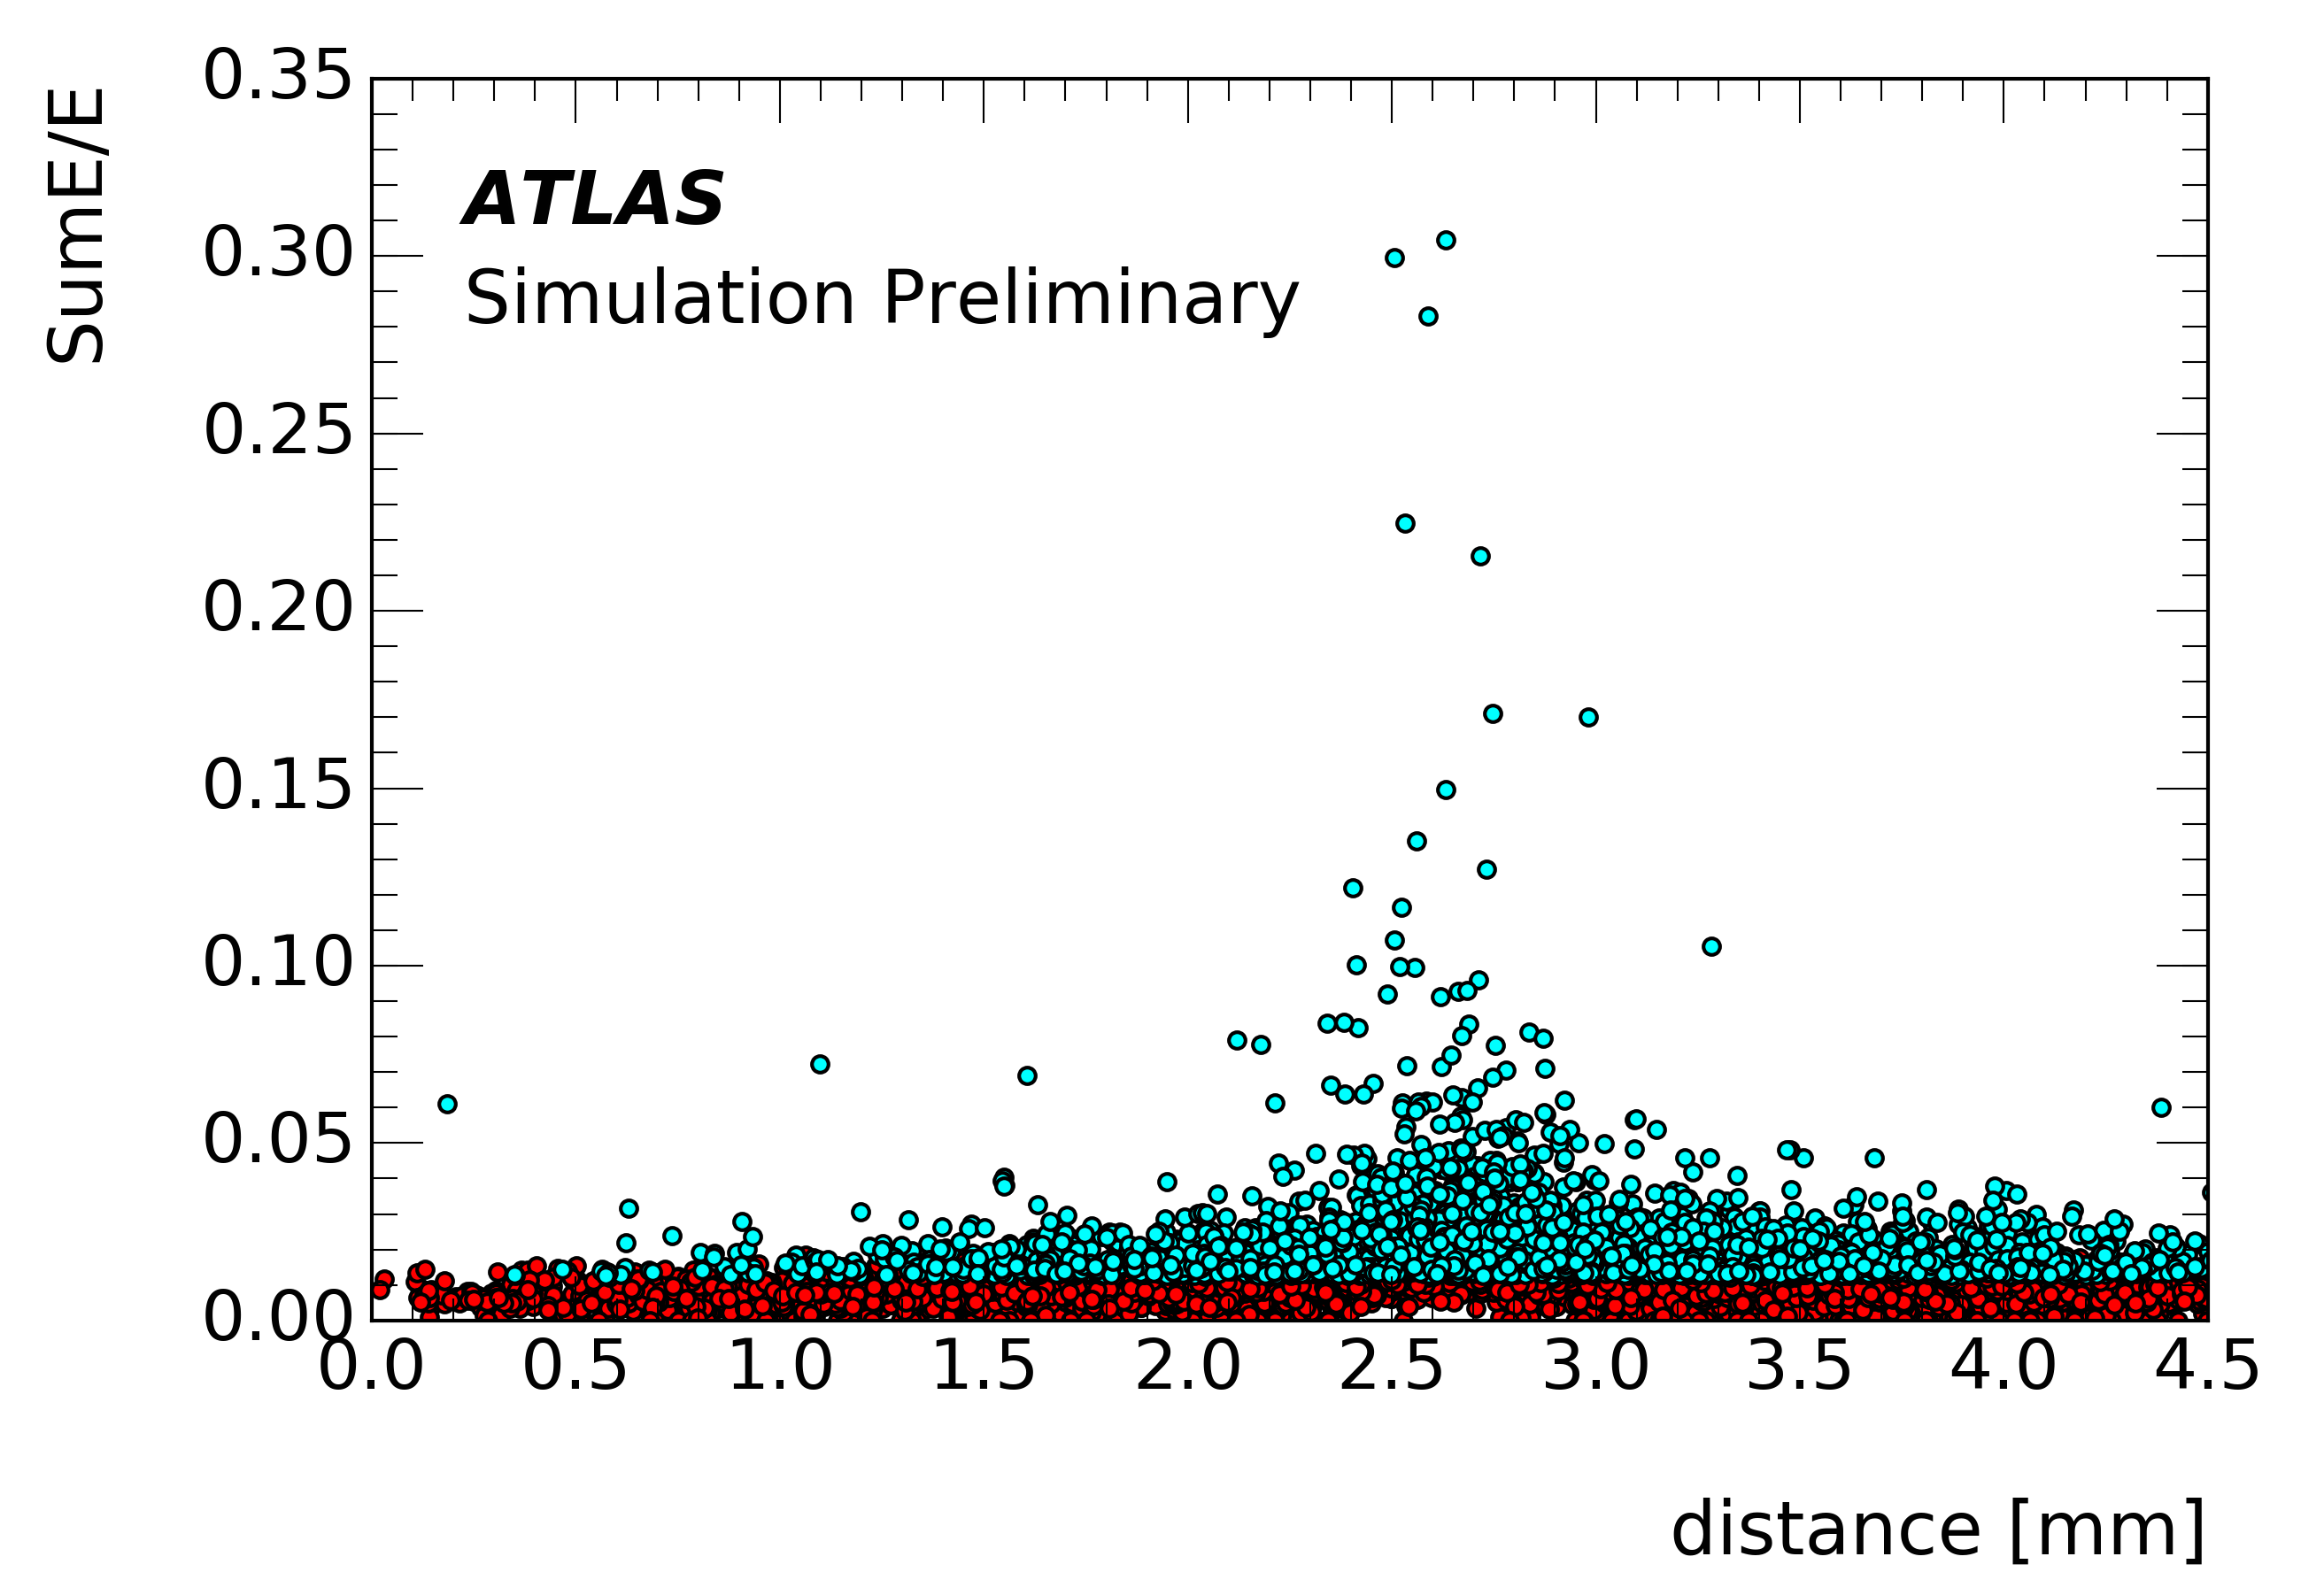
\includegraphics[width=1.\linewidth]{MC/firstClassifier.png} \\ a)}
\end{minipage}
\hfill
\begin{minipage}[h]{0.49\linewidth}
\center{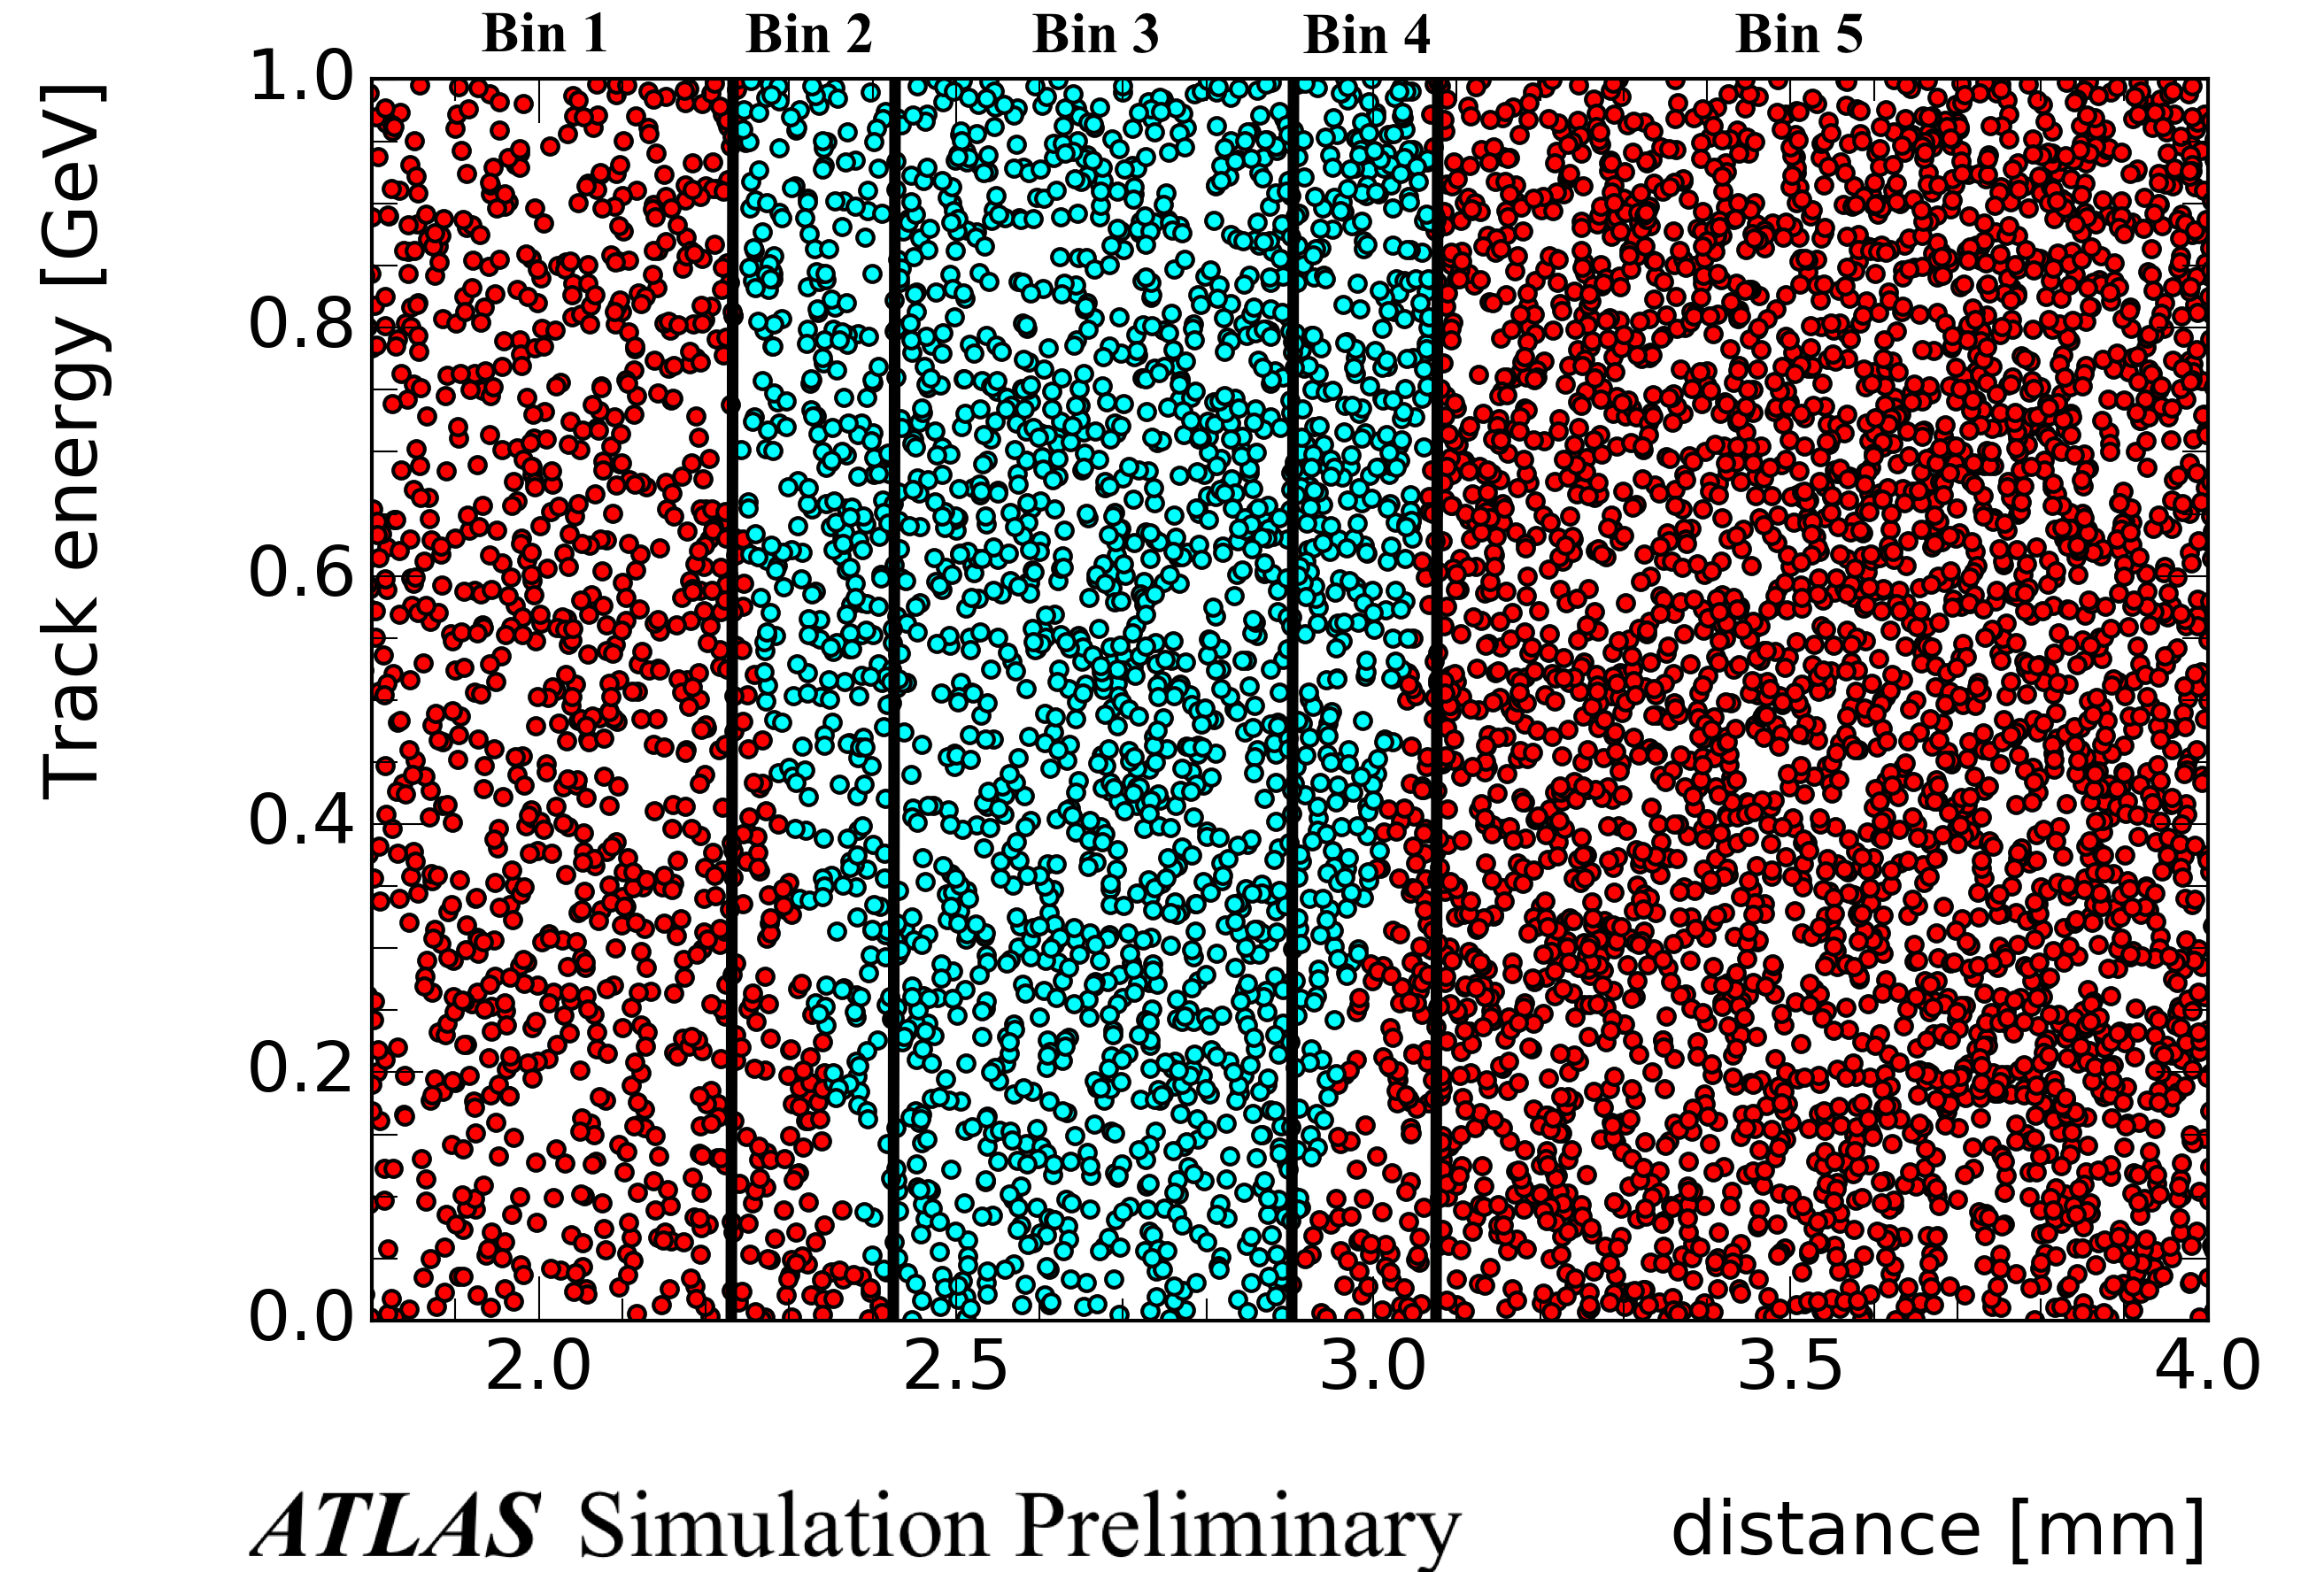
\includegraphics[width=1.\linewidth]{MC/secondClassifier.png} \\ b)}
\end{minipage}
\caption{Results of machine learning algorithm classification for a) first classifier b) second classifier. Cyan dots correspond to sensitive material showers, red to dead material showers. The black lines in Fig. b correspond to the resulting bin positions.}
\label{fig:Class}
\end{figure}

The second classifier uses predictions of the first classifier as input label. 

It reconstructs a best dividing hyperplane between two types of shower using a support vector machines. It uses as input the truth parameters of the electron, e.g. energy of the initial electron and its distance to the closest rod center. Different kernels have been tested and the best predictions have been obtained using RBF kernel (Eq. \ref{eq:RBF}).  Assuming, that $\eta^{momentum} \approx \eta^{position}$ a classification is performed in each $\eta^{distance}$ bin used in the library. 

An example of the classifier output is shown in a Fig. \ref{fig:Class} b). The obtained gap positions are wider, than the original ones, as it is expected from the model.  Variation of the obtained parameters have been found small, so the mean of the parameters has been as an input for the binning.  

\subsection{Interpretation of results}

Since full new regeneration of libraries and the validation of reconstructed variables is time-consuming procedure, a Monte Carlo method has been developed for a cross-check of the classifiers and its interpretation. It uses pseudorapidity $\eta^{position}$, energy of electron and distance to the closest rod center from the data as a reference for the random generator. This simulation allows to compare the shower energies and shower energies divided by  the energy of the initial electron (SumE/E) distributions with the distributions coming from the full simulation, which are considered as a reference.

The resulting hyperplane from second classifier can be translated to the bin positions in the different ways. Several interpretations of the bin positions have been tested and the best one is shown in Fig.~\ref{fig:Class} b) with black lines. The best SumE/E agreemen have been achieved using three bins in liquid argon position instead of the only one. The central bin, according to the classifier, contains just sensitive material showers events, while the other two there is a mixture of dead and sensitive material showers. The obtained positions of the liquid argon bins are wider, than the nominal ones for both FCAL1 and FCAL2.

Comparison of SumE/E distributions using toy MC on old libraries (Fig. ~\ref{fig:Interpret} a) and the libraries with the new binning (Fig. ~\ref{fig:Interpret} b) has shown, that we could expect a better performance on the reconstructed values for the new binning.

\begin{figure}[!tbp]
\begin{minipage}[h]{0.49\linewidth}
\center{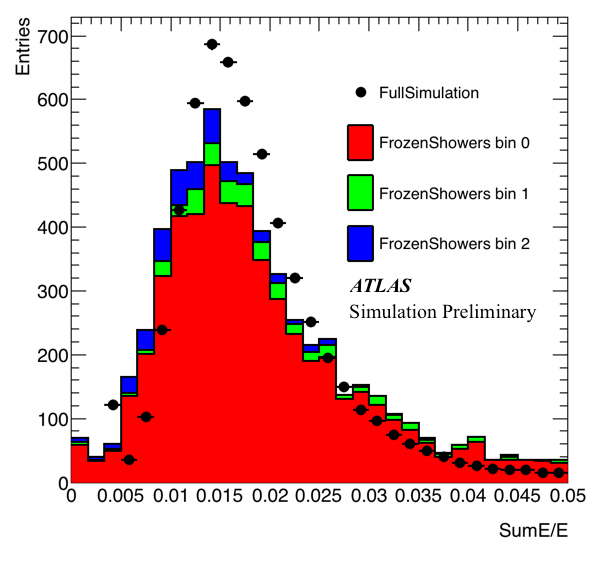
\includegraphics[width=1.\linewidth]{MC/oldSumE.png} \\ a)}
\end{minipage}
\hfill
\begin{minipage}[h]{0.49\linewidth}
\center{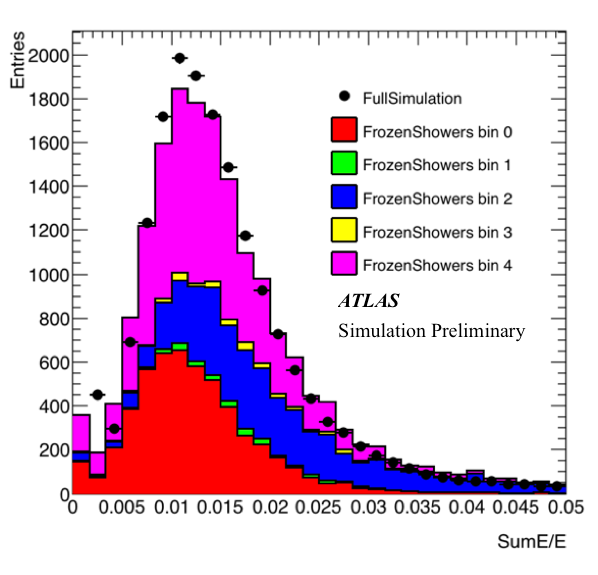
\includegraphics[width=1.\linewidth]{MC/newSumE.png} \\ b)}
\end{minipage}
\caption{Comparison of the distributions of shower energy divided by  the energy of the initial electron between full simulation and toy MC using libraries for liquid argon gap bins and 2 closest to them bins for a) old "tuned" libraries with 1 liquid argon gap bin  b) new libraries using 3 liquid argon gap bins. There are still remaining differences between full simulation and toy MC, but the new machine learning binning gives a better agreement with full simulation.}
\label{fig:Interpret}
\end{figure}


\subsection{Reconstructed electron energy}

Since the resolution of the single electrons can have a significant difference, the energies of reconstructed electrons are validated before the mass validation of the different groups. Measurement of the shift in the mean energy between full and fast simulation allows to correct the scale for frozen showers.

Validation is performed for the following electron energies: 100 GeV, 200 GeV, 500 GeV and 1000 GeV and within the $\eta$ directions that are corresponding to the 12 $\eta$ bins of the library. The resolution is calculated as RMS of all reconstructed energies for the certain energy and $\eta$. The results of the electron resolution validation for the new machine learning based binning and old "tuned" libraries is shown in Fig. \ref{fig:Reso}. The new methods gives a better of comparable resolution agreement than an old libraries. However, there are 2 bins, there new method resolution is significantly worse, than old one (3.5 and 4.3). This means, that this method still needs to be improved. The possible ways of its improvement are discussed in Sec. \ref{sec:FSImpr}.

In a meanwhile it was decided to use a combination of the new and old libraries. The mean shift is corrected as described in Sec. \ref{sec:LibTuning} and showed in Fig. \ref{fig:Mean}. The remaining differences between full and fast simulation are considered negligible.


\begin{figure}[!tbp]
\begin{minipage}[h]{0.32\linewidth}
\center{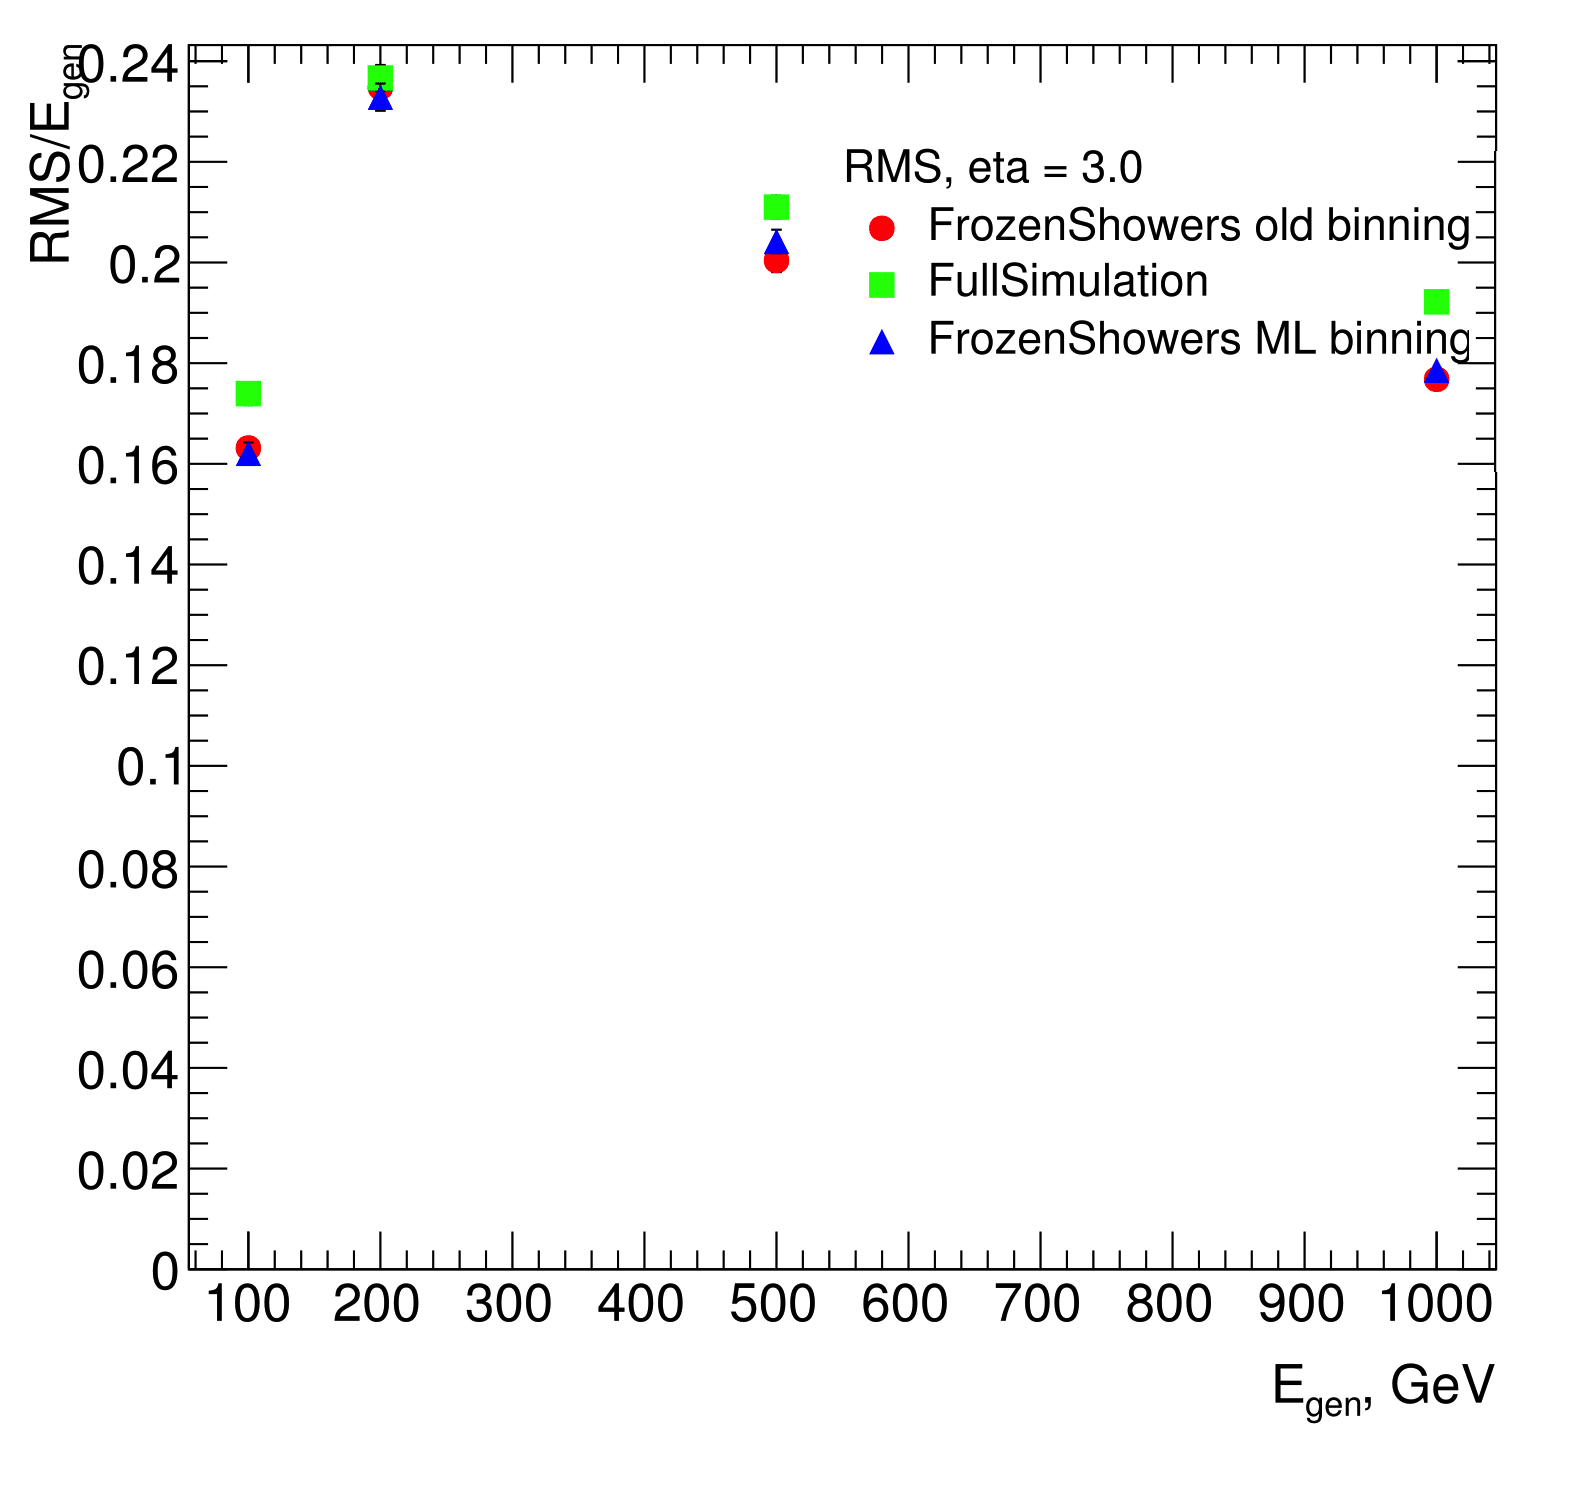
\includegraphics[width=1.\linewidth]{MC/RMS/RMS-12.png} }
\end{minipage}
\hfill
\begin{minipage}[h]{0.32\linewidth}
\center{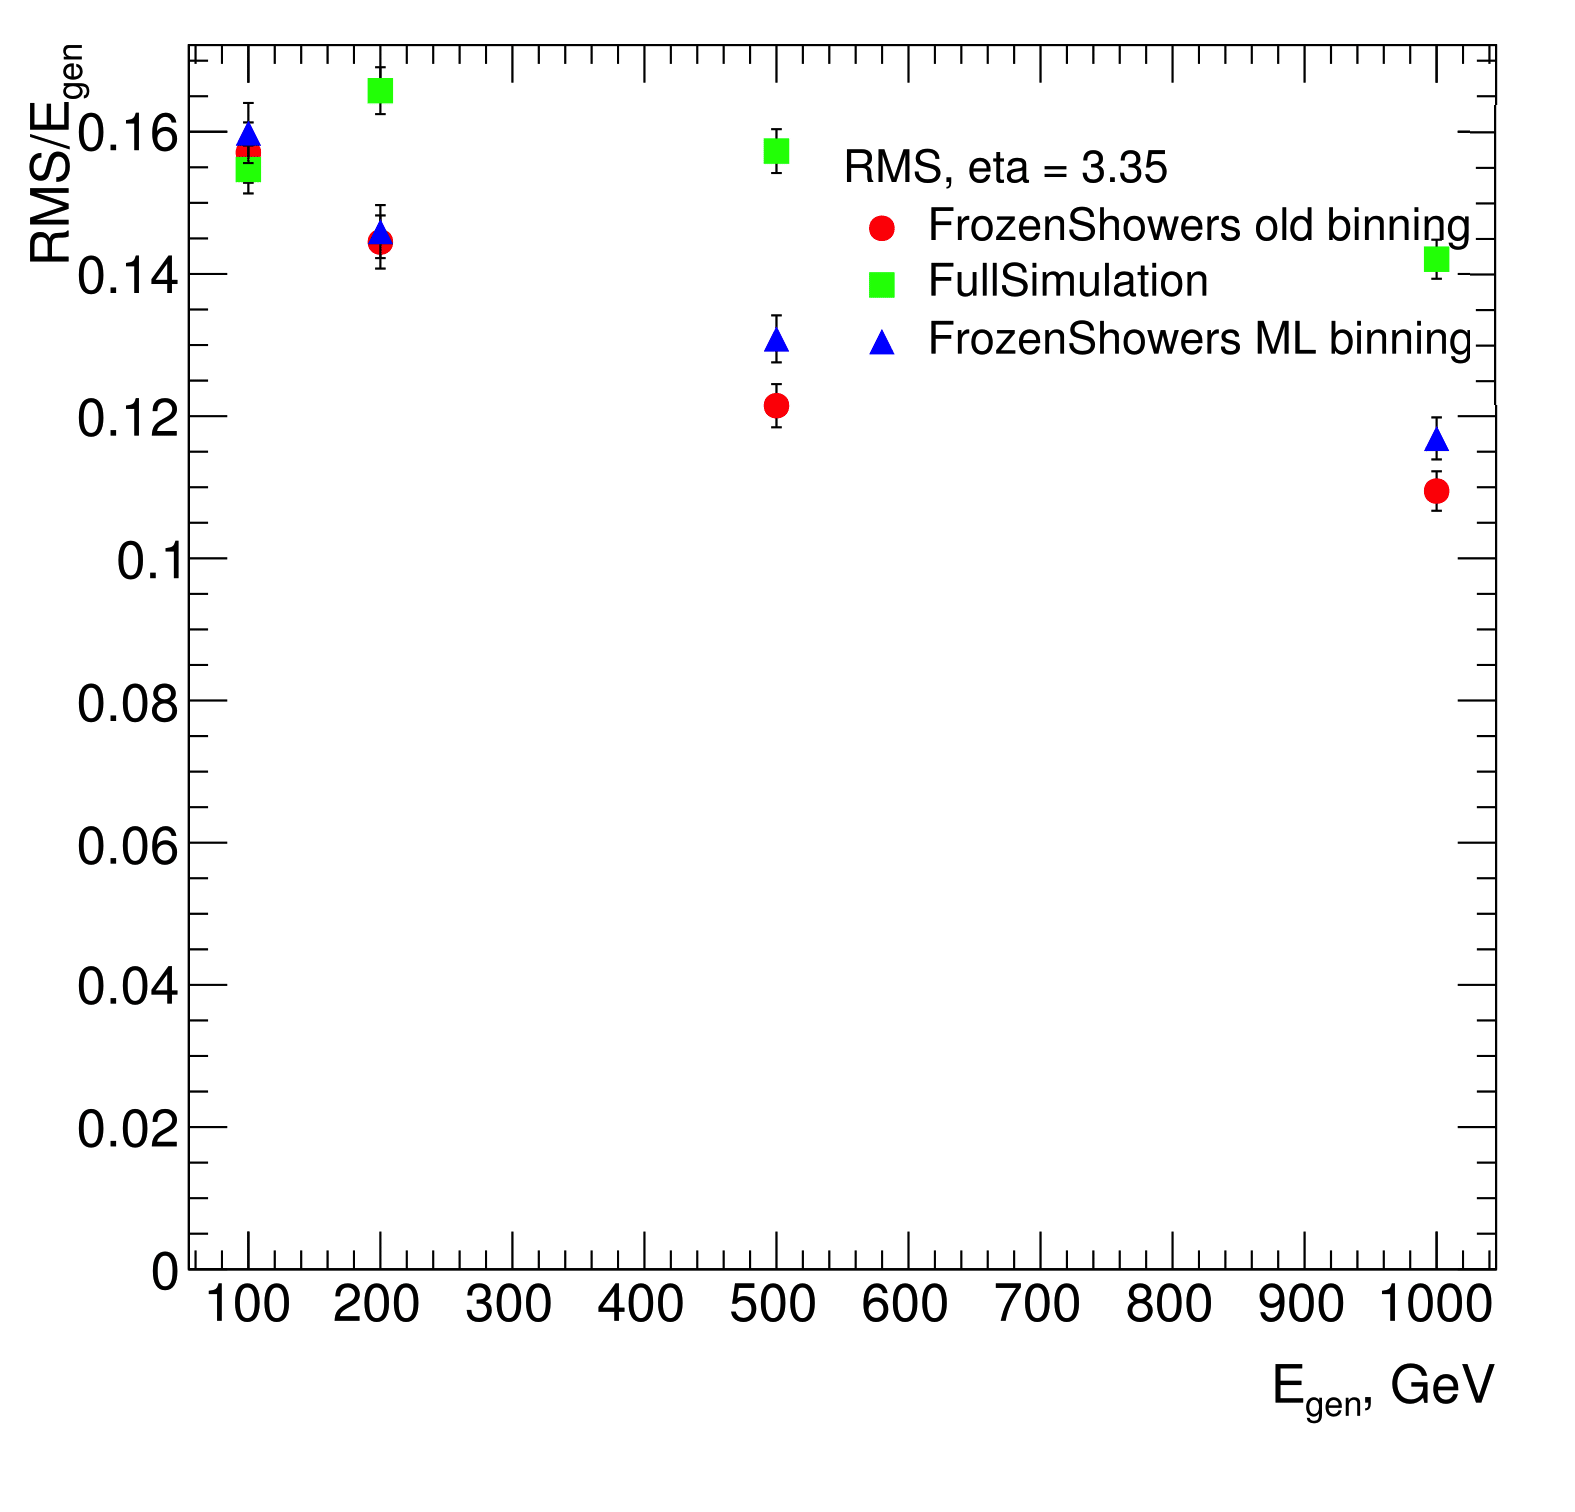
\includegraphics[width=1.\linewidth]{MC/RMS/RMS-11.png} }
\end{minipage}
\hfill
\begin{minipage}[h]{0.32\linewidth}
\center{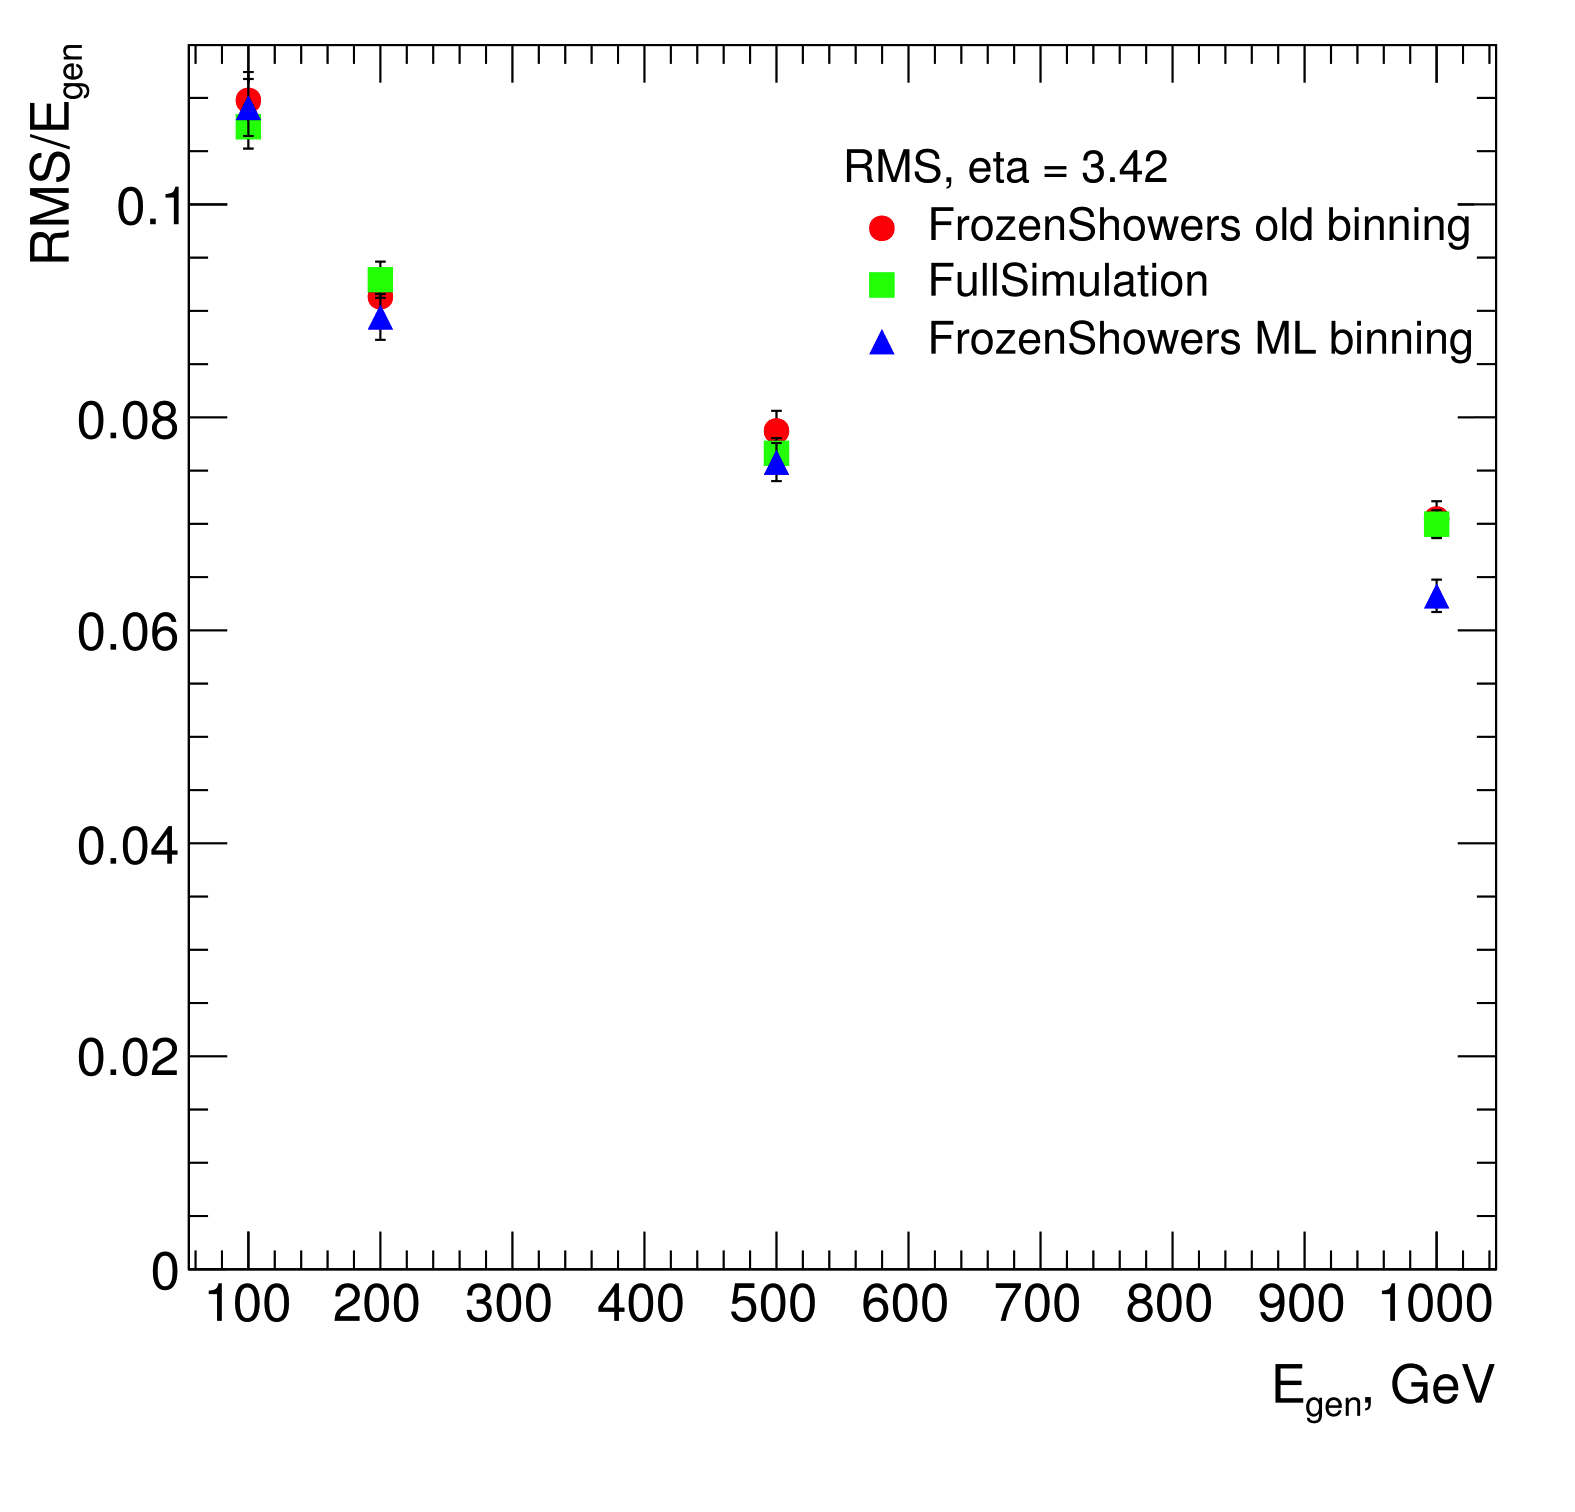
\includegraphics[width=1.\linewidth]{MC/RMS/RMS-10.png}  }
\end{minipage}
\vfill
\begin{minipage}[h]{0.32\linewidth}
\center{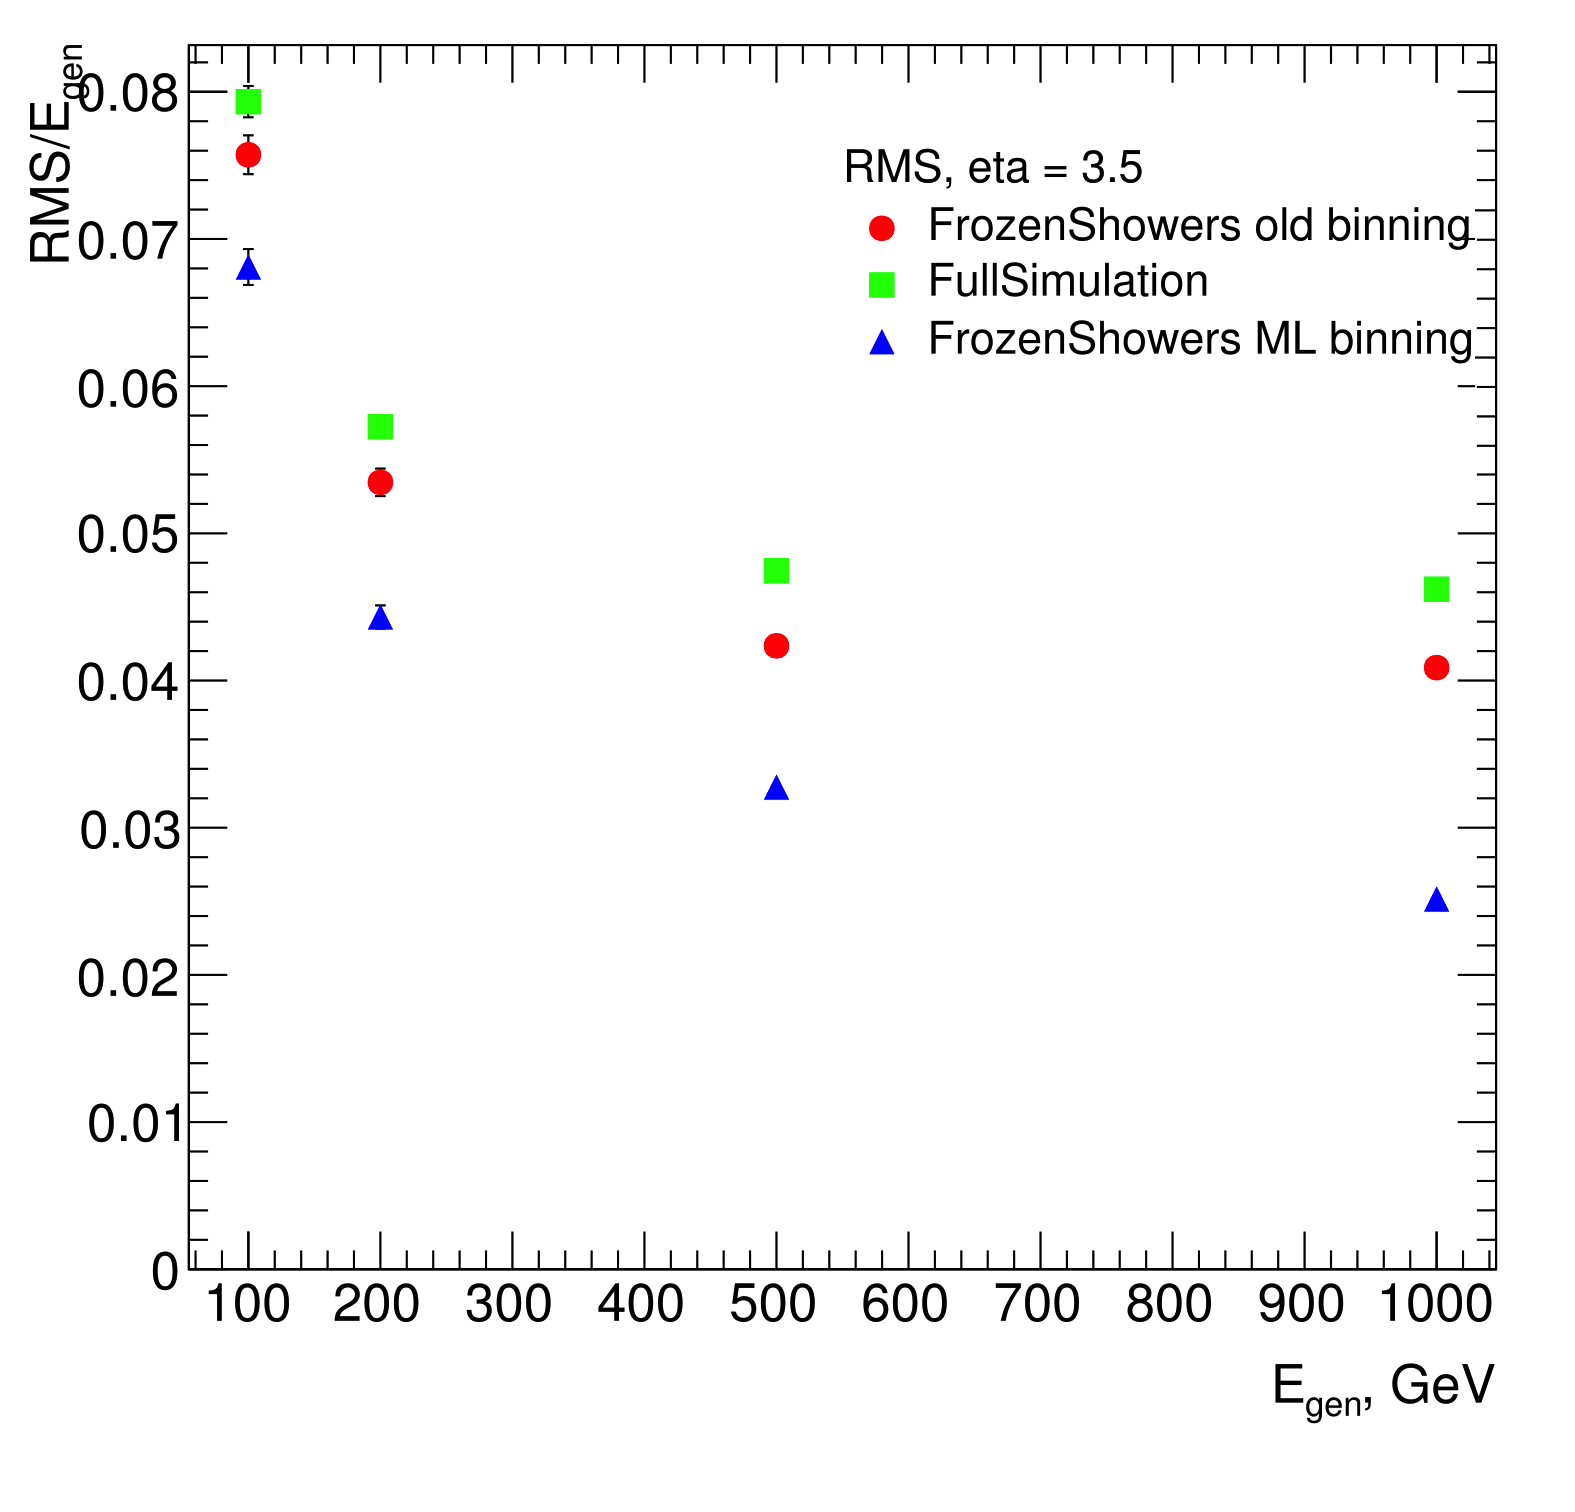
\includegraphics[width=1.\linewidth]{MC/RMS/RMS-09.png}  }
\end{minipage}
\hfill
\begin{minipage}[h]{0.32\linewidth}
\center{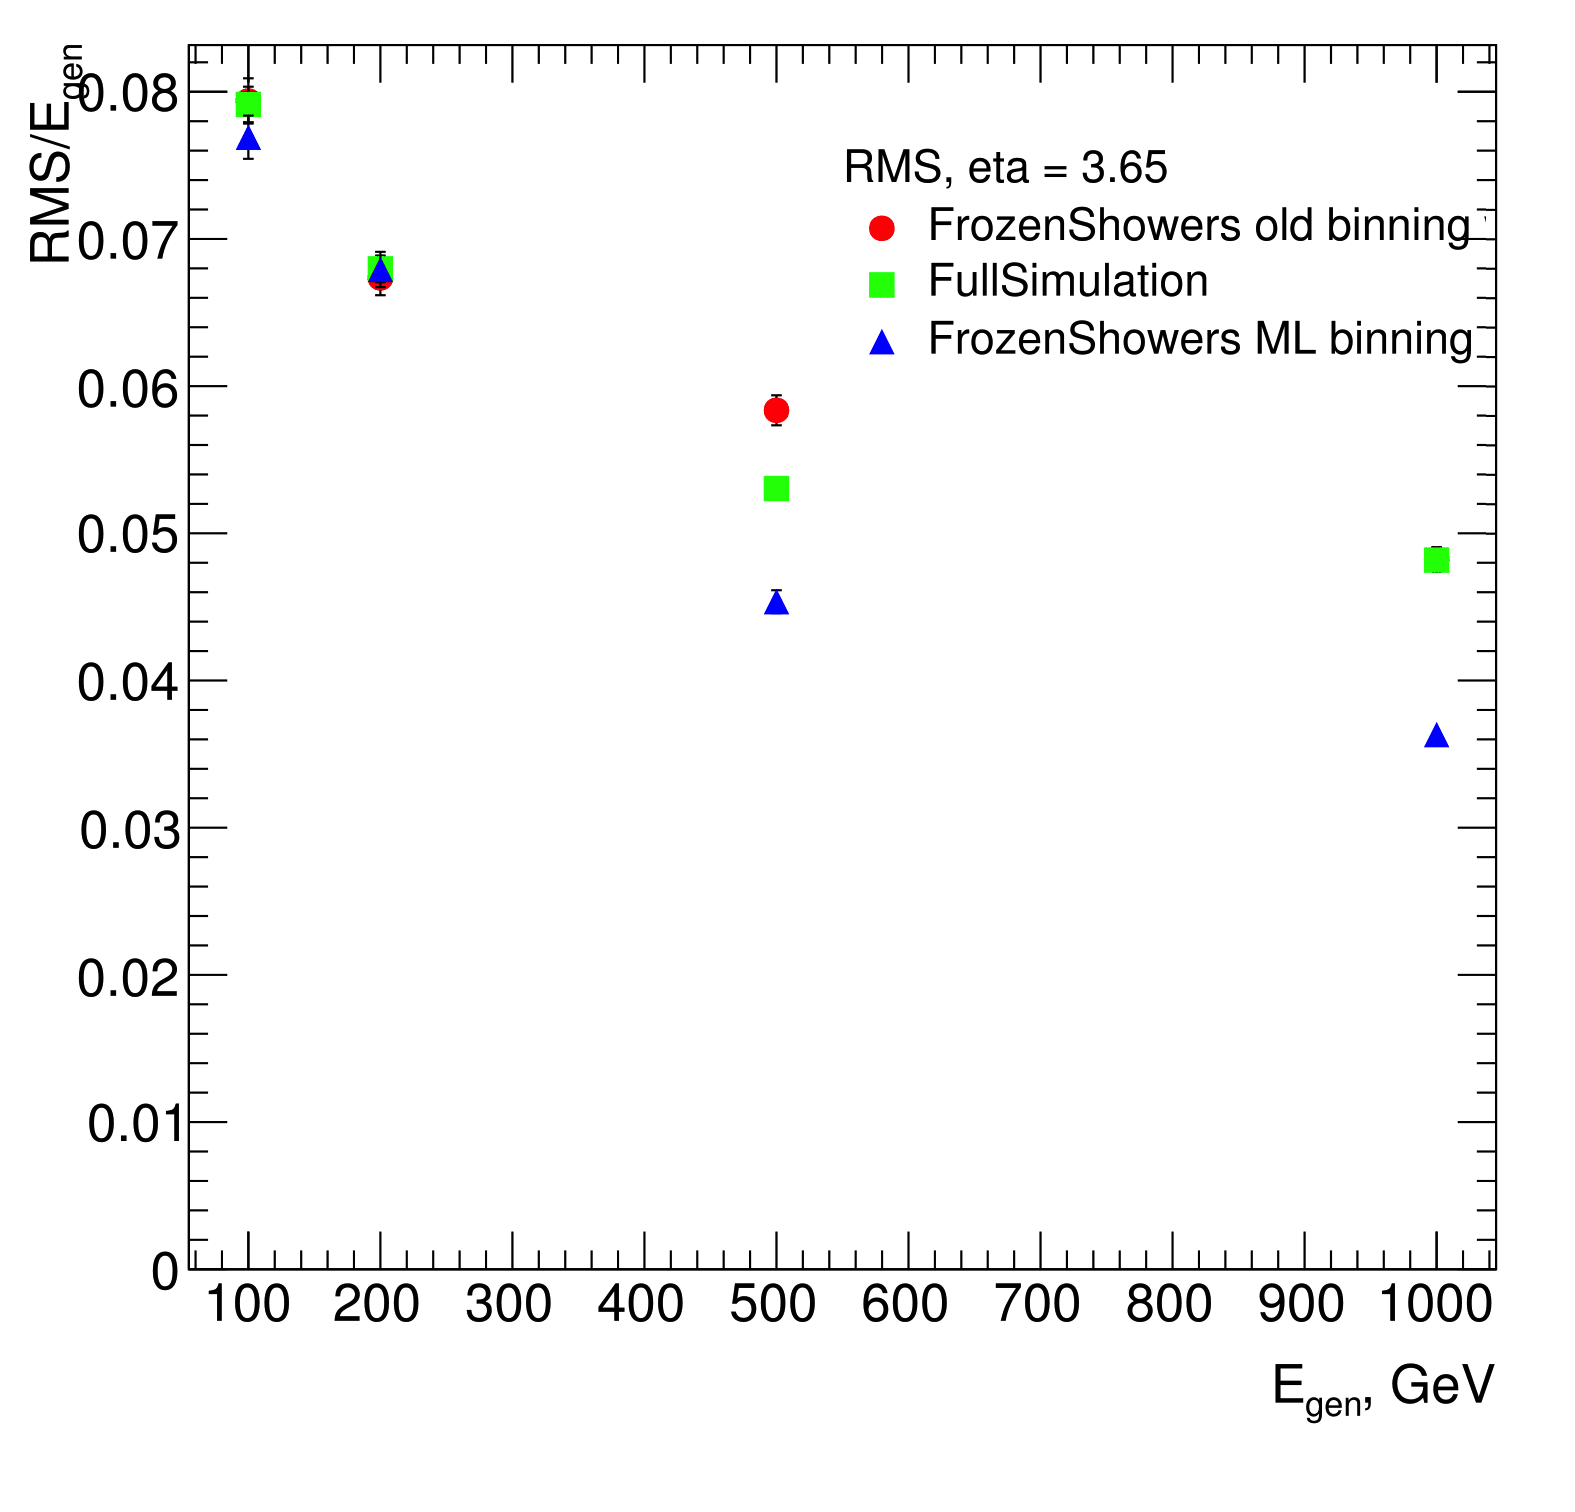
\includegraphics[width=1.\linewidth]{MC/RMS/RMS-08.png} }
\end{minipage}
\hfill
\begin{minipage}[h]{0.32\linewidth}
\center{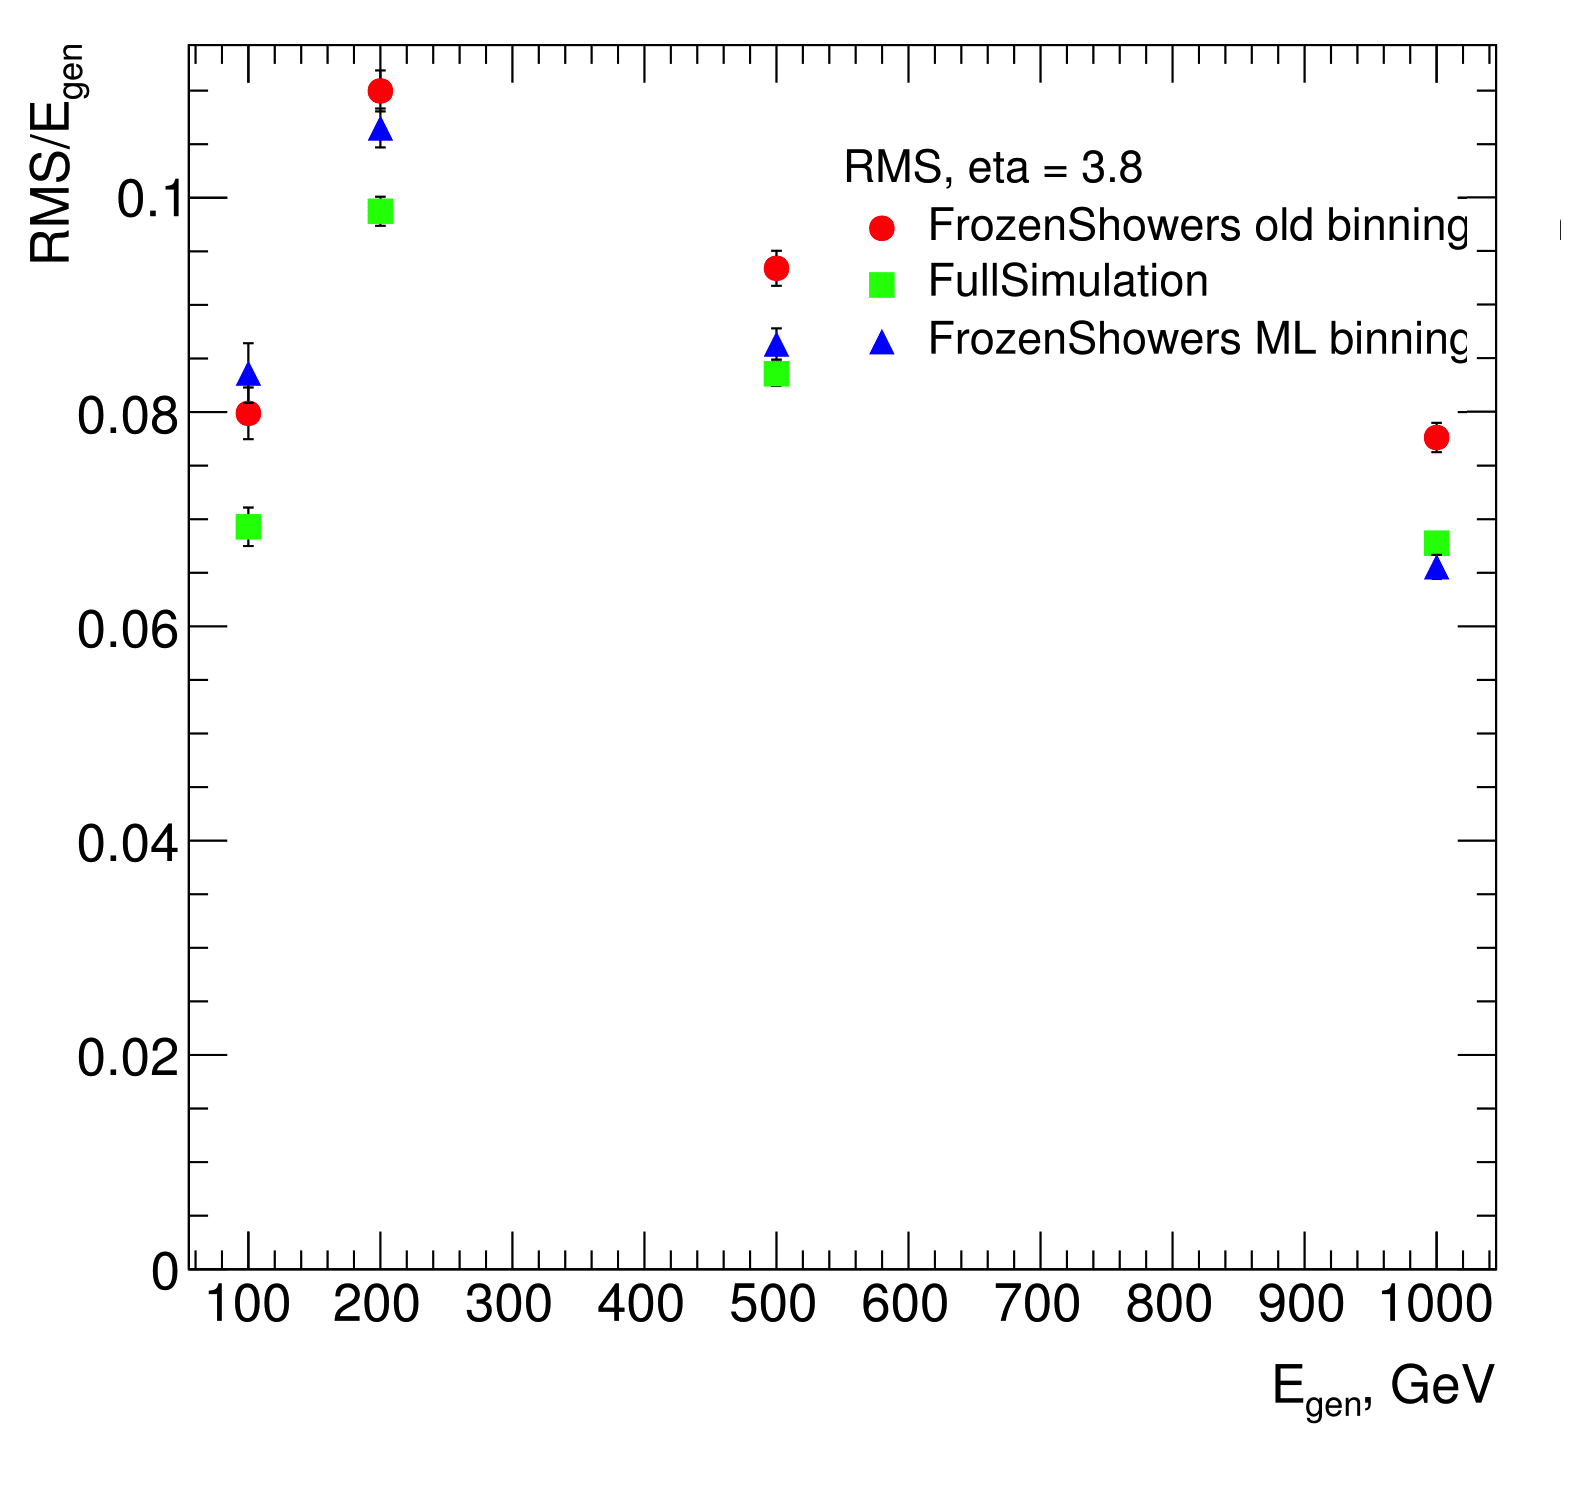
\includegraphics[width=1.\linewidth]{MC/RMS/RMS-07.png}  }
\end{minipage}
\vfill
\begin{minipage}[h]{0.32\linewidth}
\center{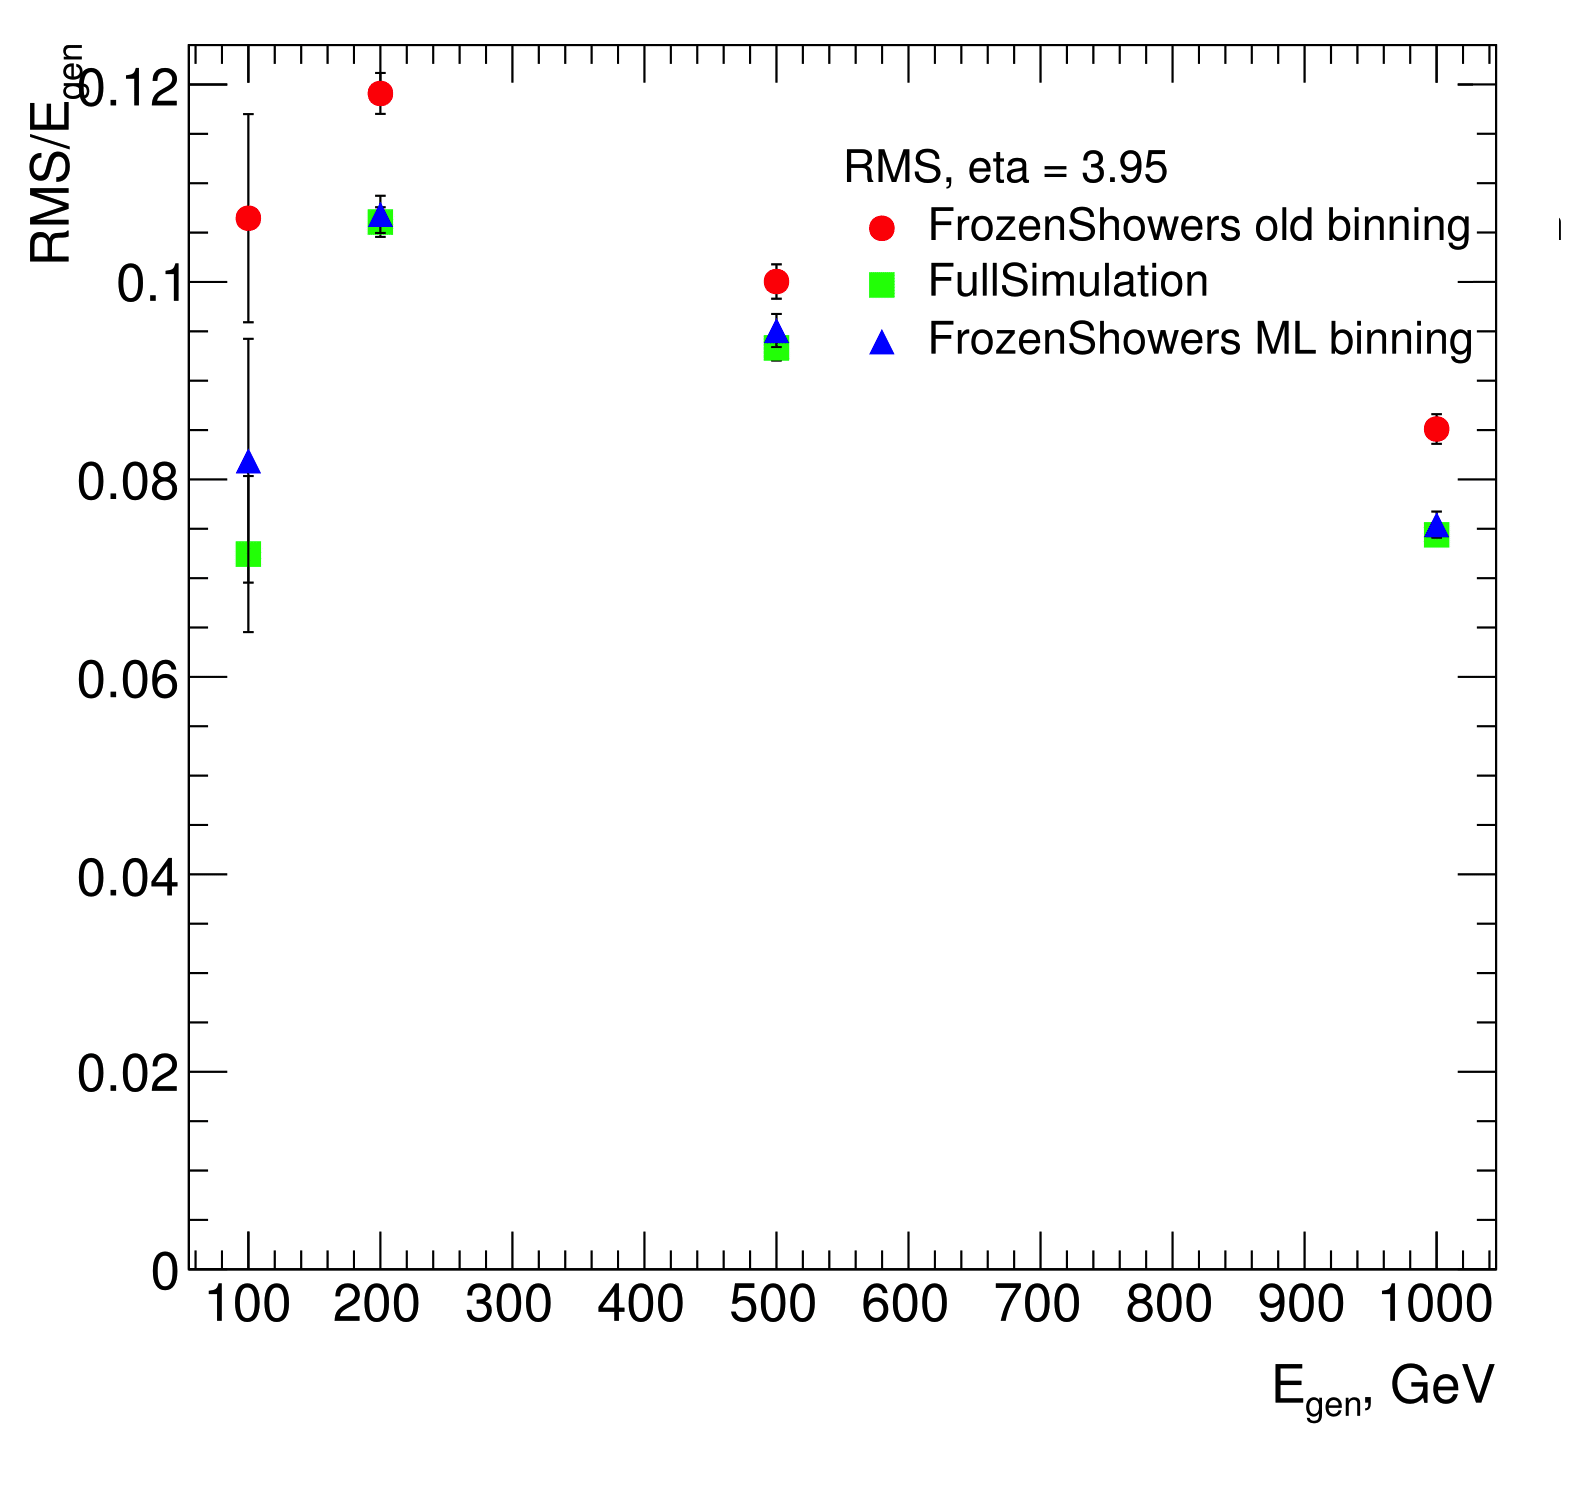
\includegraphics[width=1.\linewidth]{MC/RMS/RMS-06.png}  }
\end{minipage}
\hfill
\begin{minipage}[h]{0.32\linewidth}
\center{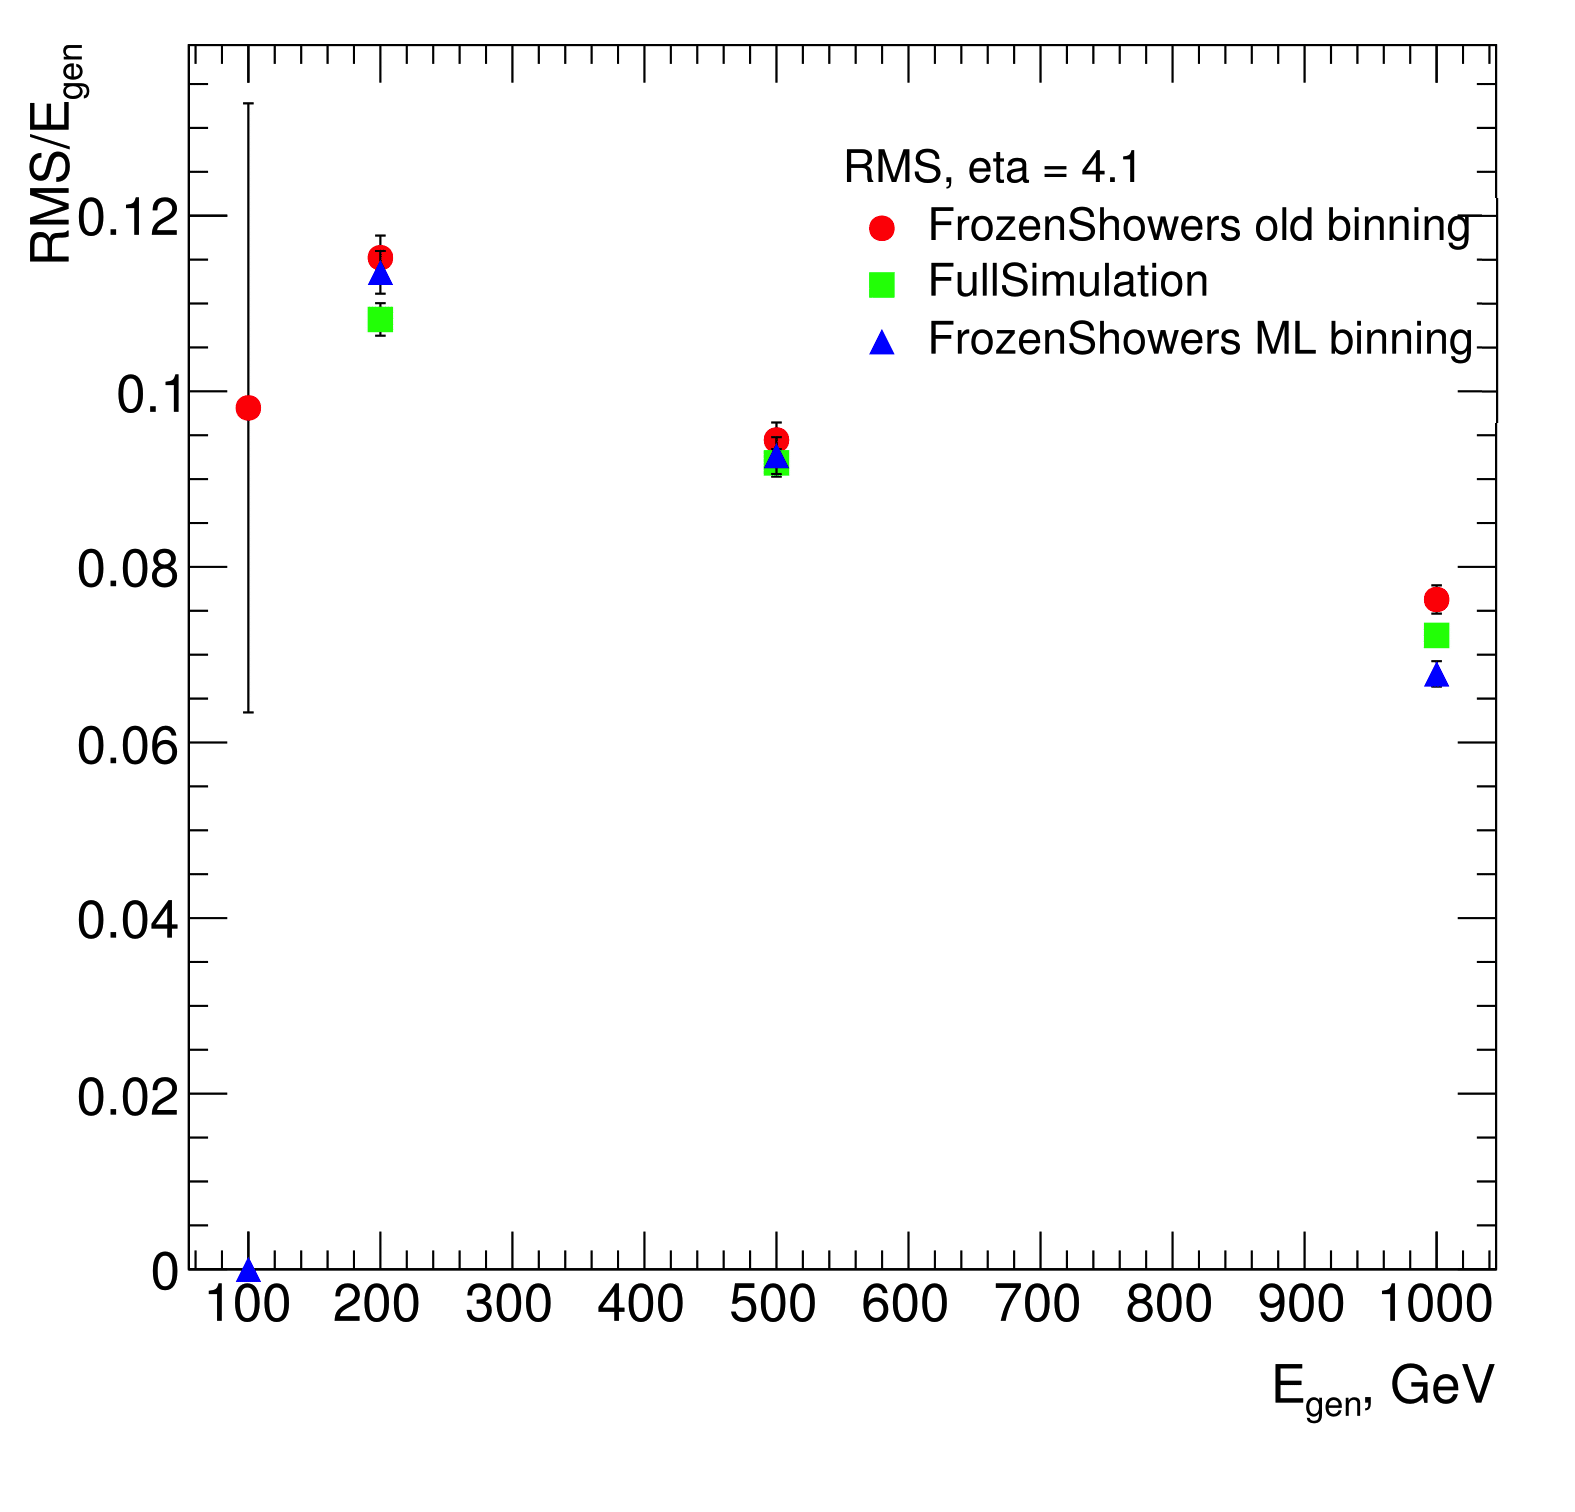
\includegraphics[width=1.\linewidth]{MC/RMS/RMS-05.png}  }
\end{minipage}
\hfill
\begin{minipage}[h]{0.32\linewidth}
\center{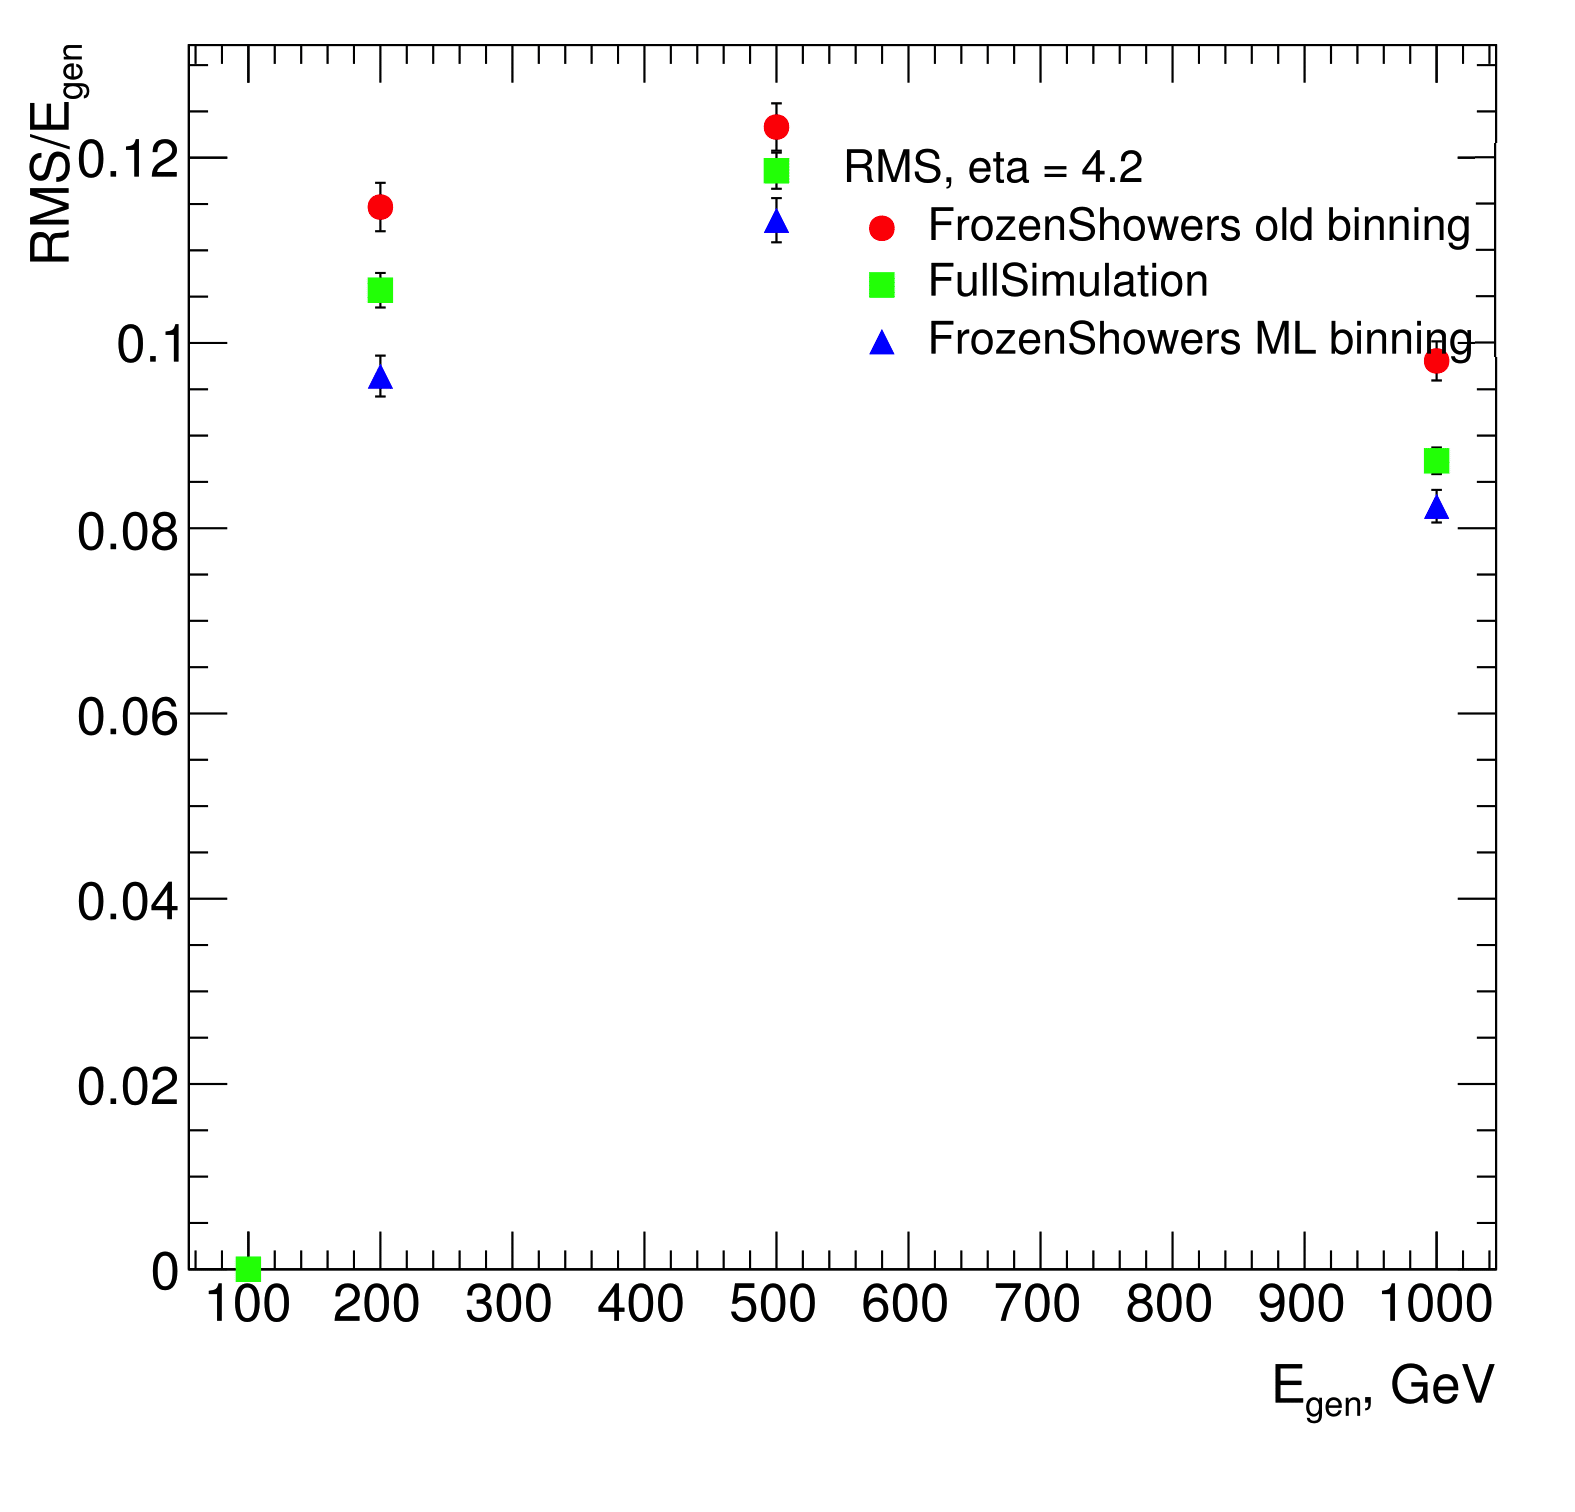
\includegraphics[width=1.\linewidth]{MC/RMS/RMS-04.png}  }
\end{minipage}
\vfill
\begin{minipage}[h]{0.32\linewidth}
\center{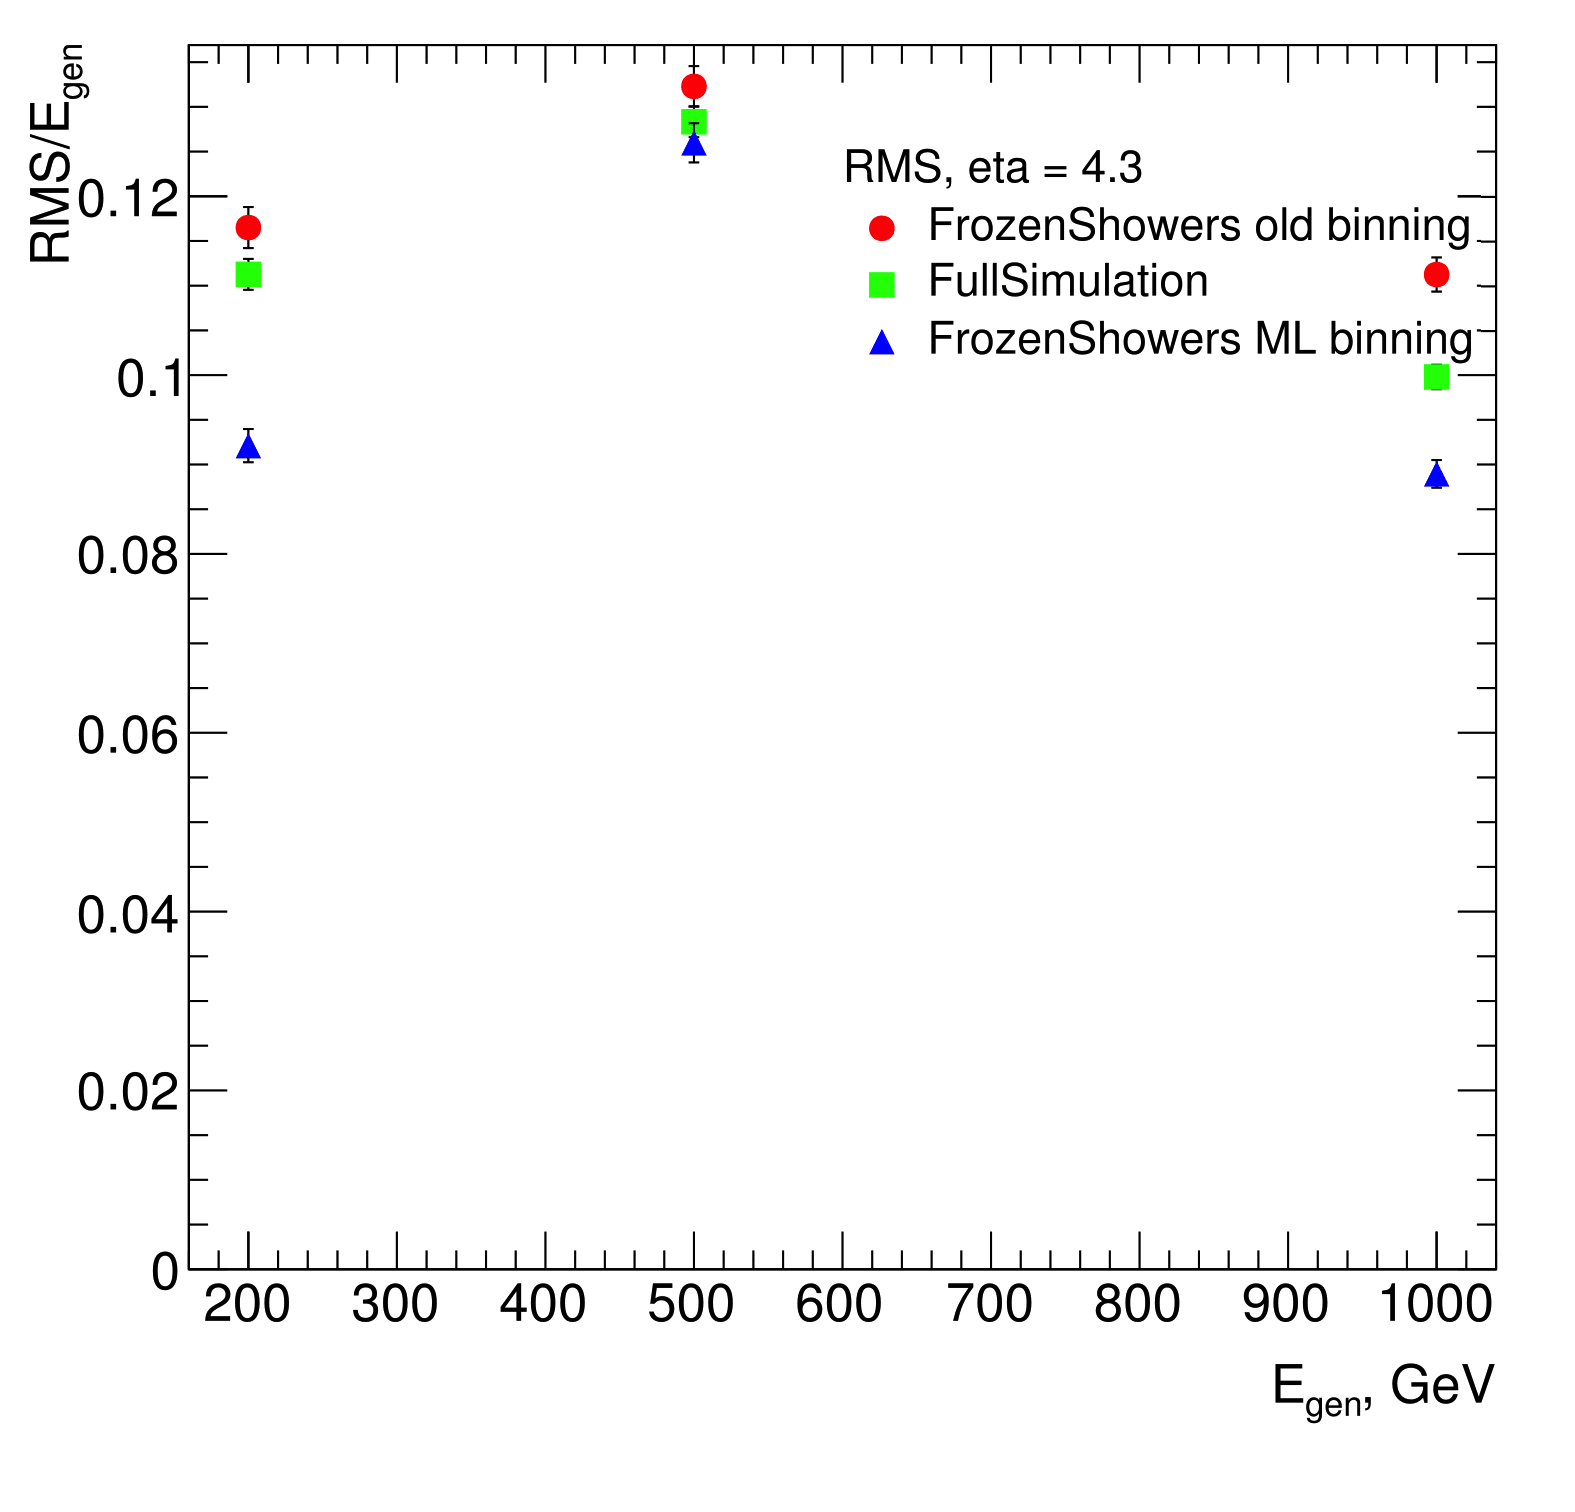
\includegraphics[width=1.\linewidth]{MC/RMS/RMS-03.png}  }
\end{minipage}
\hfill
\begin{minipage}[h]{0.32\linewidth}
\center{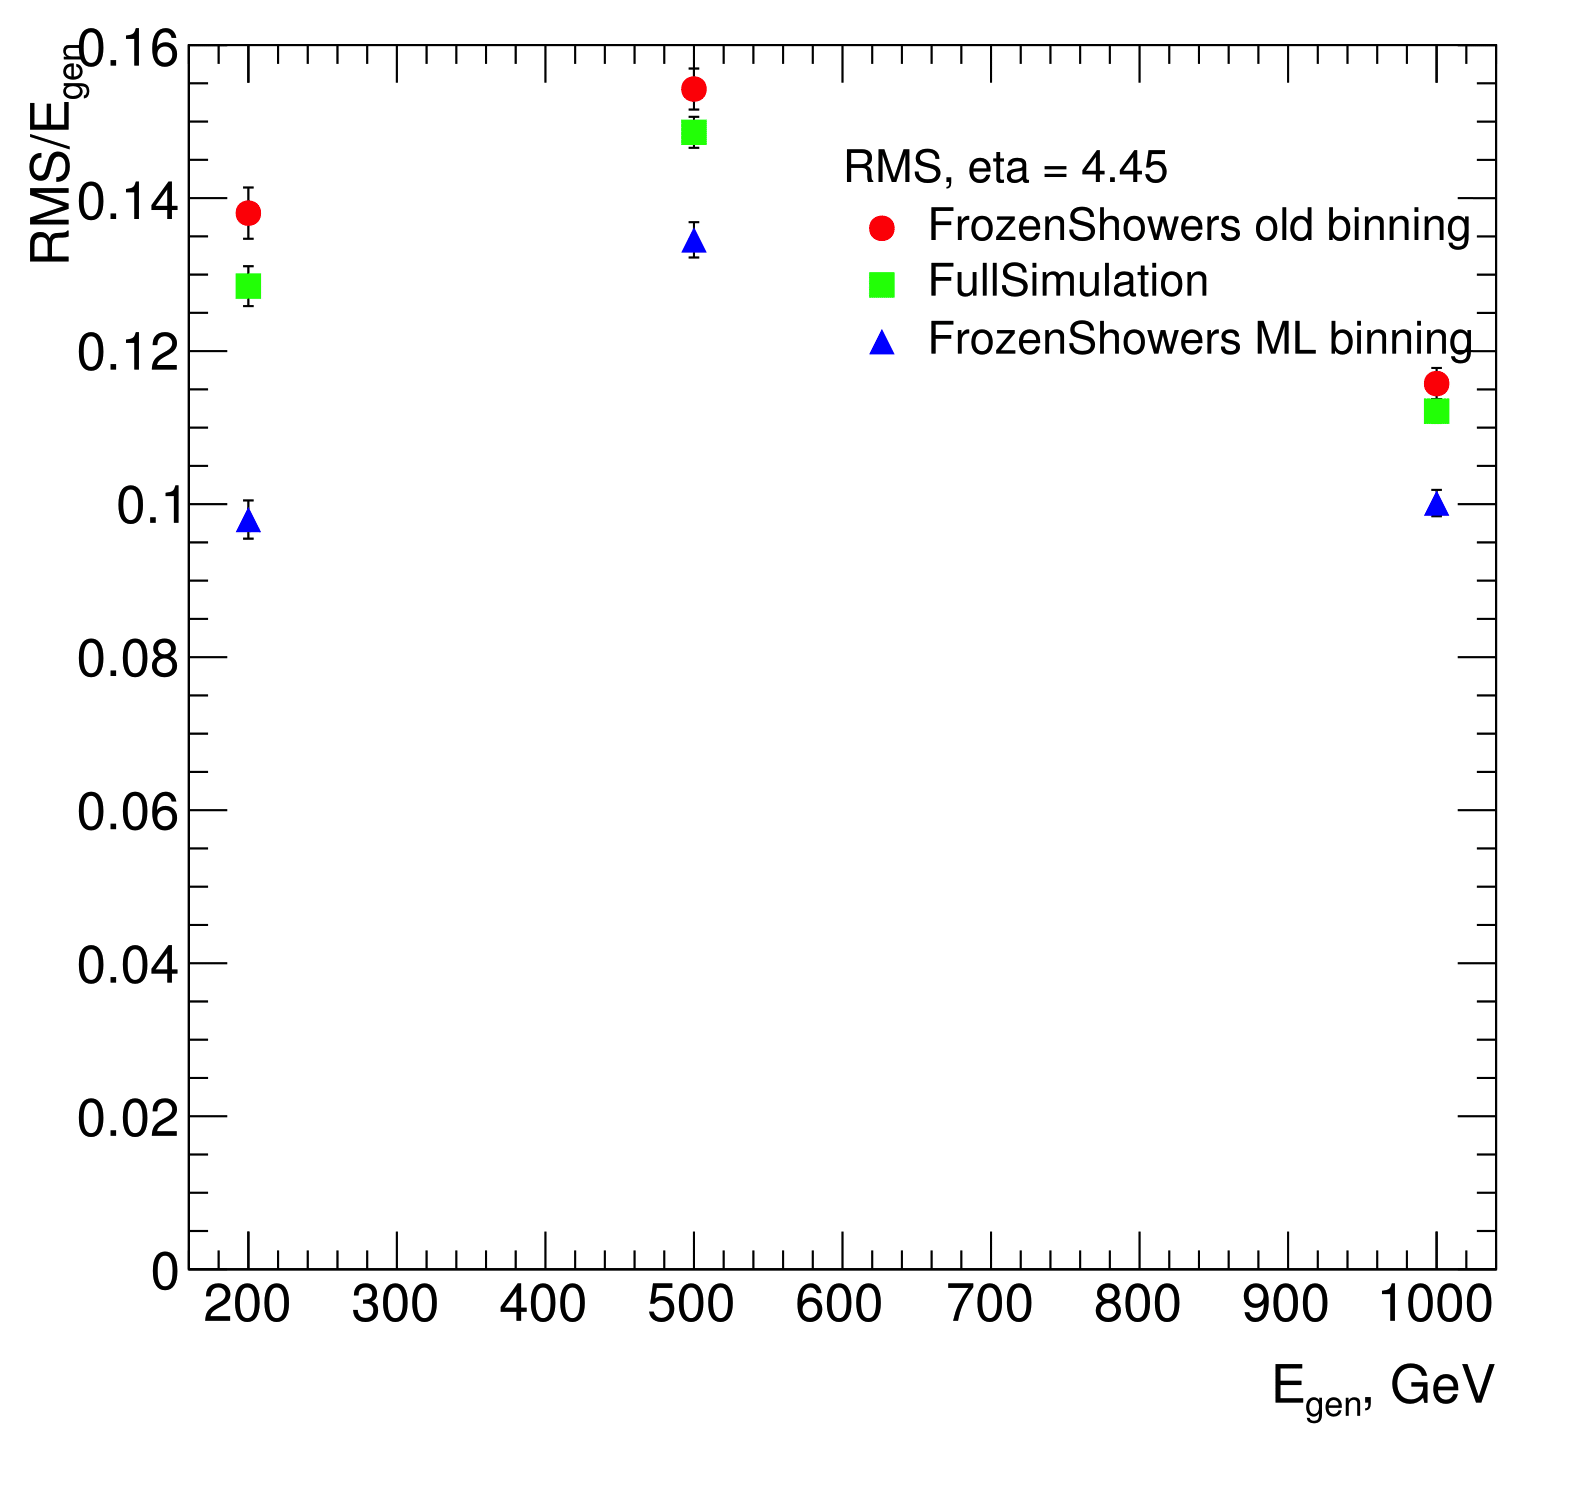
\includegraphics[width=1.\linewidth]{MC/RMS/RMS-02.png} }
\end{minipage}
\hfill
\begin{minipage}[h]{0.32\linewidth}
\center{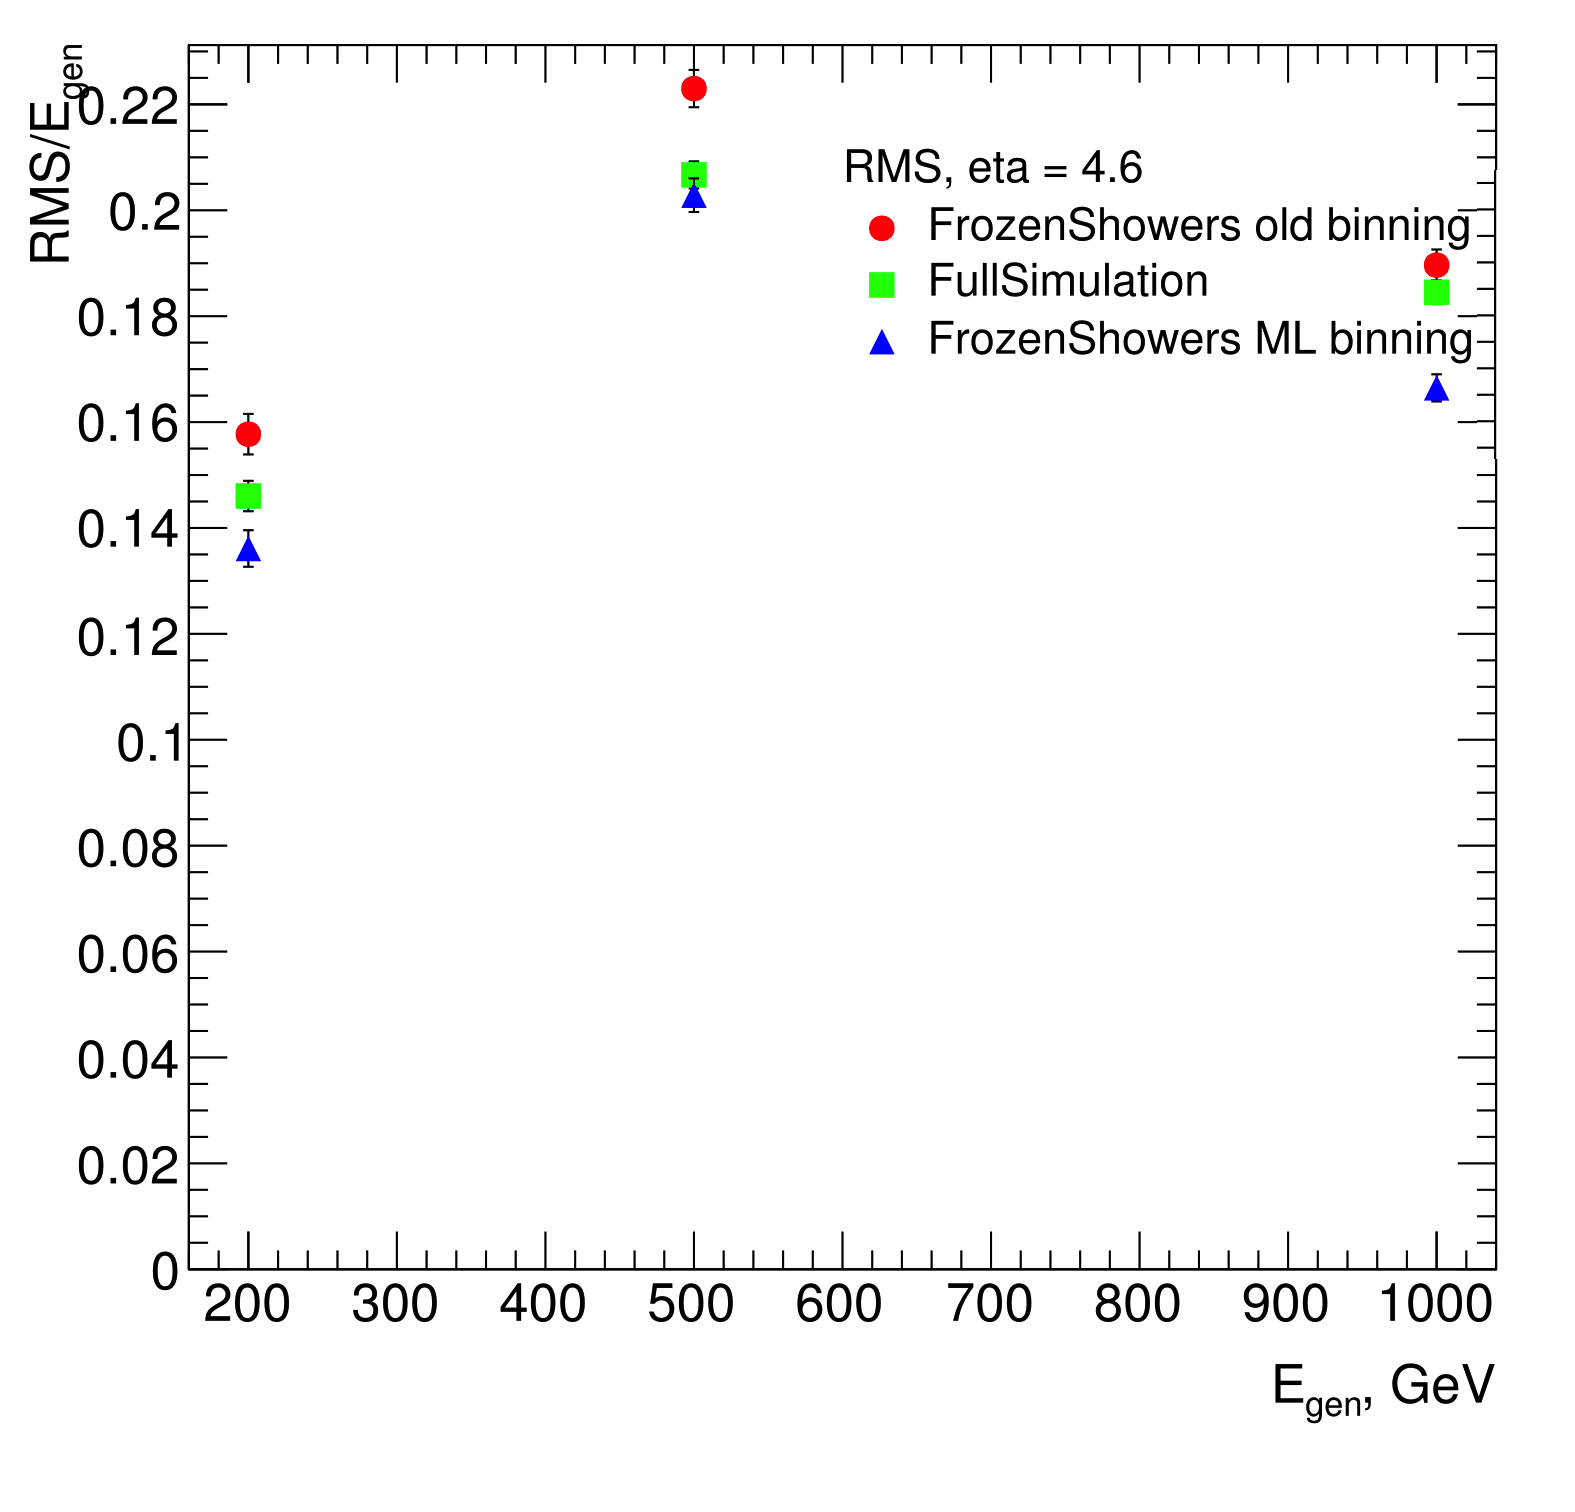
\includegraphics[width=1.\linewidth]{MC/RMS/RMS-01.png} }
\end{minipage}
\caption{Energy resolution of reconstructed electrons for full simulation, new libraries with ML binning and old tuned libraries with original binning for different $\eta$ bins }
\label{fig:Reso}
\end{figure}

\begin{figure}[!tbp]
\begin{minipage}[h]{0.32\linewidth}
\center{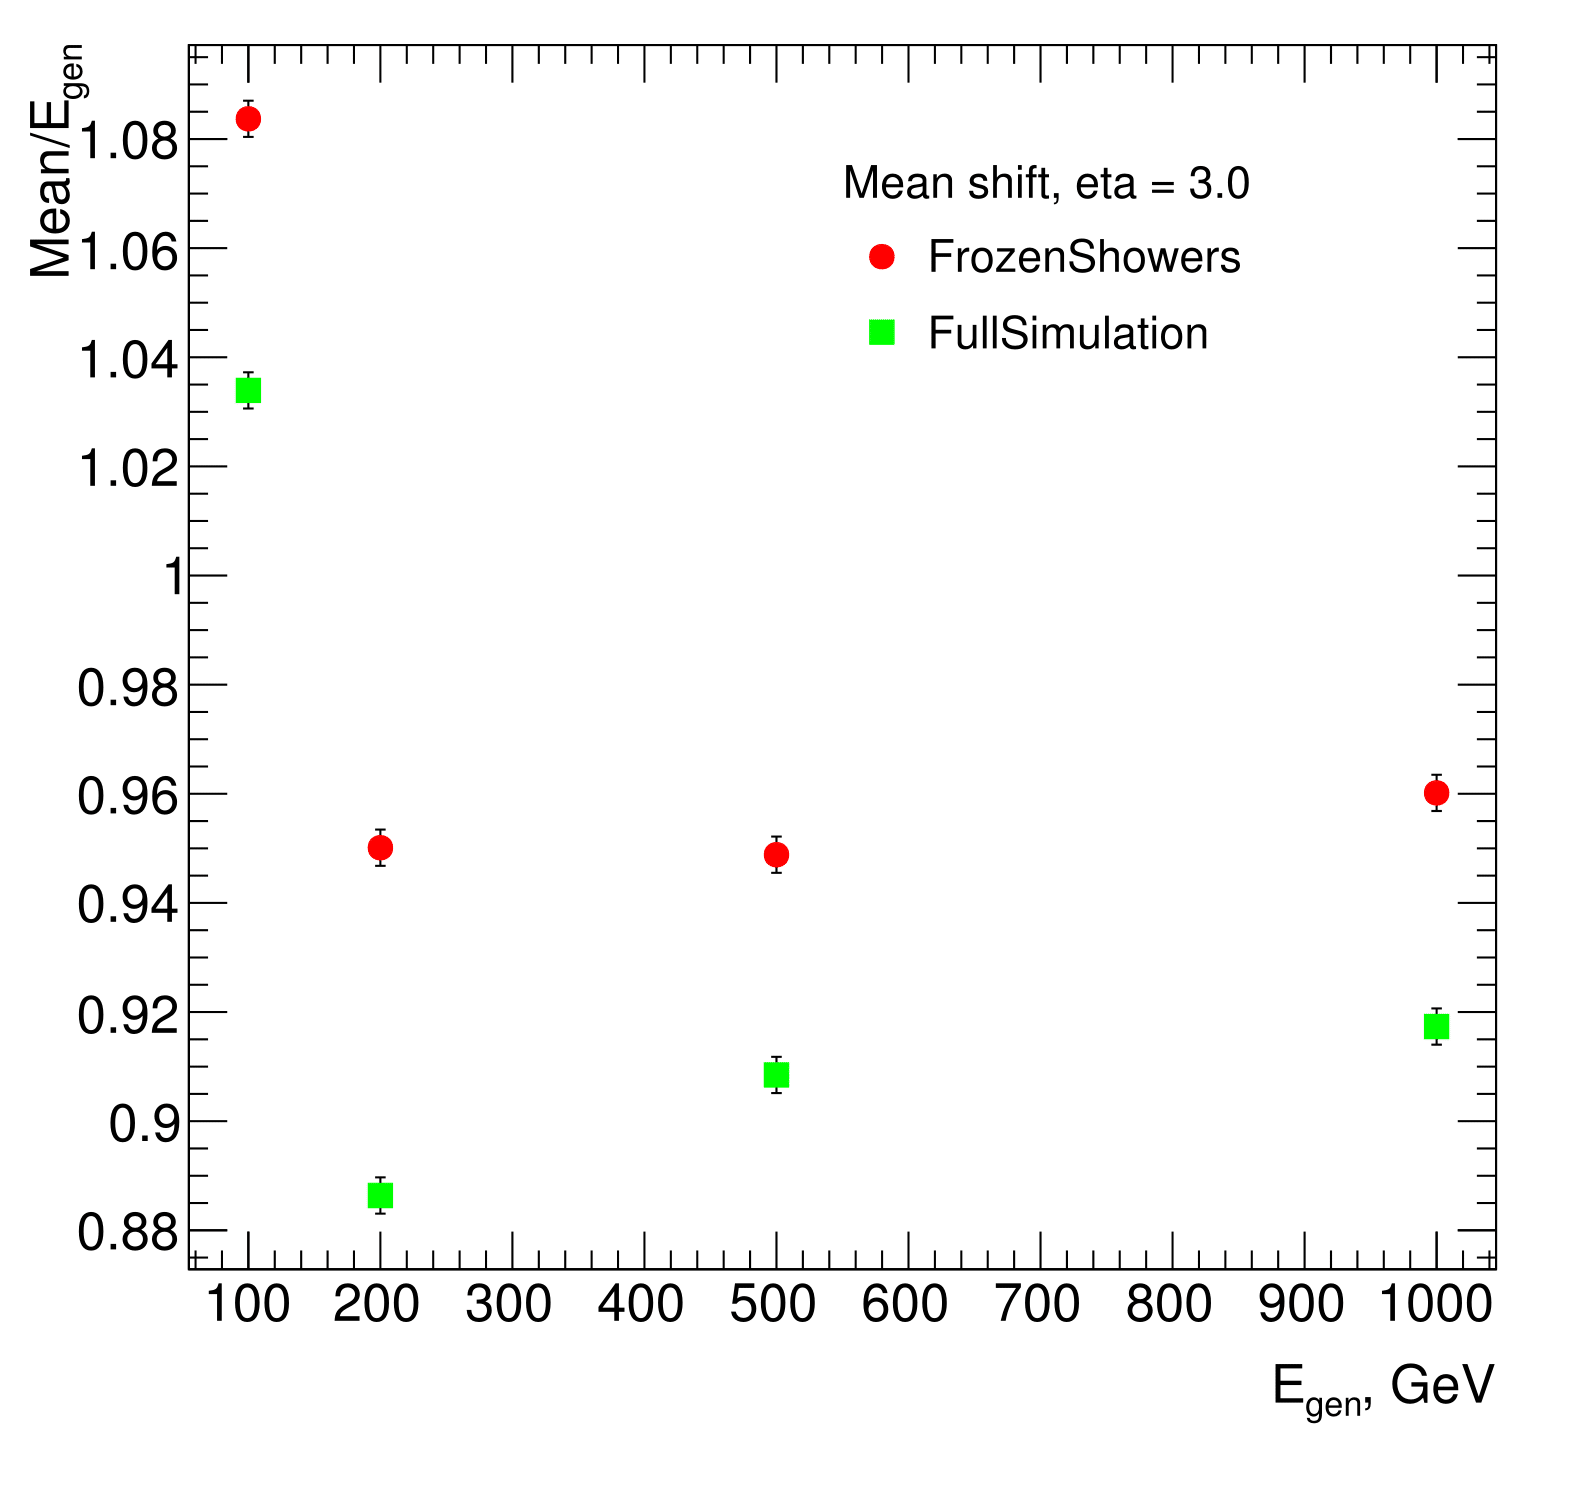
\includegraphics[width=1.\linewidth]{MC/Mean/Mean-12.png} }
\end{minipage}
\hfill
\begin{minipage}[h]{0.32\linewidth}
\center{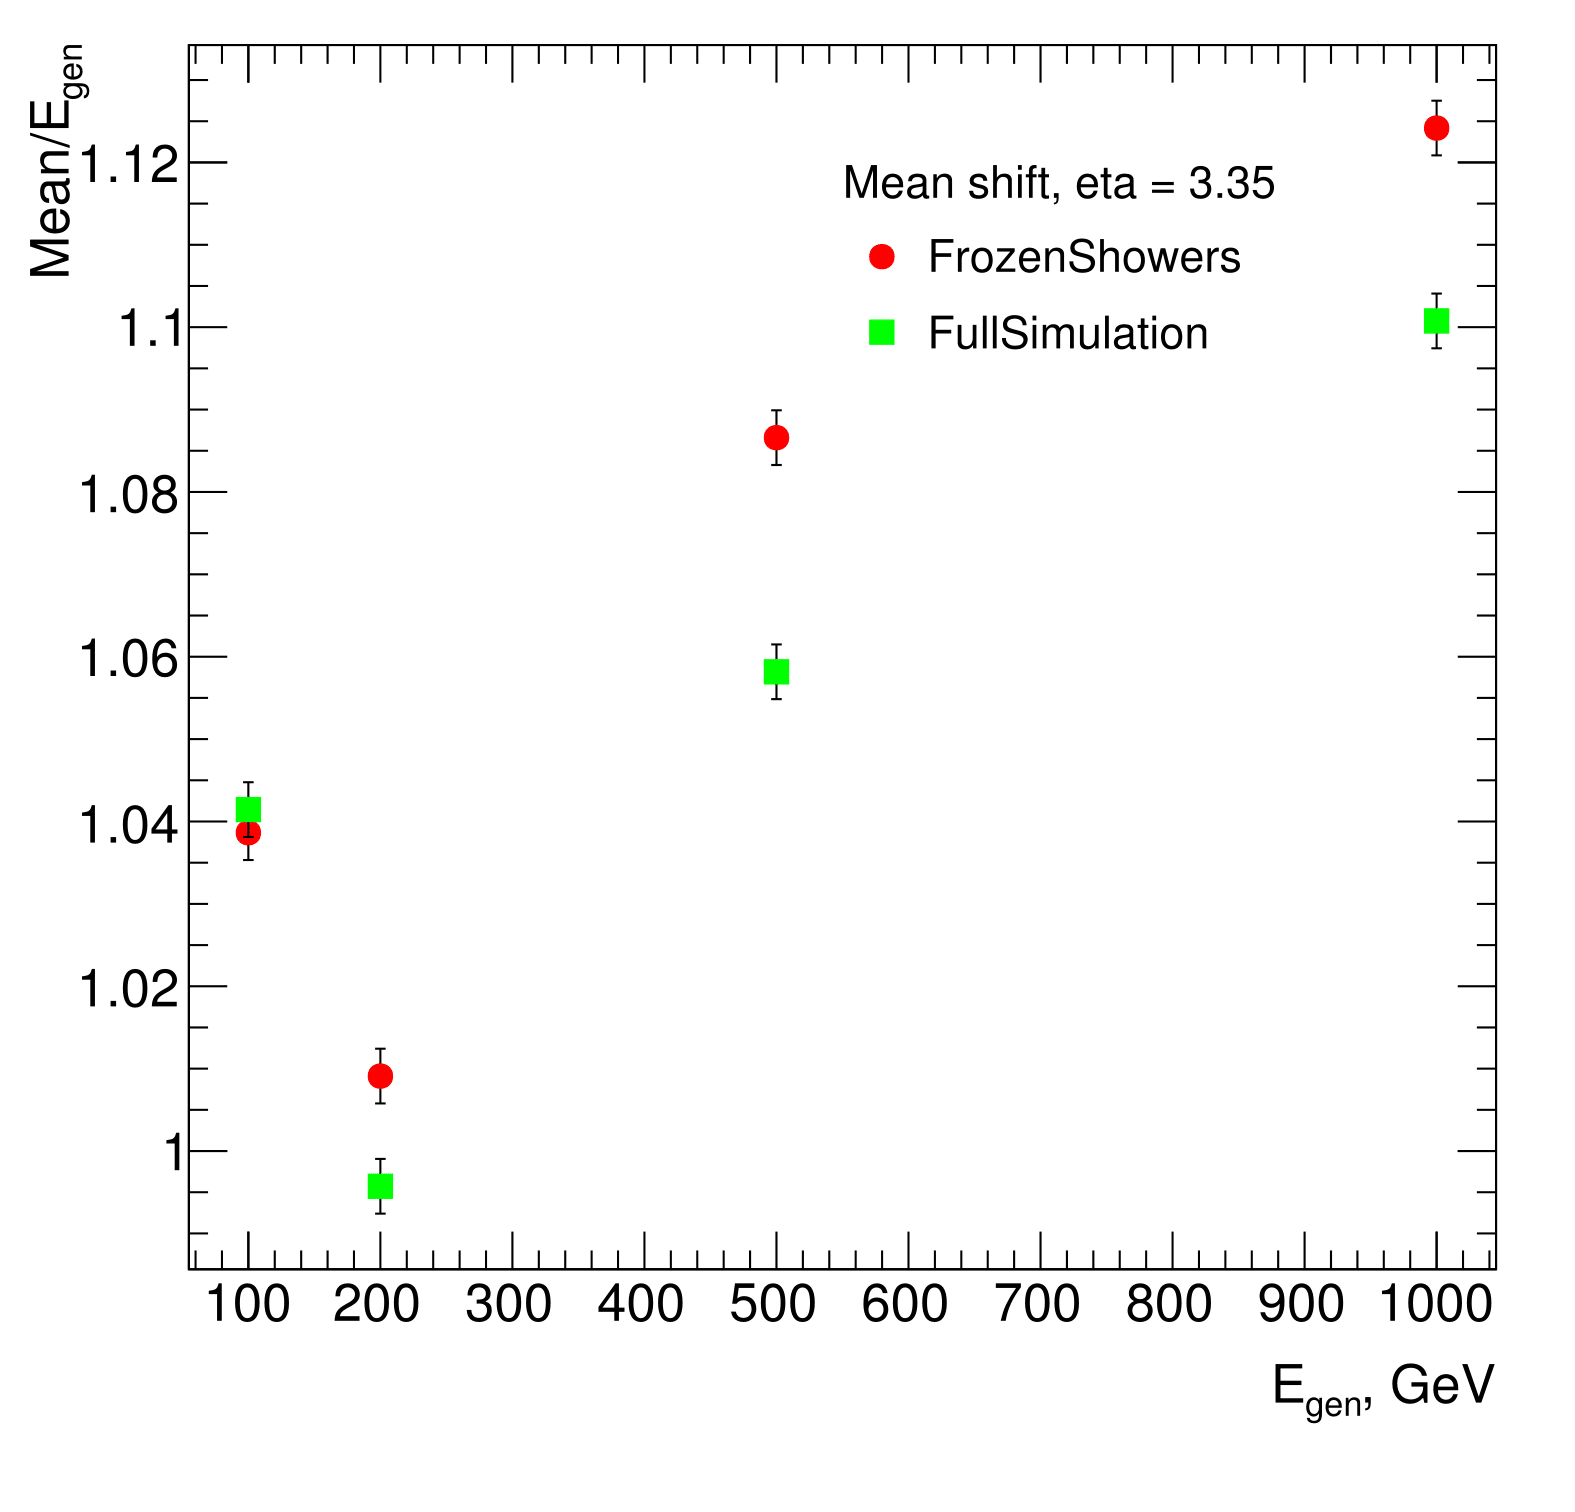
\includegraphics[width=1.\linewidth]{MC/Mean/Mean-11.png}  }
\end{minipage}
\hfill
\begin{minipage}[h]{0.32\linewidth}
\center{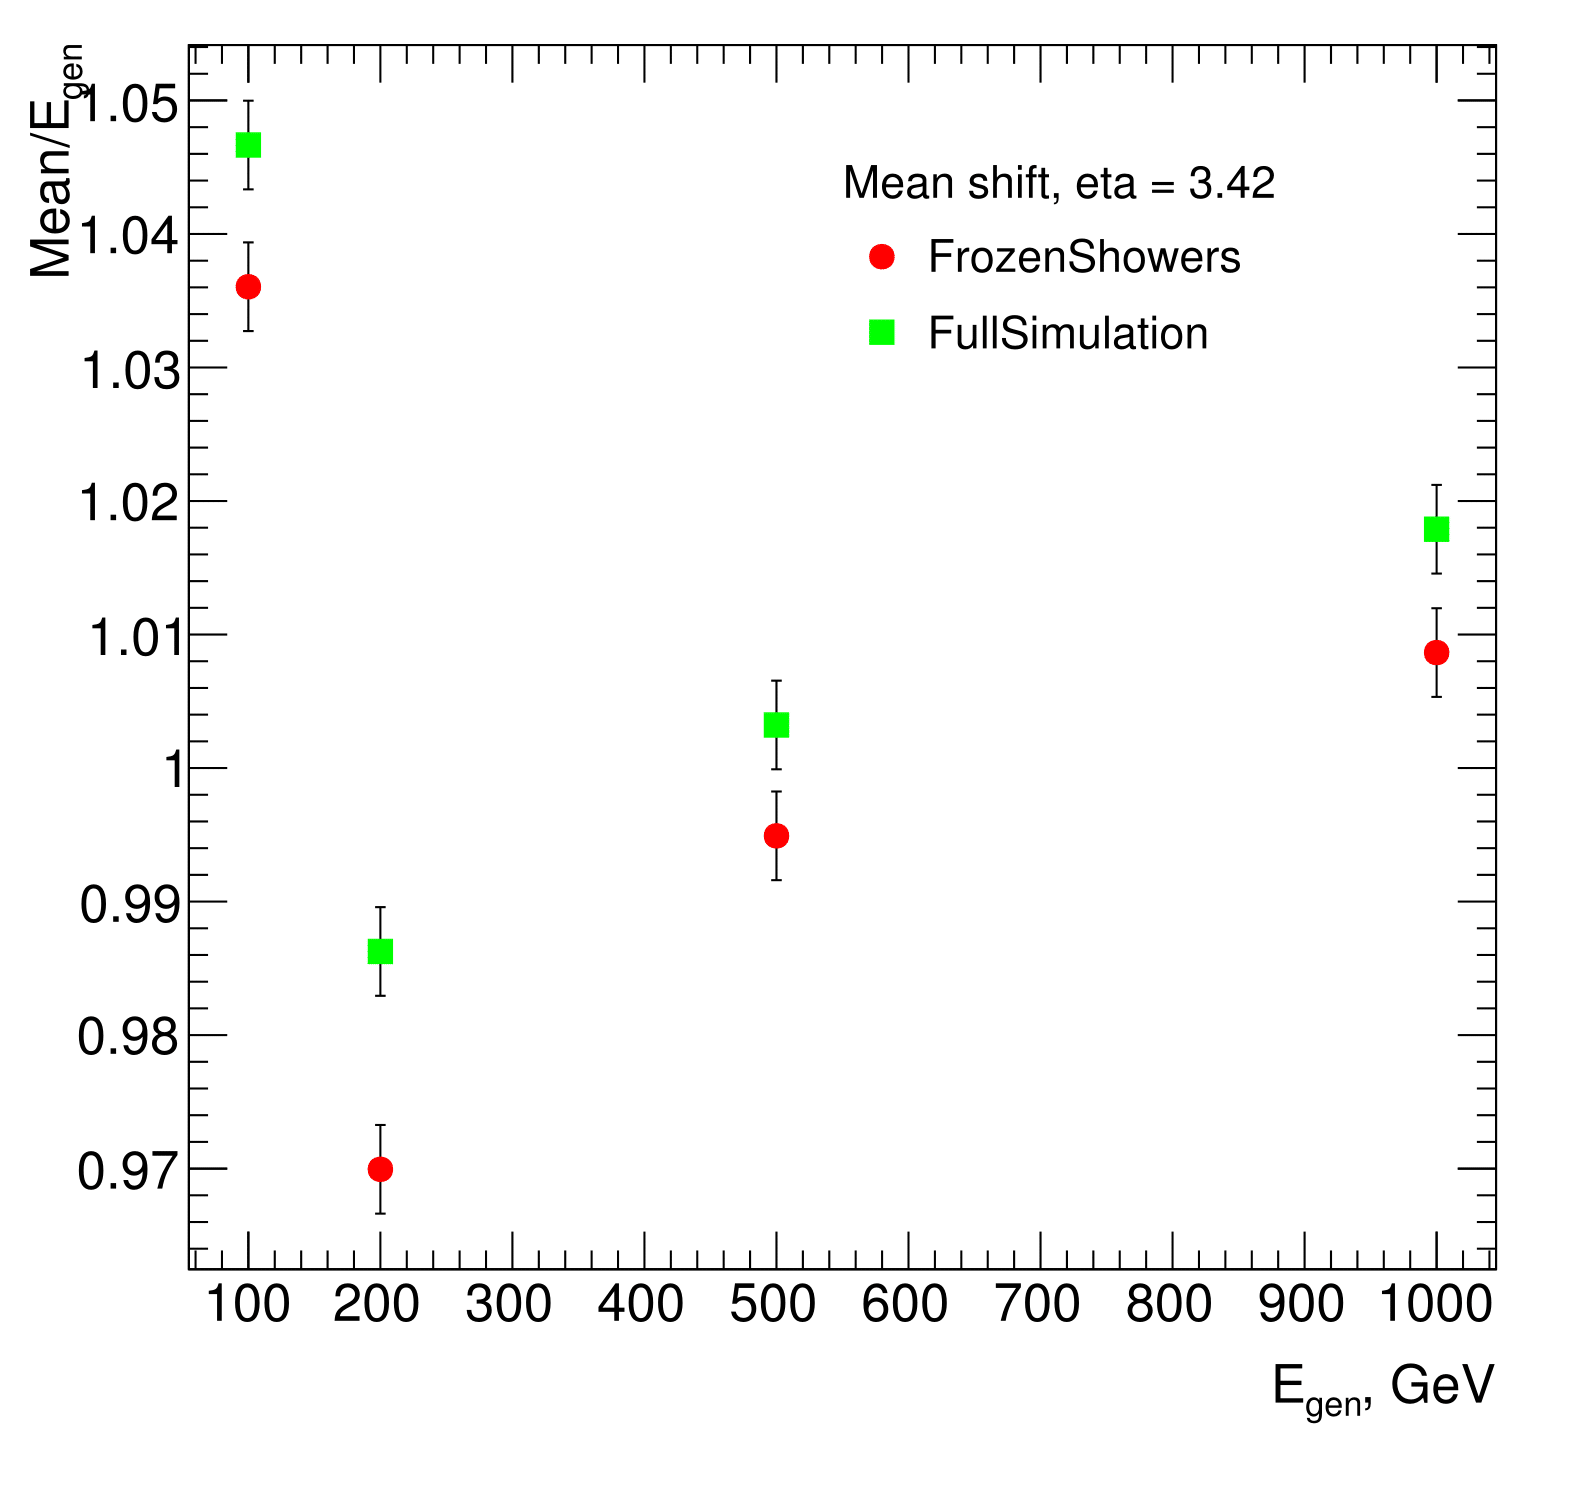
\includegraphics[width=1.\linewidth]{MC/Mean/Mean-10.png}  }
\end{minipage}
\vfill
\begin{minipage}[h]{0.32\linewidth}
\center{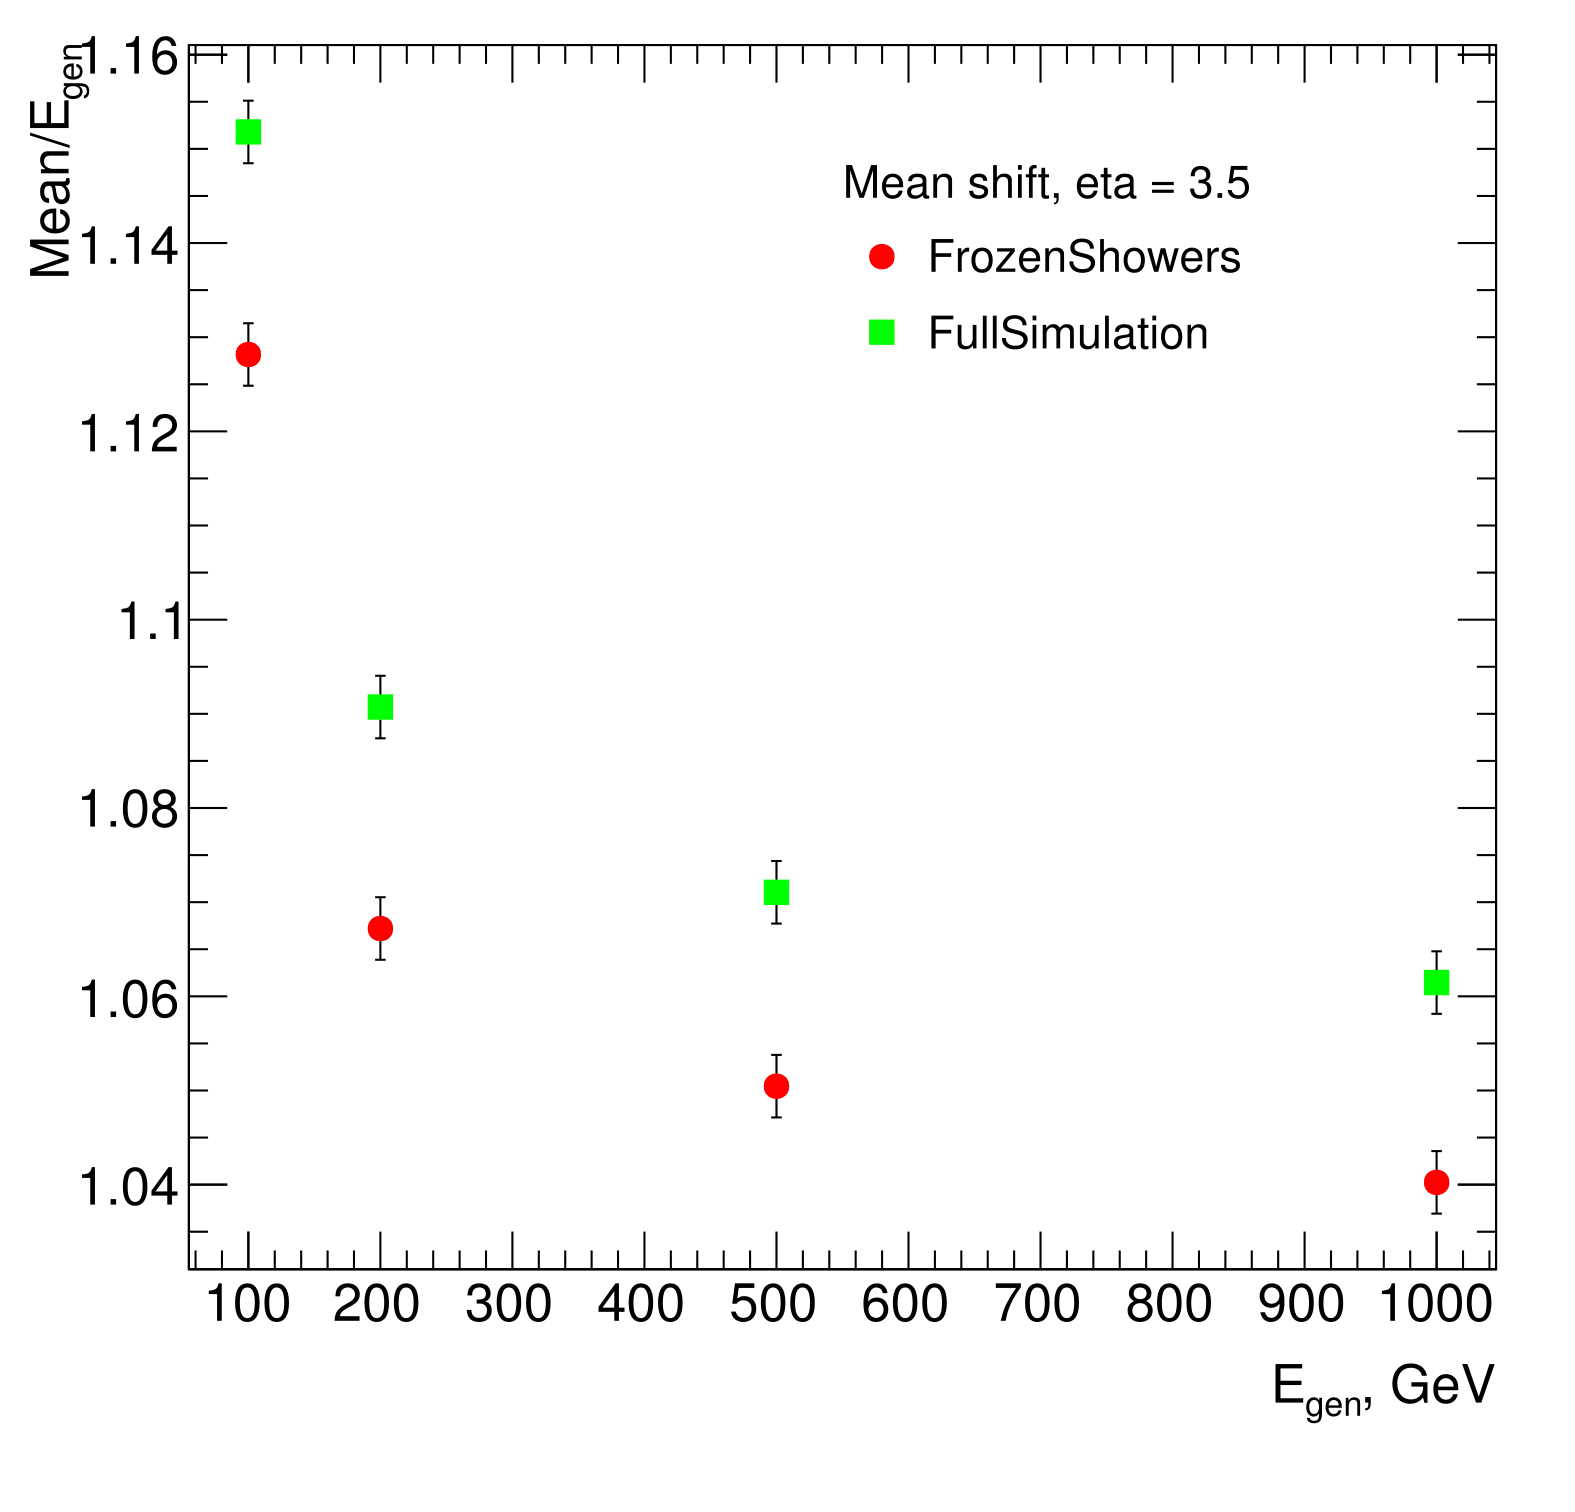
\includegraphics[width=1.\linewidth]{MC/Mean/Mean-09.png}  }
\end{minipage}
\hfill
\begin{minipage}[h]{0.32\linewidth}
\center{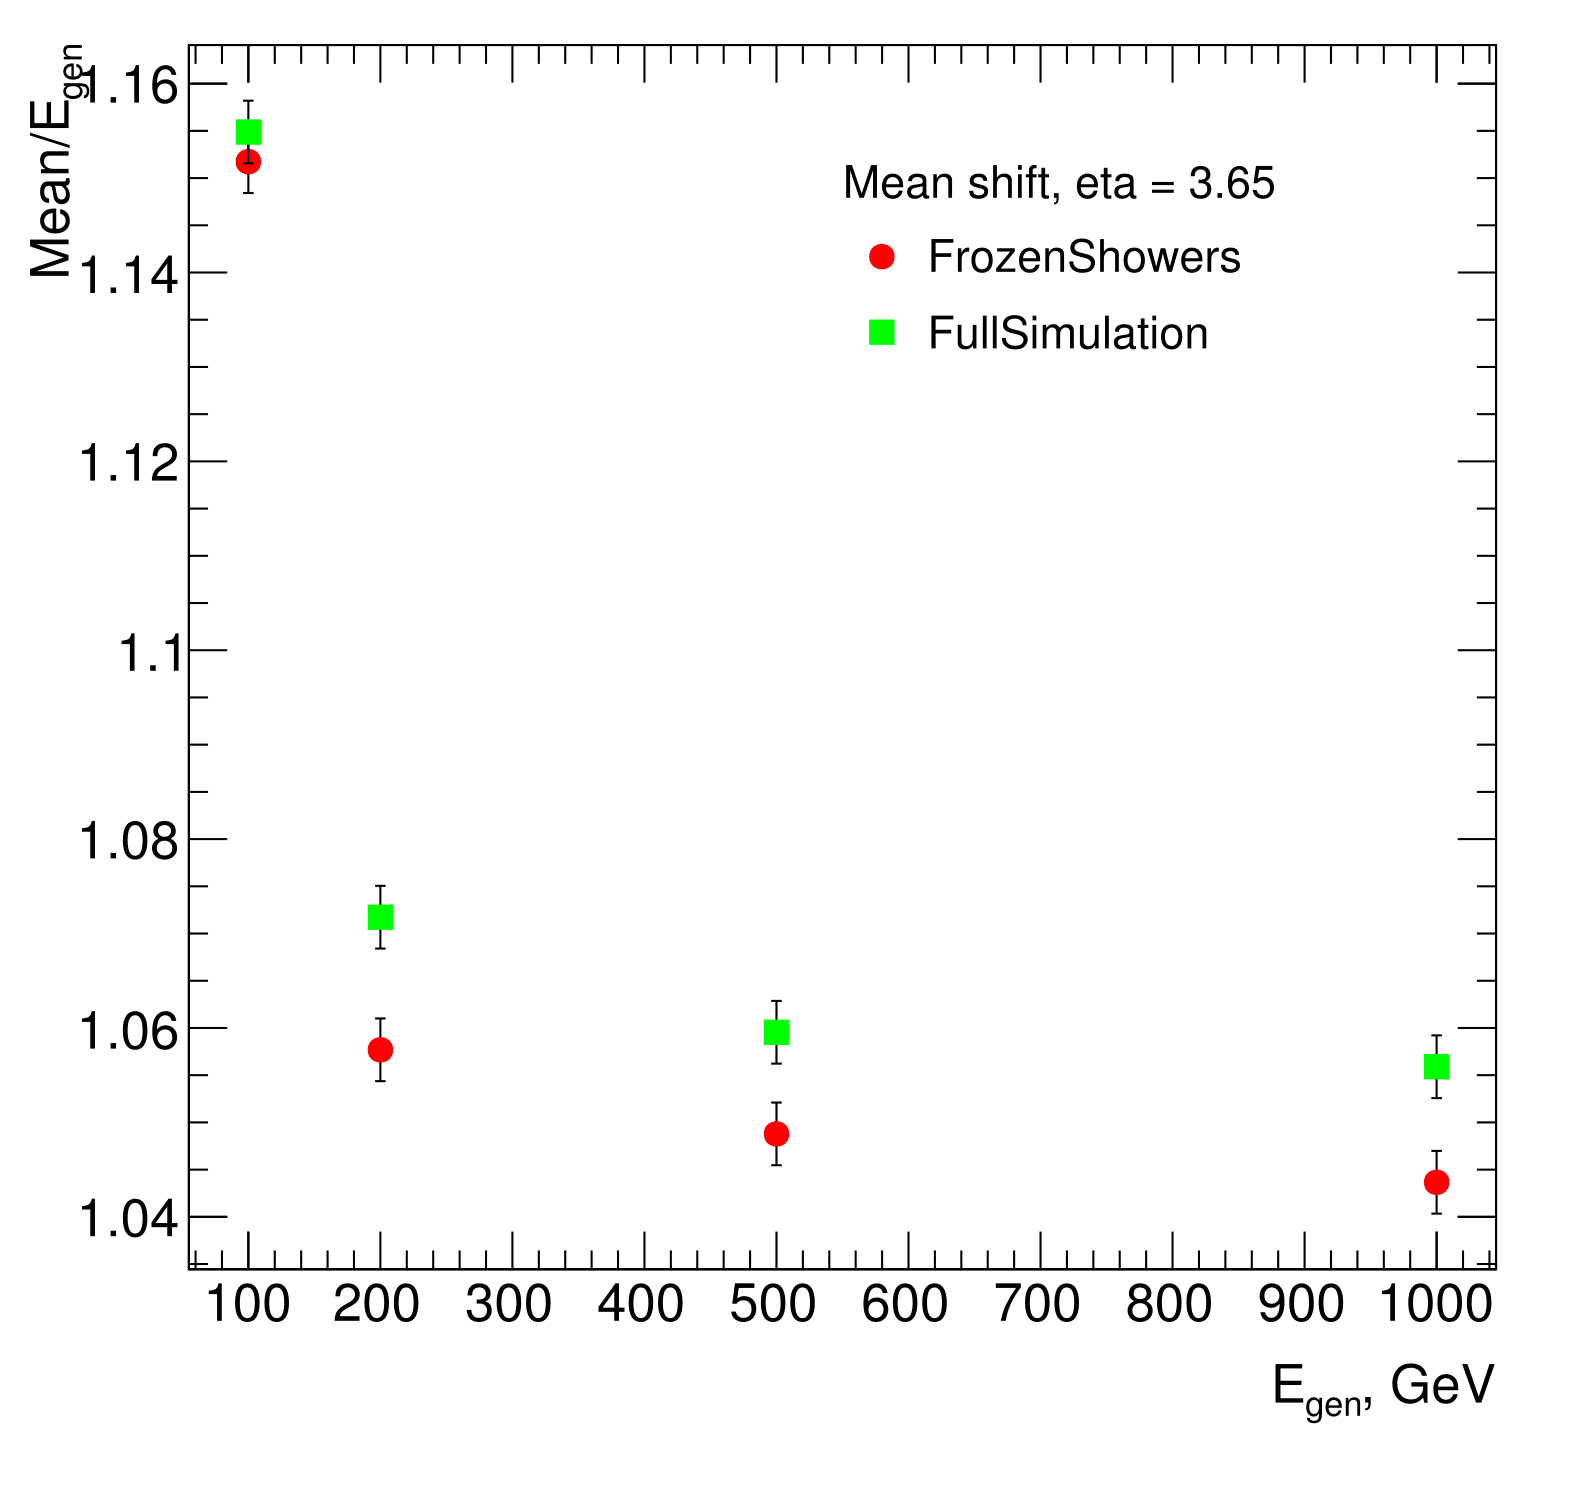
\includegraphics[width=1.\linewidth]{MC/Mean/Mean-08.png}  }
\end{minipage}
\hfill
\begin{minipage}[h]{0.32\linewidth}
\center{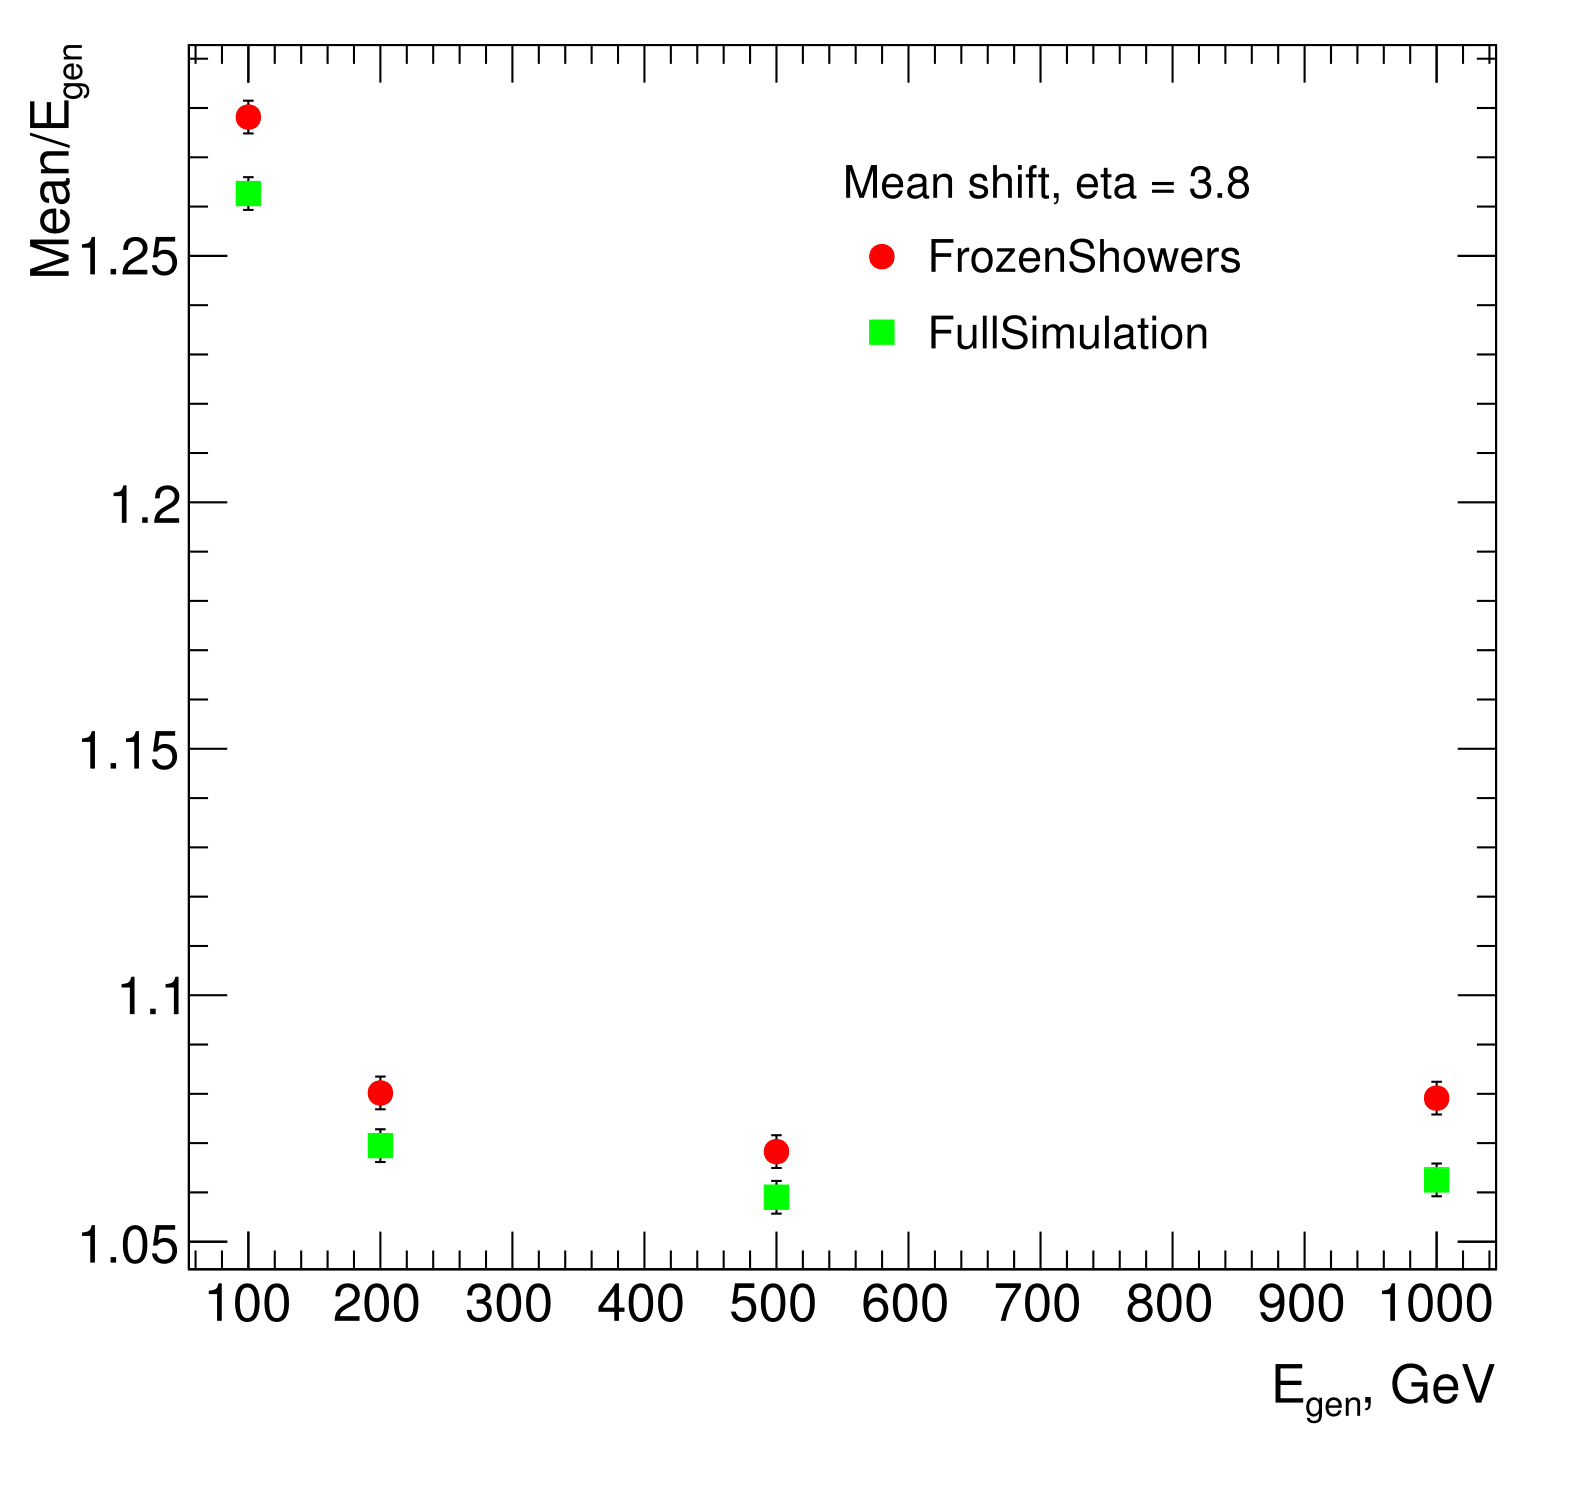
\includegraphics[width=1.\linewidth]{MC/Mean/Mean-07.png}  }
\end{minipage}
\vfill
\begin{minipage}[h]{0.32\linewidth}
\center{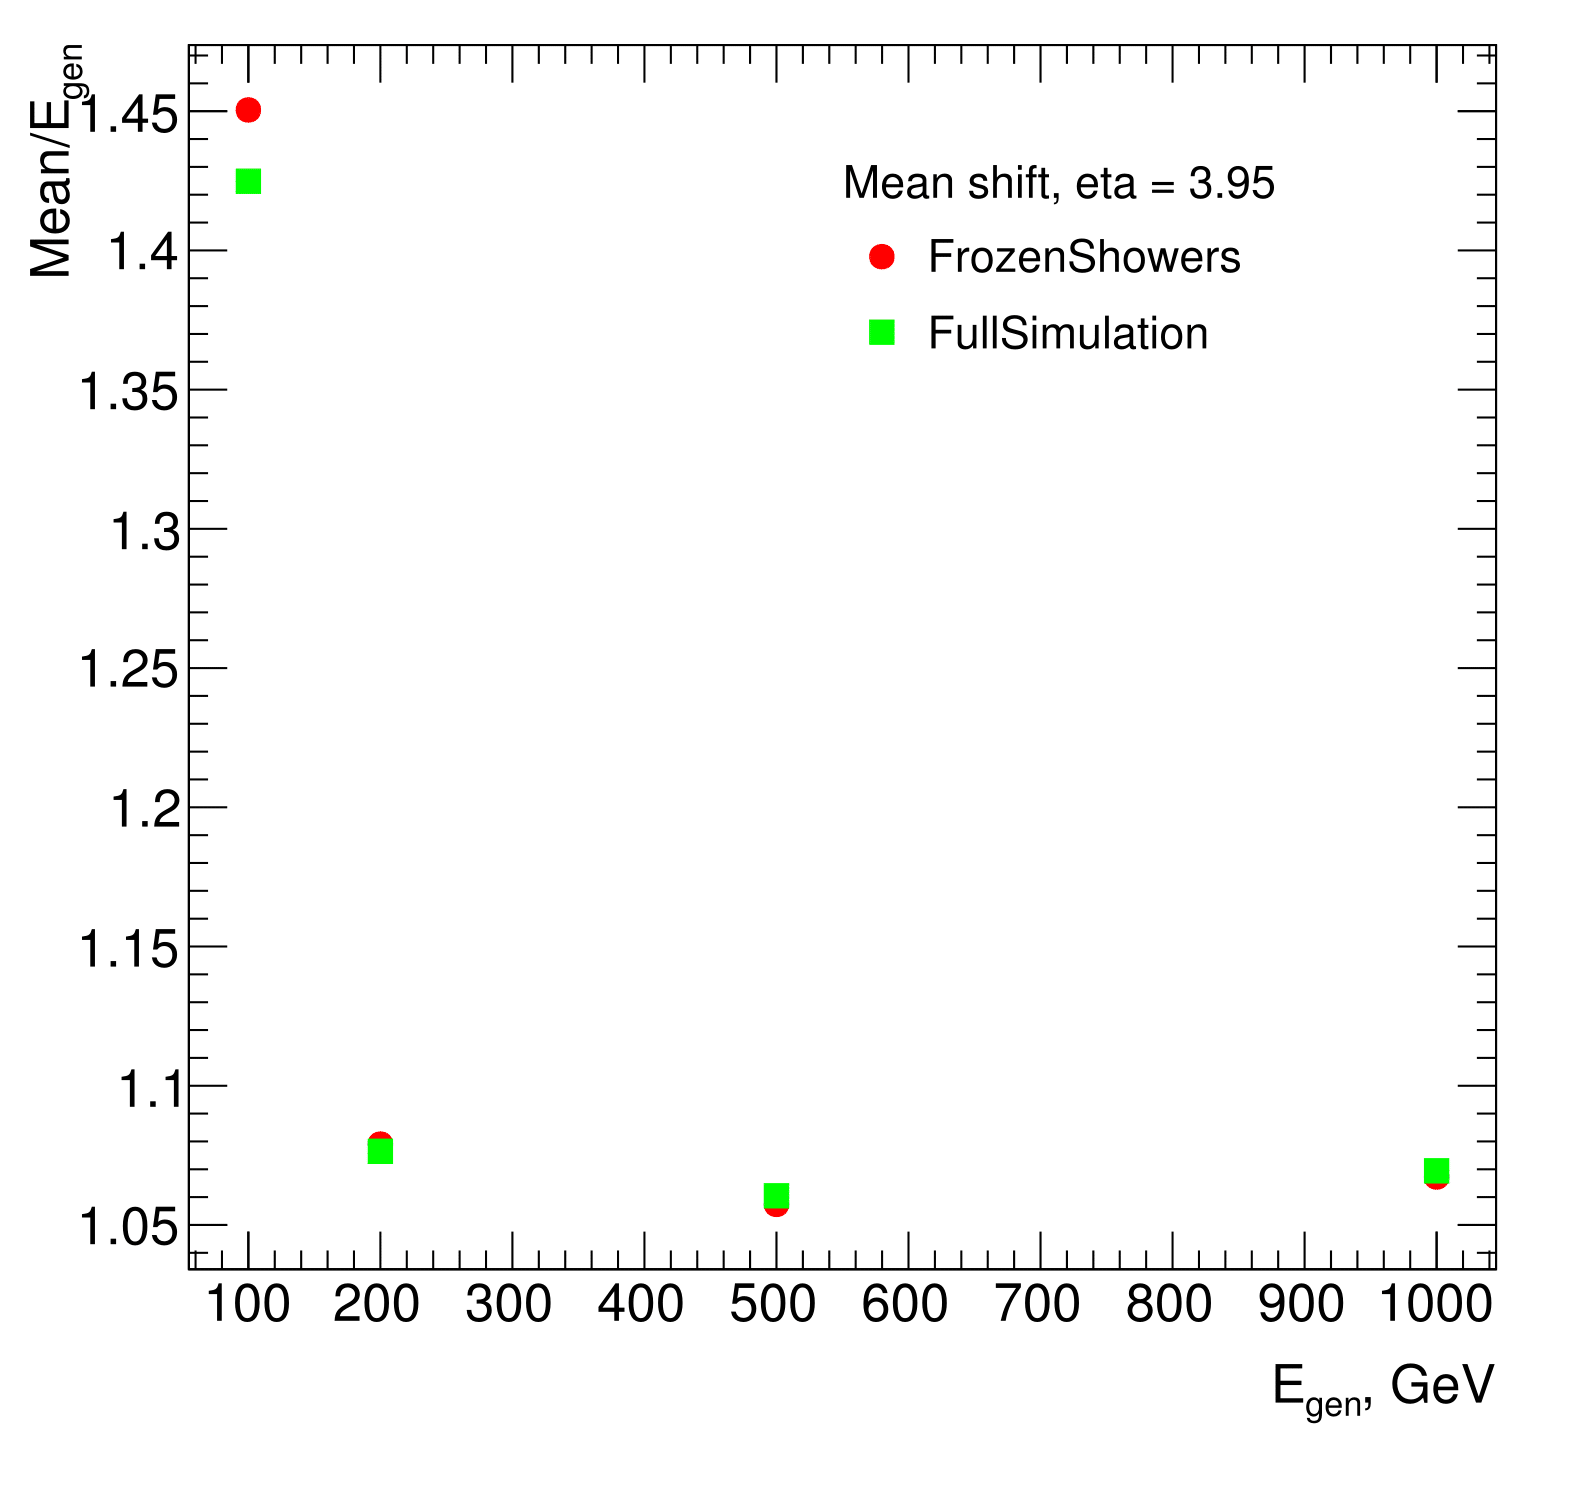
\includegraphics[width=1.\linewidth]{MC/Mean/Mean-06.png}  }
\end{minipage}
\hfill
\begin{minipage}[h]{0.32\linewidth}
\center{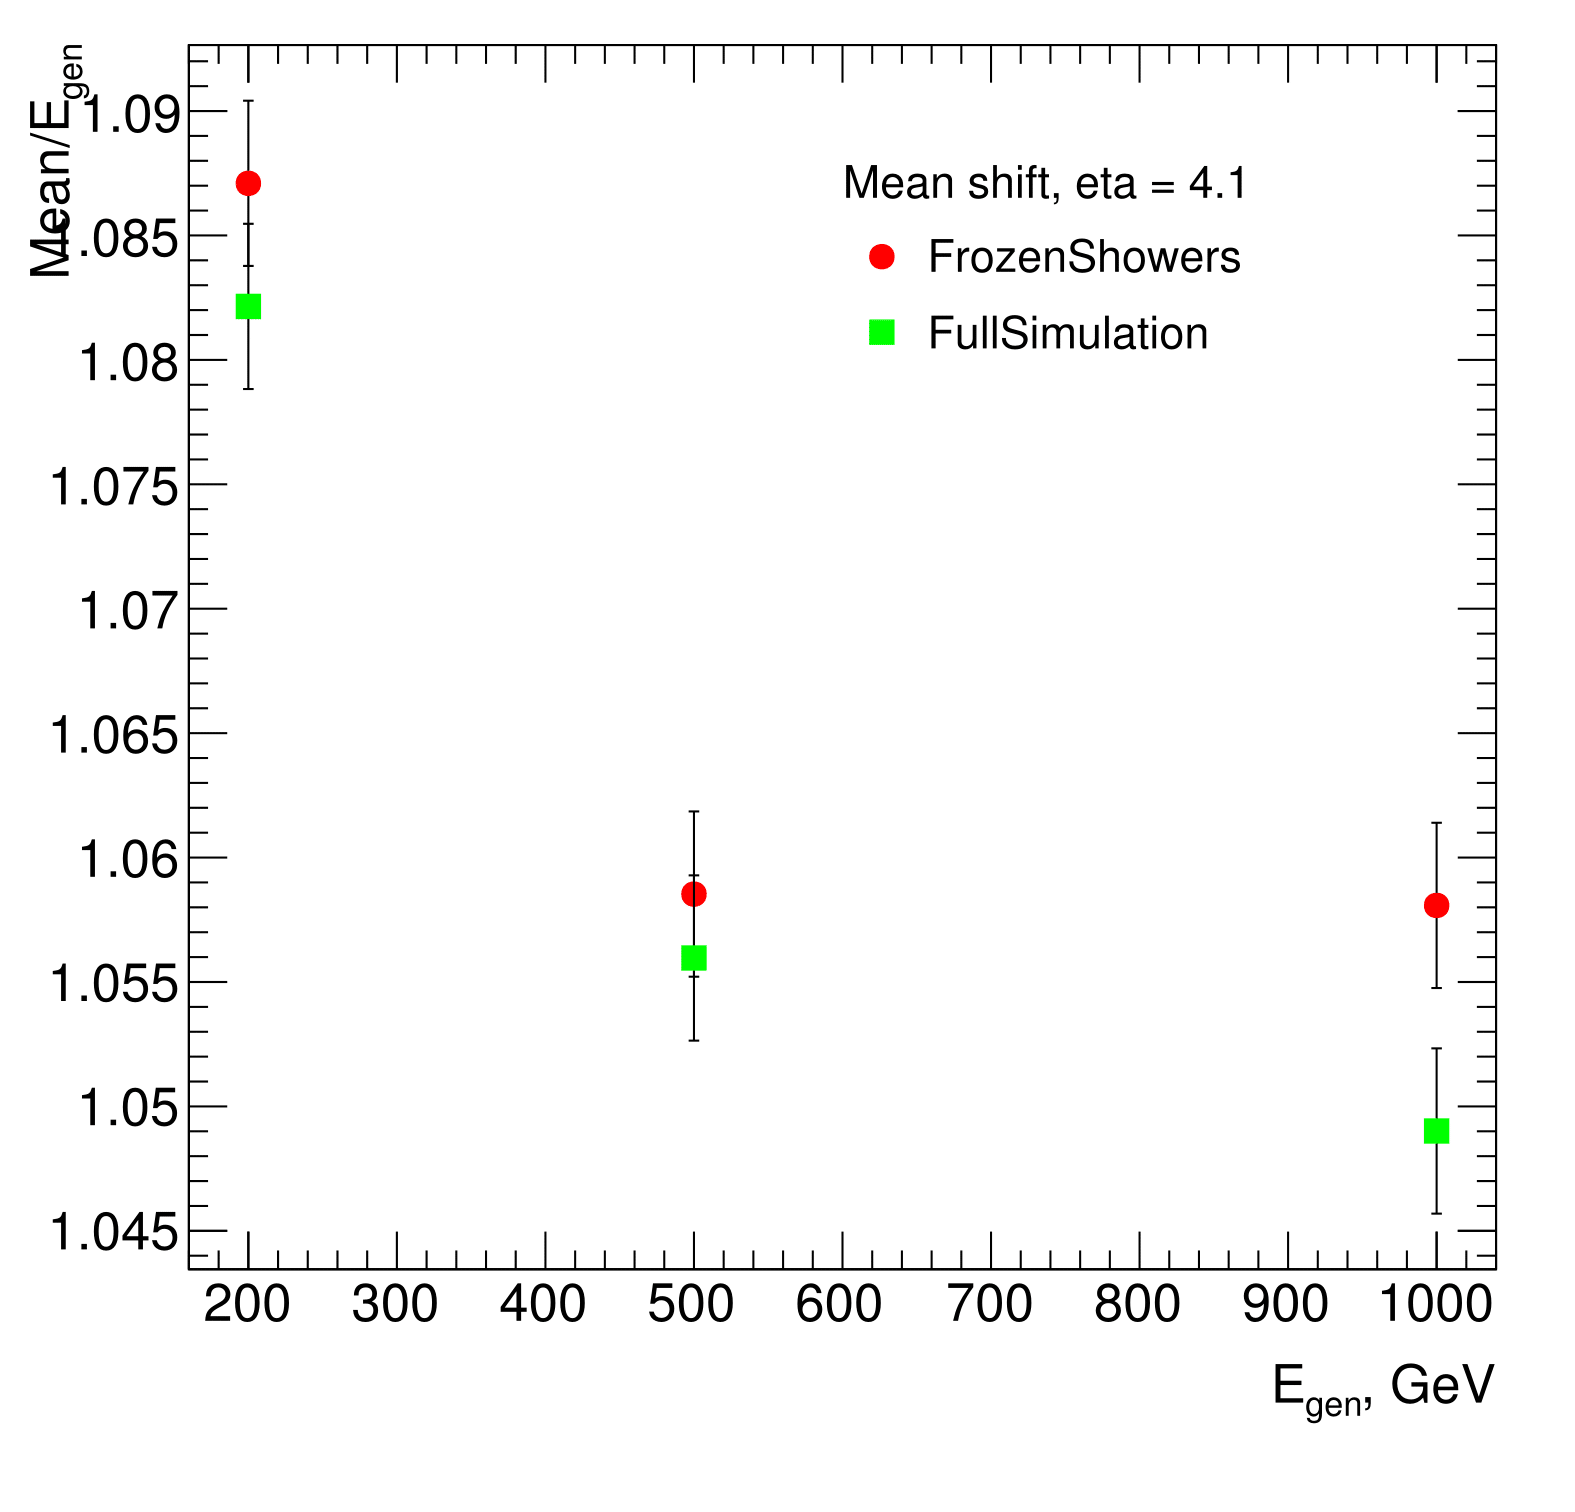
\includegraphics[width=1.\linewidth]{MC/Mean/Mean-05.png}  }
\end{minipage}
\hfill
\begin{minipage}[h]{0.32\linewidth}
\center{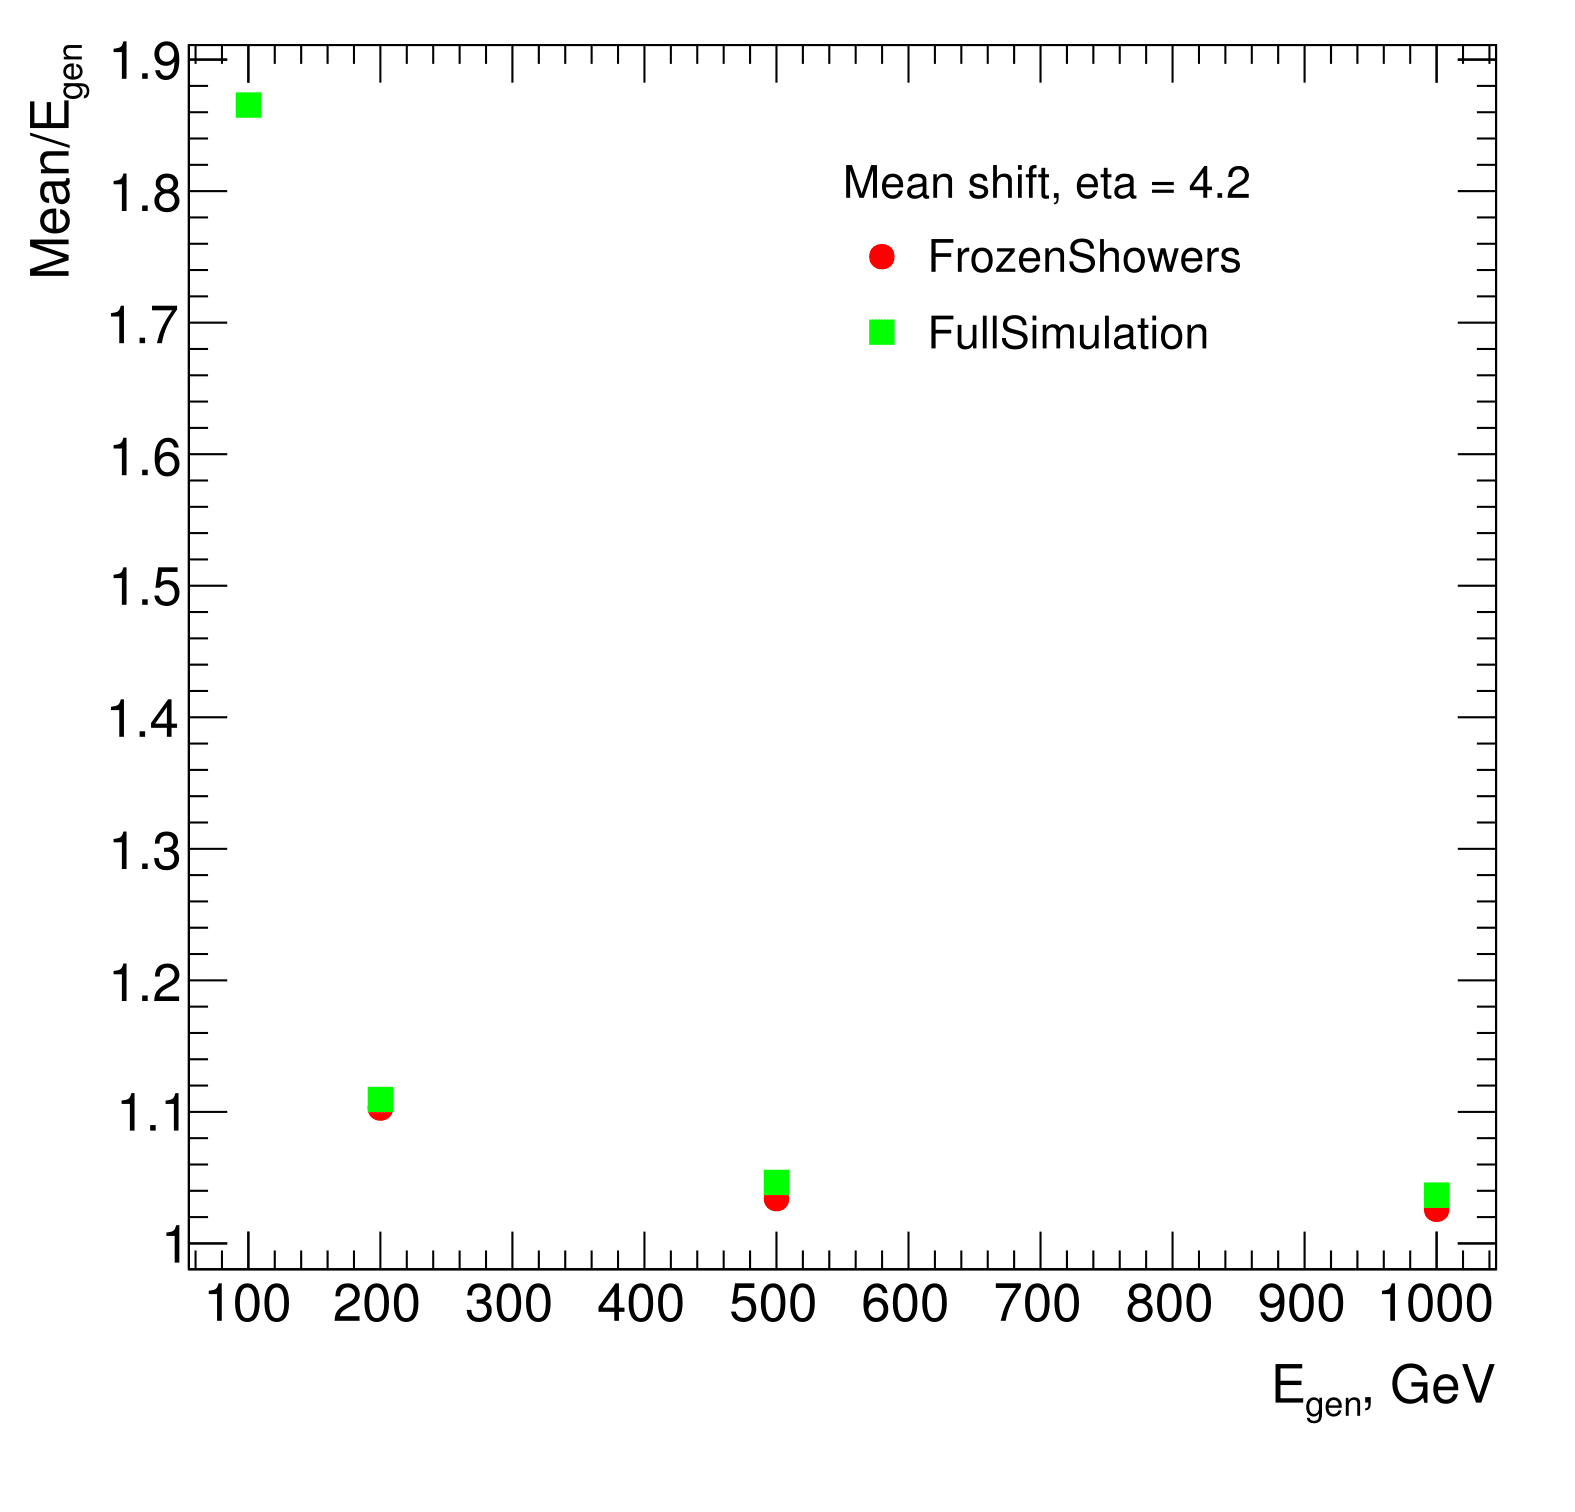
\includegraphics[width=1.\linewidth]{MC/Mean/Mean-04.png}  }
\end{minipage}
\vfill
\begin{minipage}[h]{0.32\linewidth}
\center{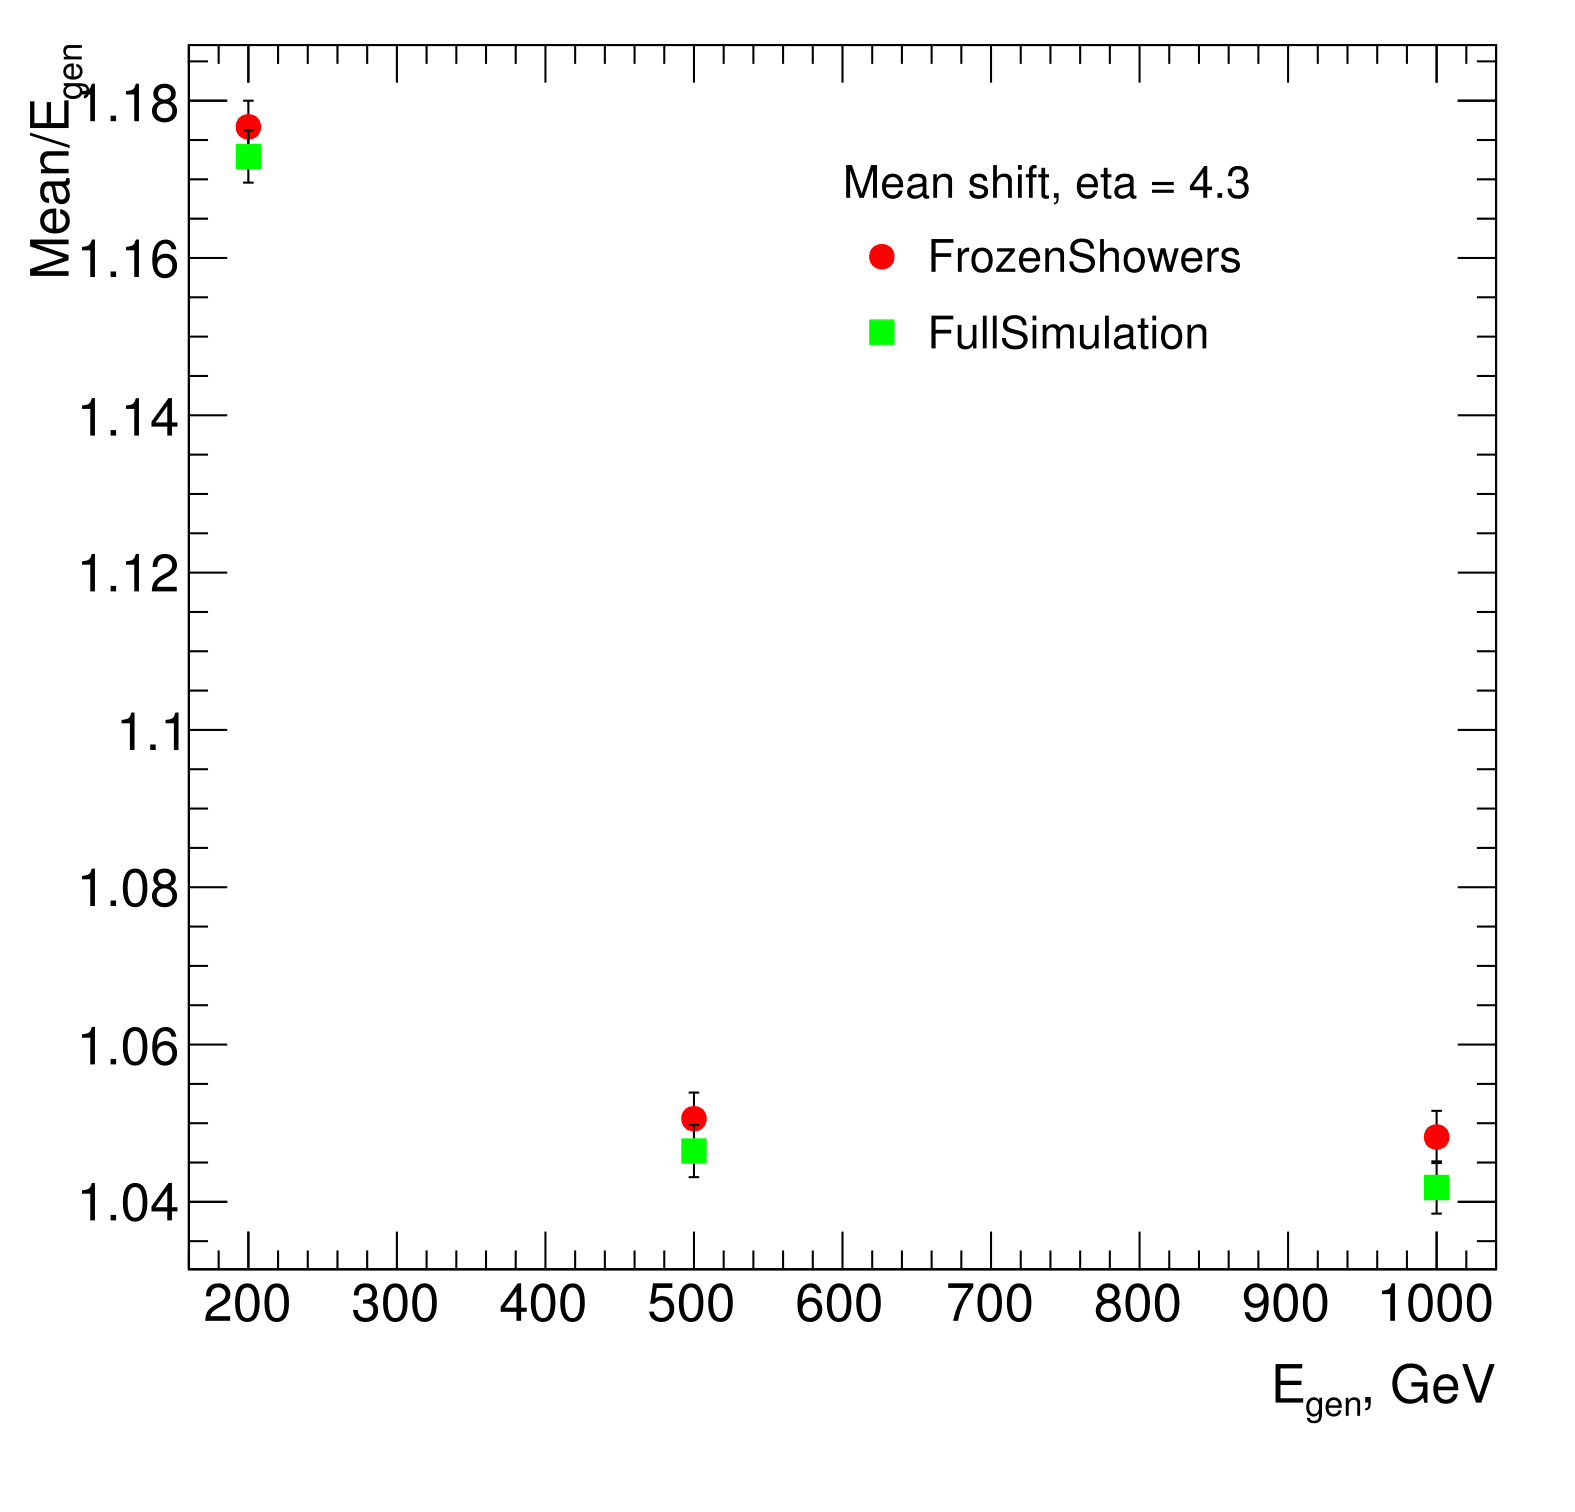
\includegraphics[width=1.\linewidth]{MC/Mean/Mean-03.png}  }
\end{minipage}
\hfill
\begin{minipage}[h]{0.32\linewidth}
\center{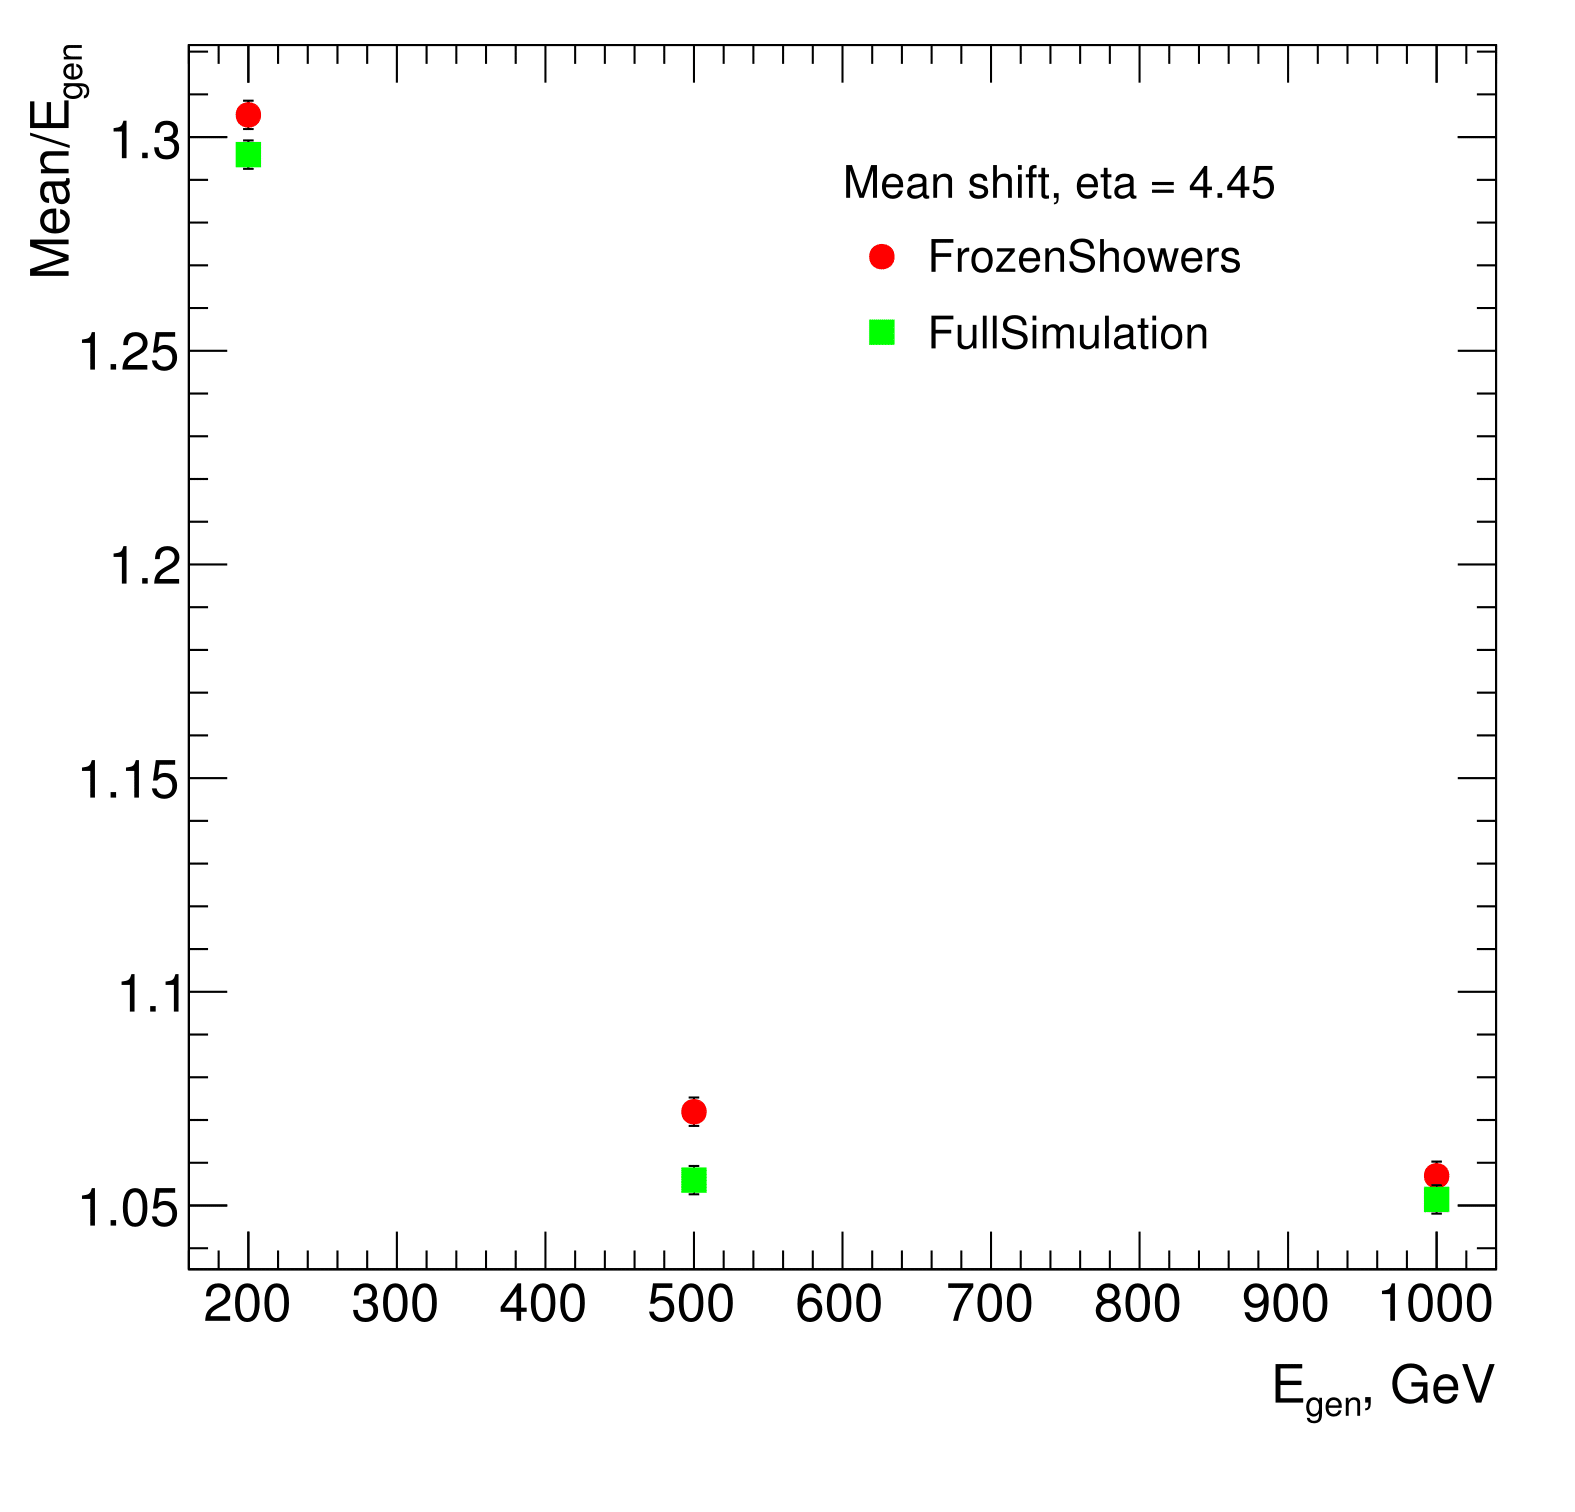
\includegraphics[width=1.\linewidth]{MC/Mean/Mean-02.png}  }
\end{minipage}
\hfill
\begin{minipage}[h]{0.32\linewidth}
\center{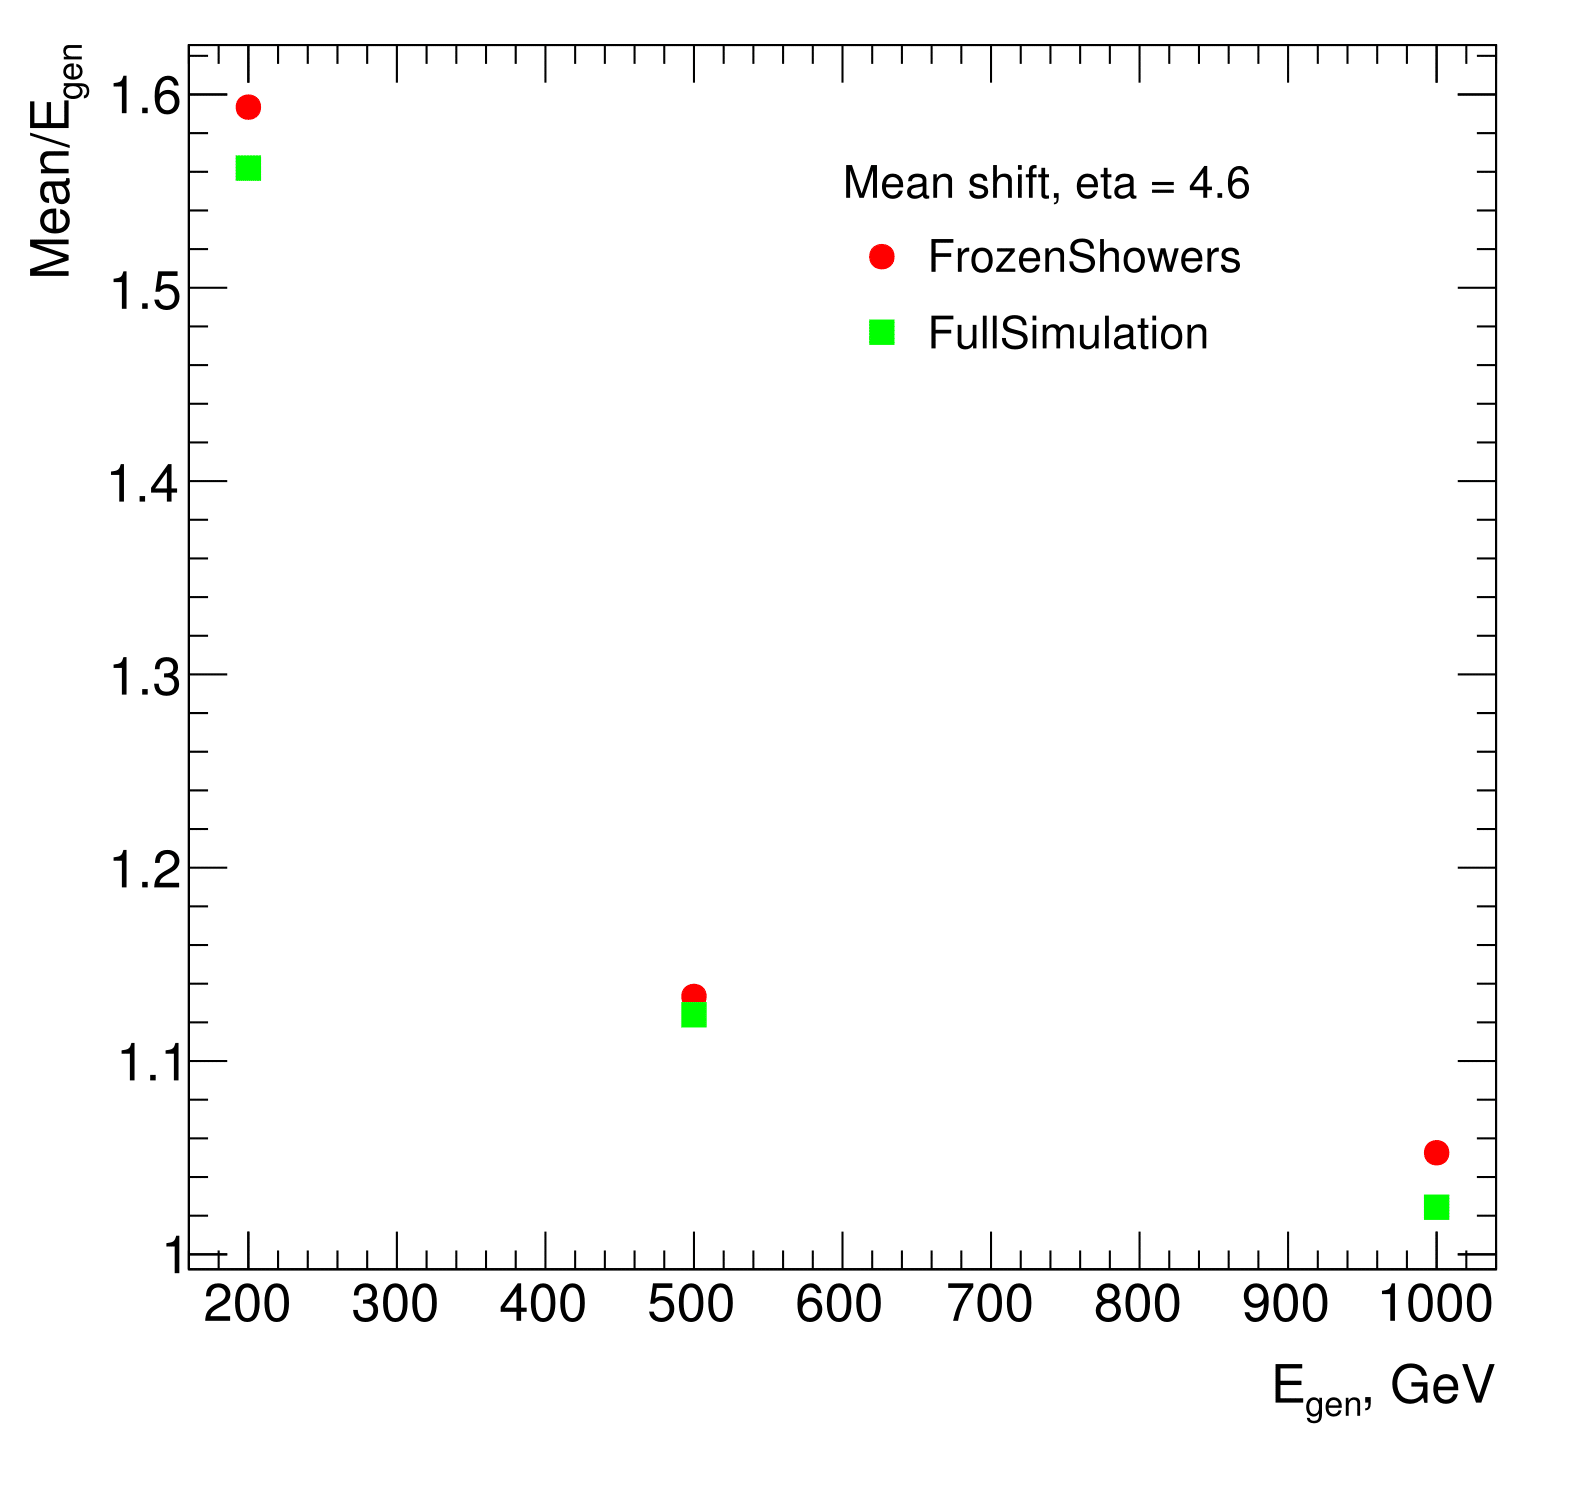
\includegraphics[width=1.\linewidth]{MC/Mean/Mean-01.png}  }
\end{minipage}
\caption{Shift of the reconstructed energy to the truth energy of electrons for full simulation, new FS libraries with ML binning and full simulation for different $\eta$ bins }
\label{fig:Mean}
\end{figure}

\subsection{Plans for the future}\label{sec:FSImpr}

The validation have showed a good agrement between full simulation and fast simulation for most of the bins, however, because not all of the bins are performing equally well, the additional modifications of the algorithm are needed. The following modifications have been investigated and planned to be performed in the nearest future:
\begin{itemize}
\item Procedure with $\eta$ dependent bin size. Currently all of the bins have the same size and position of the liquid argon bin. However, because of the outlying bins, the procedure should be modified and determine the bin position separately for each bin.
\item Use of the closer to real case for training sample. The problem of electron resolution could be also caused by too simlified models, used to train on. It is planned to repeat the procedure for training sample with distributions, closer to the nominal ones.
\item Adding the direction of the shower binned variable. Since there is a complicated dependency between position of the electron and its direction (especially in small energy region), the additional binning could solve the remaining problems with electron energy resolution.
\end{itemize}

\section{Validation of the new libraries}\label{sec:FSValidation}

The good fast simulation method should work equally good on all types of reconstructed objects, this is why for each new frozen showers libraries production an new iteration of mass validation is performed. The validation is done separately for each object by the different groups by comparing the distibutions obtained from full and fast simulation

Frozen showers have been validated on following objects and showed a good agreement:
\begin{itemize}
\item Z bosons from $Z \to ee$ sample with one central and one forward electrons(Fig. \ref{fig:OtherVal} a). The resolution of Z-mass peak is dominated by the resolution of the central electron, so Z boson is mostly sensitive just to the mean energy of the forward electrons. There is visible shift in the mass distribution between data and Monte-Carlo, that however, is within tolerable region.
\item Jets form two jet events. The validation have showed a good agreement for all of the variables. The distribution of the jet response (Fig. \ref{fig:OtherVal} b) showed, that Frozen Showers method does not change the jet scale.
\item Topo clusters from $t\bar{t}$ events. 
\item Forward electrons. The forward electrons validation have showed, that usage of the frozen showers is not changing the $\eta$ and $E_{T}$ distributions of the forward electrons. Studies of forward electrons resolution have been performed separately and will be discussed in the previous section.
\end{itemize}
The total agreement between full and fast simulation for different objects makes a Frozen Showers method applicable for a MC production in 2016.

\begin{figure}[!tbp]
\begin{minipage}[h]{0.49\linewidth}
\center{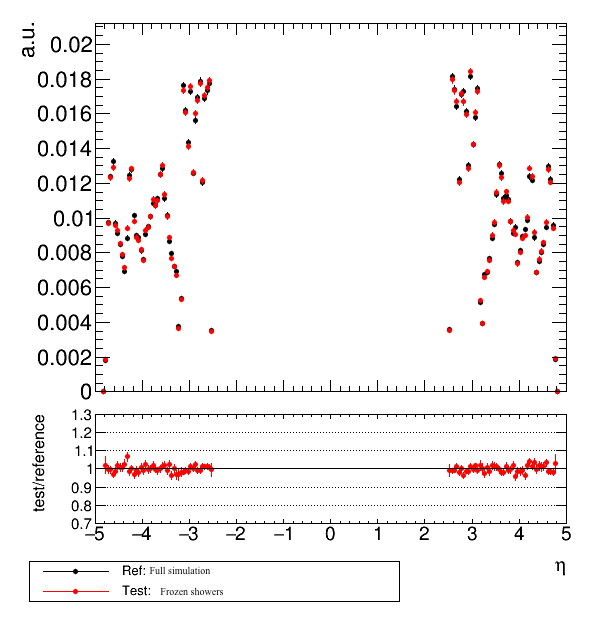
\includegraphics[width=1.\linewidth]{MC/Electron_Frwd_All_KinPlots_eta.png} \\ a)}
\end{minipage}
\hfill
\begin{minipage}[h]{0.49\linewidth}
\center{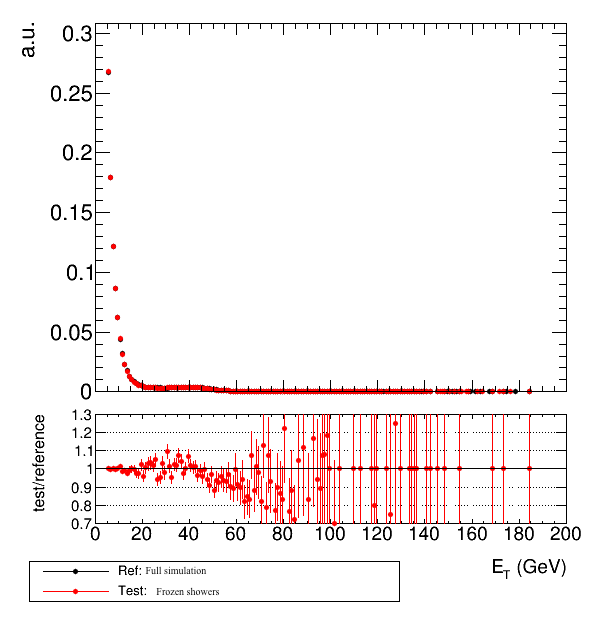
\includegraphics[width=1.\linewidth]{MC/Electron_Frwd_All_KinPlots_et.png} \\ b)}
\end{minipage}
\caption{Results of validation of the frozen showers library on forward electrons. Comparison between full simulation and fast simulation using frozen showers in forward electron events  for a) pseudorapditity and b) electron transverse energy  distributions. Modified from \cite{ElecForwardVal}. }
\label{fig:OtherValFwd}
\end{figure}

\begin{figure}[!tbp]
\begin{minipage}[h]{0.49\linewidth}
\center{\includegraphics[width=1.\linewidth]{MC/Zee_FWDZee_ZMassFWDTight.png} \\ a)}
\end{minipage}
\hfill
\begin{minipage}[h]{0.49\linewidth}
\center{\includegraphics[width=1.\linewidth]{MC/erhResponseVsEta.png} \\ b)}
\end{minipage}
\caption{ Results of validation of the frozen showers library on jets and $Z \to ee$ sample. Comparison between full simulation and fast simulation using frozen showers for and a) mass of the dilepton pair in $Z \to ee$ events (modified from \cite{ZeeVal}) b) jets responce vs  pseudorapditity  distribution (modified from \cite{JetsVal}) . }
\label{fig:OtherVal}
\end{figure}
